% Εκτύπωση σε χαρτί A4, μία σελίδα ανά φύλλο, με ξεχωριστή σελίδα για τον τίτλο,σε γραμματοσειρά 11pt και format βιβλίου.
\documentclass[a4paper,oneside,titlepage,11pt]{book}

% Πακέτα
\usepackage{fontspec}
\usepackage{xltxtra}
\usepackage{polyglossia}
\usepackage{xcolor,graphicx}
\usepackage{amsmath}
\usepackage{algorithm}
\usepackage{algorithmic}
\usepackage{caption}
\usepackage{cite}
\usepackage{setspace}
\usepackage[hmargin=3cm,vmargin=2.5cm]{geometry}
\usepackage{wrapfig}
\usepackage{mdwlist}
\usepackage{url}
\usepackage[labelfont={small,bf}, textfont={small}]{caption}
\usepackage{fancyvrb}
\usepackage{colortbl}

% Κενό μεταξύ γραμμών
\setstretch{1.2}

% Ορισμός γλωσσών για ορθογραφικό έλεγχο και hyphenation
\setmainlanguage[variant=mono,numerals=arabic]{greek}
\setotherlanguage{english}

% Γραμματοσειρές
\setmainfont{DejaVu Serif}
\setsansfont{DejaVu Sans}
\setmonofont{DejaVu Sans Mono}
%\newfontfamily\greekfont[Mapping=tex-text]{DejaVu Serif}
%\newfontfamily\greekfonttt[Mapping=tex-text]{DejaVu Sans}

% Μέγεθος Γραμματοσειρών για μαθηματικές παραστάσεις
\DeclareMathSizes{12}{14}{12}{12}

%\widowpenalty=2000
%\clubpenalty=2000

%Σελίδα Τίτλου
\begin{document}

\begin{titlepage}

\begin{wrapfigure}{l}{0.15\textwidth}
\vspace*{-11pt}
\includegraphics[width=0.15\textwidth]{./graphics/uoplogo.png}  
\end{wrapfigure}

\noindent Πανεπιστήμιο Πελοποννήσου\\
Σχολή Θετικών Επιστημών και Τεχνολογίας\\
Τμήμα Επιστήμης και Τεχνολογίας Υπολογιστών\\[3cm]

\vspace*{-10pt}

\begin{center}

{\LARGE {\noindent Πτυχιακή Εργασία}\\[2.5cm]

{\bf Υλοποίηση και Σύγκριση Αλγορίθμων Τομής Ευθείας-Τετραέδρου σε GPU\\[4cm]

Απόστολος-Ιάσων Κολιός}}\\[5cm]

\begin{Large}Επιβλέπων: {\bf Νίκος Πλατής}\end{Large}\\[3cm]

Τρίπολη, Μάρτιος 2012\\

\vfill
\end{center}
\end{titlepage}


%Περιλήψεις και κατάλογος σχημάτων
\frontmatter
\chapter*{Περίληψη}
\addcontentsline{toc}{chapter}{Περίληψη}
\pagestyle{plain}

\noindent Ο έλεγχος τομής ευθείας-τετραέδρου ανήκει σε μια κατηγορία προβλημάτων κεφαλαιώδους σημασίας για ένα μεγάλο αριθμό εφαρμογών στο πεδίο  των τριδιάστατων γραφικών. Παράλληλα, η πρόσφατη τάση προς την χρήση των μονάδων επεξεργασίας γραφικών (GPU) ως επεξεργαστών γενικού σκοπού έχει αποφέρει σημαντική αύξηση επιδόσεων σε ένα μεγάλο εύρος υπολογιστικά εντατικών εφαρμογών. Αντικείμενο της εργασίας αυτής είναι η μελέτη της εφαρμοσιμότητας των σύγχρονων τεχνικών προγραμματισμού GPU στους διαθέσιμους αλγορίθμους τομής ευθείας-τετραέδρου καθώς και η σύγκριση των επιδόσεων της προσέγγισης αυτής με τις παραδοσιακές υλοποιήσεις. Στα πλαίσια της εργασίας αυτής αναπτύχθηκε μια υλοποίηση των ταχύτερων αλγορίθμων τομής ευθείας-τετραέδρου σε μορφή κατάλληλη για εκτέλεση σε GPU.

Η παρούσα εργασία περιέχει τον τυπικό ορισμό του προβλήματος, την παρουσίαση των αλγορίθμων που χρησιμοποιούνται, την περιγραφή της υλοποίησης και τα συγκριτικά στοιχεία των επιδόσεων. Επίσης παρέχεται μια επισκόπηση των αρχιτεκτονικών των GPU και των τεχνικών προγραμματισμού τους.

\subsubsection*{Λέξεις-Κλειδιά}

\noindent Επεξεργασία σε GPU, Υπολογιστική Γεωμετρία, Έλεγχος τομής, Μαζική Παραλληλία, OpenCL, Ευθεία, Τετράεδρο, Παραλληλία SIMD 

\chapter*{Abstract}
\addcontentsline{toc}{chapter}{Summary}
\begin{english}
\noindent Ray-Tetrahedron intersection testing belongs to a class of computational problems that is fundamental to a wide range of applications in the field of 3D computer graphics. Additionally, the recent trend towards using Graphical Processing Units (GPUs) for general purpose computing has resulted in a significant performance increase in a wide number of computationally intensive applications. This project aims to determine the applicability of current GPU programming techniques to available ray-tetrahedron intersection algorithms and to compare the performance characteristics of this approach to traditional implementations. For the purposes of this project a GPU-targeted implementation of the fastest ray-tetrahedron intersection algorithms available has been developed. 

This report contains a formal definition of the ray-tetrahedron instersection problem, a presentation of the algorithms used, a description of the resulting implementation and data concerning its performance. Also provided is an overview of current GPU architectures and programming techniques.
\end{english} 

\subsubsection*{Keywords}

\noindent \begin{english}GPU Computing , Computational Geometry, Intersection Testing, Massive Parallelism, OpenCL, Ray, Tetrahedron, SIMD Parallelism\end{english} 


\renewcommand{\contentsname}{Περιεχόμενα}
\addcontentsline{toc}{chapter}{Περιεχόμενα}
\tableofcontents 
\cleardoublepage

\addcontentsline{toc}{chapter}{Κατάλογος Σχημάτων}
\listoffigures

%Κυρίως Κείμενο
\mainmatter
\chapter{Εισαγωγή}

\noindent Τα προβλήματα εντοπισμού τομής \begin{english}(intersection detection)\end{english} μεταξύ γεωμετρικών σχημάτων (στο επίπεδο) ή στερεών (στον χώρο) είναι μια ευρεία κατηγορία υπολογιστικών προβλημάτων με μεγάλο πλήθος εφαρμογών. Γενικά ορισμένο, ένα πρόβλημα εντοπισμού τομής μεταξύ δύο γεωμετρικών αντικειμένων περιγράφεται ως εξής:

\emph{«Με δεδομένα τα γεωμετρικά χαρακτηριστικά δύο αντικειμένων και των συντεταγμένων που ορίζουν την θέση τους, να βρεθεί
αν τα αντικείμενα τέμνονται. Αν τέμνονται, να προσδιοριστούν τα γεωμετρικά χαρακτηριστικά της τομής.»}

Η ύπαρξη αλγοριθμικών λύσεων υψηλής απόδοσης για τα προβλήματα εντοπισμού τομής είναι θεμελιώδους σημασίας για έναν μεγάλο αριθμό εφαρμογών 
σε έναν μεγάλο αριθμό διαφορετικών πεδίων. Παραδείγματα πεδίων στα οποία χρησιμοποιούνται οι λύσεις αυτές είναι, μεταξύ άλλων, τα γραφικά υπολογιστών (και ιδιαίτερα το animation), τα προγράμματα σχεδιασμού υποβοηθούμενου από υπολογιστή (CAD), τα συστήματα πλοήγησης, τα γεωγραφικά πληροφοριακά συστήματα (GIS) καθώς και ένα ευρύ φάσμα επιστημονικών
και μηχανικών εξομοιωτών.

Η εργασία αυτή θα επικεντρωθεί συγκεκριμένα στο πρόβλημα τομής ευθείας-τετραέδρου. Το συγκεκριμένο  πρόβλημα έχει ιδιαίτερη σημασία καθώς τα τελευταία χρόνια η χρήση τετραεδρικών πλεγμάτων (tetrahedral meshes) έχει εφαρμοστεί με επιτυχία για την αναπαράσταση περίπλοκων τριδιάστατων όγκων σε ένα μεγάλο εύρος εφαρμογών.      

Για το πρόβλημα τομής ευθείας-τετραέδρου έχουν προταθεί διάφοροι αλγόριθμοι με διαφορετικά επίπεδα απόδοσης. Στα πλαίσια της εργασίας αυτής χρησιμοποιείται ο αλγόριθμος που παρουσιάζεται στην δημοσίευση \cite{PlatisTheoharis03}, καθώς και μια τροποποίησή του που προτάθηκε από τον C. Ericson \cite{ericson2005real}\cite{ericson2007blog}.

Σκοπός της εργασίας αυτής είναι η ανάπτυξη μίας εναλλακτικής υλοποίησης των αλγορίθμων αυτών η οποία προορίζεται για εκτέλεση από μονάδες επεξεργασίας γραφικών (GPU). Η χρήση των GPU για την ταχεία εκτέλεση υπολογισμών γενικού σκοπού (όχι, δηλαδή, υπολογισμών που αφορούν άμεσα τον σχηματισμό εικόνας) γνωρίζει ραγδαία αύξηση τα τελευταία χρόνια. Η αρχιτεκτονική των σύγχρονων GPU, η οποία βασίζεται στο μοντέλο παραλληλίας SIMD (Single Instruction Multiple Data), επιτρέπει μια σημαντικότατη αύξηση επιδόσεων σε ορισμένες εφαρμογές σε σύγκριση τις επιδόσεις τους αν εκτελούνταν στην CPU. Όπως θα γίνει εμφανές στην συνέχεια, οι αλγόριθμοι τομής ευθείας-τετραέδρου που αναφέρθηκαν μπορούν να προσαρμοστούν σε τέτοια μορφή ώστε να εκμεταλλευτούν τα πλεονεκτήματα της αρχιτεκτονικής των GPU και να επιτύχουν αυξημένες επιδόσεις.   

Το κείμενο της εργασίας διαρθρώνεται ως εξής:
Το κεφάλαιο 2 περιέχει τον τυπικό ορισμό του προβλήματος τομής ευθείας-τετραέδρου και την παρουσίαση των αλγορίθμων που χρησιμοποιούνται, καθώς και των βελτιστοποιήσεων που εφαρμόζονται στους αλγορίθμους αυτούς.
Στο κεφάλαιο 3 παρουσιάζεται μια επισκόπηση των μεθόδων προγραμματισμού εφαρμογών προορισμένων προς εκτέλεση σε GPU. Αναλύεται επιγραμματικά η αρχιτεκτονική των σύγχρονων GPU, παρουσιάζονται τα σύγχρονα περιβάλλοντα προγραμματισμού και η ιστορία τους και εξηγείται ο τρόπος προσαρμογής του προβλήματος τομής ευθείας-τετραέδρου στην επίλυση σε GPU. 
Στο κεφάλαιο 4 αναλύεται ο τρόπος υλοποίησης του λογισμικού της εργασίας. Παρουσιάζεται αρχικά η ακολουθιακή (εκτελούμενη σε CPU) εκδοχή του προγράμματος και ο προϋπάρχων κώδικας στον οποίο βασίστηκε. Στην συνέχεια αναφέρεται σε γενικές γραμμές ο σχεδιασμός και η δομή της εκδοχής που προορίζεται προς εκτέλεση σε GPU. Επίσης δίνονται οδηγίες χρήσης των εκτελέσιμων της εργασίας.
Στο κεφάλαιο 5 περιγράφεται η μεθοδολογία μέτρησης της απόδοσης των διάφορων μορφών του λογισμικού της εργασίας και παρατίθεται η ερμηνεία των αποτελεσμάτων που προέκυψαν με επιλεγμένα παραδείγματα.
Τέλος, το παράρτημα Α περιέχει το σύνολο των αποτελεσμάτων που προέκυψαν απο τις μετρήσεις απόδοσης. 


\chapter{Τομή ευθείας-τετραέδρου}
\label{chapter:algs}
\section{Σημειολογία}
\subsection{Δεδομένα}
\label{chapter:alginput}
\noindent Στους αλγόριθμους που θα παρουσιαστούν στο παρόν κείμενο τα γεωμετρικά αντικείμενα (η ευθεία και το τετράεδρο) τα οποία ελέγχονται για την ύπαρξη τομής αναπαριστώνται ως εξής:

\emph{Ευθεία:} Η ευθεία στο συγκεκριμένο πρόβλημα είναι μια γραμμή άπειρου μήκους με συγκεκριμένη διεύθυνση και φορά. Η φορά της ευθείας επηρεάζει τα αποτελέσματα του αλγόριθμου, όπως θα προσδιοριστεί παρακάτω. Η ευθεία αναπαρίσταται από ένα σημείο $P$ επί αυτής και το διάνυσμα διεύθυνσής της, $L$. Στον κώδικα της υλοποίησης τα $P$ και $L$ είναι αντικείμενα που αντιπροσωπεύουν τριδιάστατα διανύσματα.  

\emph{Τετράεδρο:} Το τετράεδρο αναπαρίσταται από τις συντεταγμένες των τεσσάρων κορυφών του: $V_0,V_1,V_2,V_3$. Οι θέσεις των τεσσάρων κορυφών αντιπροσωπεύονται στον κώδικα της υλοποίησης από τριδιάστατα διανύσματα, παρομοίως με τα $P$ και $L$. Οι τέσσερις έδρες του τετραέδρου, $F_0,F_1,F_2,F_3,$ αριθμούνται με τον αριθμό της απέναντί τους κορυφής, ως εξής:

\begin{eqnarray*}
F_3 (V_0,V_1,V_2)\\	
F_2 (V_1,V_0,V_3)\\	
F_1 (V_2,V_3,V_0)\\		
F_0 (V_3,V_2,V_1)
\end{eqnarray*}
Στην περιγραφή του αλγόριθμου οι κορυφές της κάθε έδρας ονομάζονται ως εξής:\\
\begin{equation*}
 V^i_n
\end{equation*}
Όπου $i$ ο αριθμός της έδρας στην οποία ανήκει η κορυφή και $n$ ο αριθμός της κορυφής σε αυτή την έδρα, με την σειρά με την οποία παρατέθηκαν στην λίστα των εδρών. Για παράδειγμα, η κορυφή $V^3_0$  είναι η πρώτη  κορυφή της $F_3$, η $V_0$. Παρομοίως, οι ακμές της κάθε έδρας ονομάζονται ως εξής:

\begin{equation*}
e^i_k
\end{equation*}
Όπου $i$ ο αριθμός της έδρας στην οποία ανήκει η ακμή και $k$ ο αριθμός της απέναντί της κορυφής. Με αυτό τον τρόπο οι ακμές κατανέμονται ως εξής:

\begin{eqnarray*}
e^i_0 ({V^i_1 V^i_2})\\
e^i_1 ({V^i_2 V^i_0})\\	
e^i_2 ({V^i_0 V^i_1})		
\end{eqnarray*}
Για παράδειγμα, η ακμή $e^3_1$ ξεκινά από την κορυφή $V^3_2$  και καταλήγει στην $V^3_0$.\\

Οι αλγόριθμοι που θα παρουσιαστούν λειτουργούν με την παραδοχή ότι το τετράεδρο είναι προσανατολισμένο με τέτοιο τρόπο έτσι ώστε το κανονικό διάνυσμα κάθε έδρας $F_i$ να έχει τέτοια φορά  ώστε να απομακρύνεται από την αντίστοιχη κορυφή $V_i$. Ο προσανατολισμός του τετραέδρου είναι σημαντικός καθώς χρησιμοποιείται σε συσχετισμό με την φορά της ευθείας για να προσδιορίσει αν ένα σημείο τομής με την ευθεία είναι σημείο εισόδου ή εξόδου. Η διάκριση μεταξύ των σημείων εισόδου και εξόδου αναλύεται περαιτέρω στην ενότητα \ref{chapter:algs_pluck}.

\subsection{Ζητούμενα}
\label{chapter:algoutput}
\noindent Για κάθε ζεύγος ευθείας-τετραέδρου μπορεί να υπάρχει ή να μην υπάρχει τομή. Αν υπάρχει τομή, υπάρχουν τρεις περιπτώσεις, όπως φαίνονται στο σχήμα \ref{fig1}:

\begin{enumerate}
\item Η ευθεία τέμνει το τετράεδρο, άρα υπάρχουν δύο διακριτά σημεία $P_{enter}$ και $P_{leave}$ στα οποία η ευθεία εισέρχεται σε και εξέρχεται από το τετράεδρο αντίστοιχα.  

\item Η ευθεία τέμνει κάποια ακμή του τετραέδρου, άρα τα σημεία $P_{enter}$ και $P_{leave}$ ταυτίζονται.

\item Η ευθεία εφάπτεται σε κάποια έδρα του τετραέδρου, άρα υπάρχουν άπειρα σημεία τομής. Το σημείο στο οποίο η ευθεία εισέρχεται στην έδρα λογίζεται ως  $P_{enter}$ και αυτό από το οποίο εξέρχεται ως $P_{leave}$. 
\end{enumerate}
\pagebreak

\begin{figure}[t]
\center{ 
\includegraphics[scale=0.25]{graphics/raytetrarel0.png}
\includegraphics[scale=0.25]{graphics/raytetrarel1.png}
\includegraphics[scale=0.25]{graphics/raytetrarel2.png}}

\caption{Παραδείγματα των τριών περιπτώσεων τομής ευθείας-τετραέδρου.}
\label{fig1}
\end{figure}

Για κάθε τεμνόμενο ζεύγος ευθείας-τετραέδρου ο αλγόριθμος απαιτείται να υπολογίζει:

\begin{enumerate}
\item Τις καρτεσιανές συντεταγμένες των σημείων εισόδου και εξόδου, $P_{enter}$ και $P_{leave}$.  

\item Τις βαρυκεντρικές συντεταγμένες των σημείων εισόδου και εξόδου σε σχέση με τις έδρες ($F_{enter}$,$F_{leave}$) στις οποίες βρίσκονται. Συμβολίζονται ως $u^{enter}_1$,$u^{enter}_2$ και $u^{leave}_1$,$u^{leave}_2$. Για τις συντεταγμένες αυτές ισχύει ότι:

\begin{equation*}
P_k = (1 - u^k_1 - u^k_2)V^k_0 + u^k_1 V^k_1 + u^k_2 V^k_2
\end{equation*}
όπου $k= \text{enter} \text{ ή } \text{leave}$.
	
\item Τις παραμετρικές αποστάσεις $t_{enter}$ και $t_{leave}$ από το σημείο P το οποίο χρησιμοποιούμε για την αναπαράσταση της ευθείας. Για τις αποστάσεις αυτές ισχύει η σχέση:

\begin{equation*}
P_k = P +t_k L
\end{equation*}
όπου $k= \text{enter} \text{ ή } \text{leave}$.
\end{enumerate}
\pagebreak
\section{Αλγόριθμοι}
\label{chapter:algs_general}
\noindent  Στα πλαίσια της εργασίας αυτής δημιουργήθηκαν υλοποιημένες εκδόσεις δύο διαφορετικών αλγορίθμων. Οι δύο αυτοί αλγόριθμοι έχουν την ίδια βασική δομή. Ελέγχεται η ύπαρξη τομής μεταξύ της ευθείας και κάθε έδρας του τετραέδρου ξεχωριστά. Έτσι, ο έλεγχος τομής ευθείας-τετραέδρου αναλύεται σε τέσσερις ελέγχους τομής μεταξύ ευθείας και τριγώνου. Η διαφορά μεταξύ των δύο αλγορίθμων είναι η μέθοδος ελέγχου τομής ευθείας-τριγώνου που χρησιμοποιούν. Ο πρώτος βασίζεται στον έλεγχο τομής ευθείας-τριγώνου με συντεταγμένες Plücker που παρουσιάζεται στο ~\cite{PlatisTheoharis03}. Ο δεύτερος βασίζεται στον έλεγχο με χρήση μεικτού γινομένου τριών διανυσμάτων που αναφέρεται στο ~\cite{ericson2005real}.

Στην συνέχεια της ενότητας αυτής παρουσιάζονται οι δύο αυτές μέθοδοι ελέγχου τομής ευθείας-τριγώνου, το κοινό αλγοριθμικό πλαίσιο μέσω του οποίου συντίθεται ο έλεγχος τομής ευθείας-τετραέδρου και οι βελτιστοποιήσεις που επιδέχεται το πλαίσιο αυτό. 

\subsection{Τομή ευθείας-τριγώνου με συντεταγμένες Plücker}
\label{chapter:algs_pluck}
\noindent  Το σύστημα συντεταγμένων Plücker, που εισήχθη από τον Julius Plücker τον 19ο αιώνα\cite{plücker1828analytisch}, παρέχει μια μέθοδο ανάθεσης ομογενών συντεταγμένων σε κατευθυνόμενες ευθείες στον τριδιάστατο χώρο\cite{EricksonPlucker}. Στο σύστημα αυτό κάθε τέτοια ευθεία βρίσκεται σε 1-προς-1 αντιστοιχία με ένα εξαδιάστατο  διάνυσμα. Δεδομένης μια ευθείας $r$ η οποία ορίζεται από ένα σημείο $P$ και ένα διάνυσμα διεύθυνσης $L$, οι συντεταγμένες Plücker αυτής δίδονται από το διάνυσμα:

\begin{equation}
 \pi_r = \{L : L \times P ) = \{U_r : V_r\}		
\label{eq:plucker} 
\end{equation}

Μία από τις ιδιότητες των συντεταγμένων Plücker είναι ιδιαίτερα σημαντική για τους σκοπούς της εργασίας αυτής. Δεδομένων δύο ευθειών $r$ και $s$, το πρόσημο του αντιμετατεθημένου εσωτερικού γινομένου (permuted inner product) της σχέσης:

\begin{equation}
\pi_r \odot \pi_s = U_r \cdot V_s + U_s \cdot V_r	
\label{eq:permuted} 
\end{equation}
υποδεικνύει τον σχετικό προσανατολισμό των δύο ευθειών στο χώρο. Η έννοια του σχετικού προσανατολισμού δύο ευθειών στο χώρο επεξηγείται στο σχήμα \ref{fig:2}. 
\begin{figure}[b!]
1.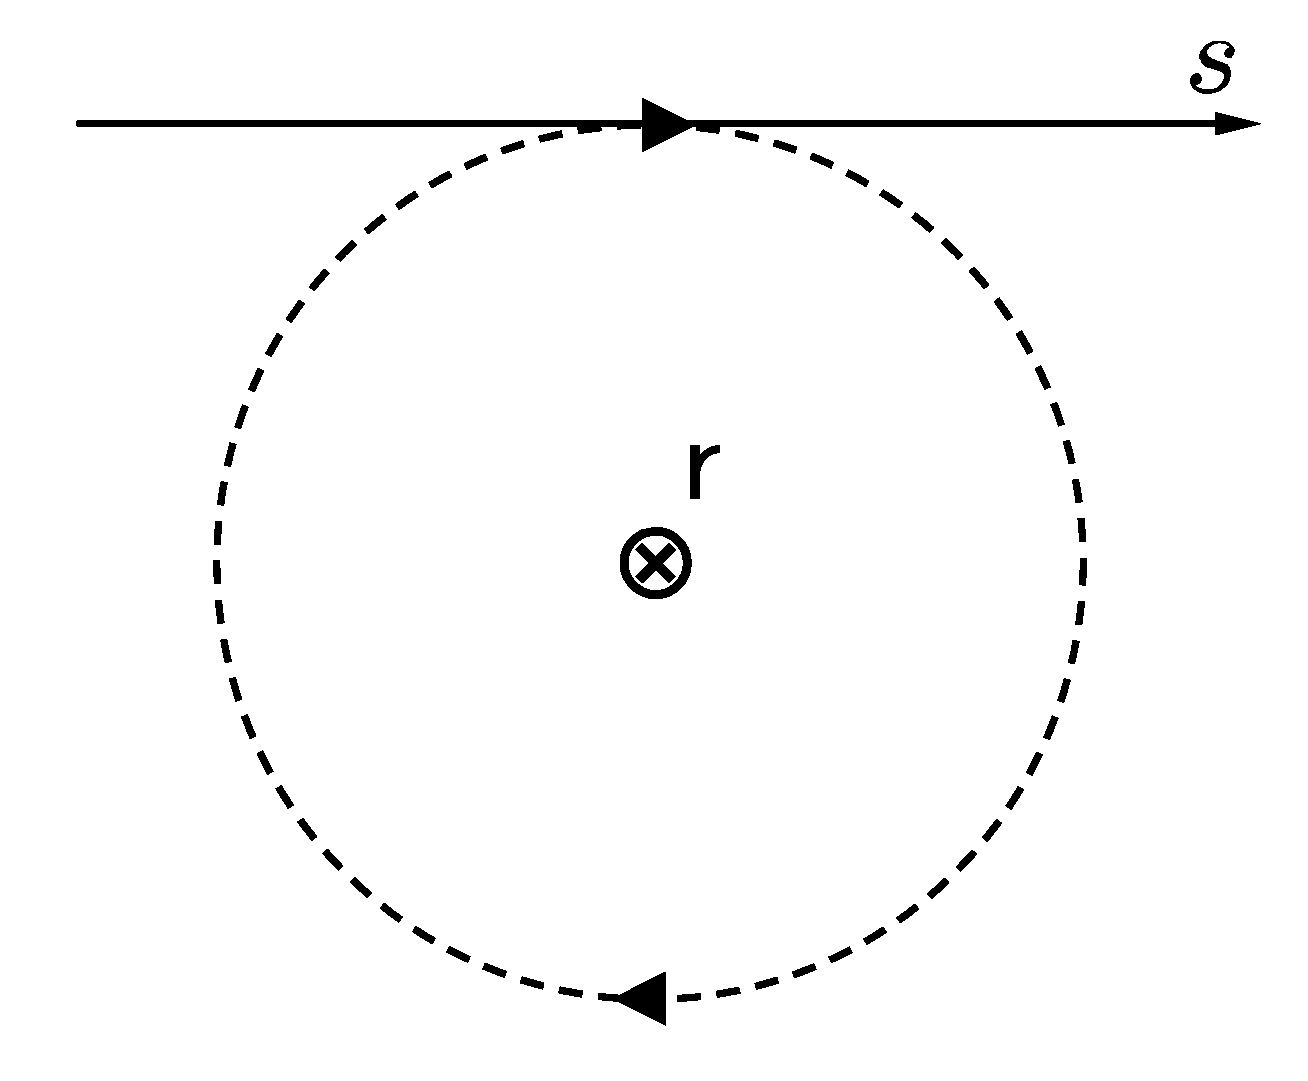
\includegraphics[scale=0.2]{graphics/orientations_cw.eps}
2.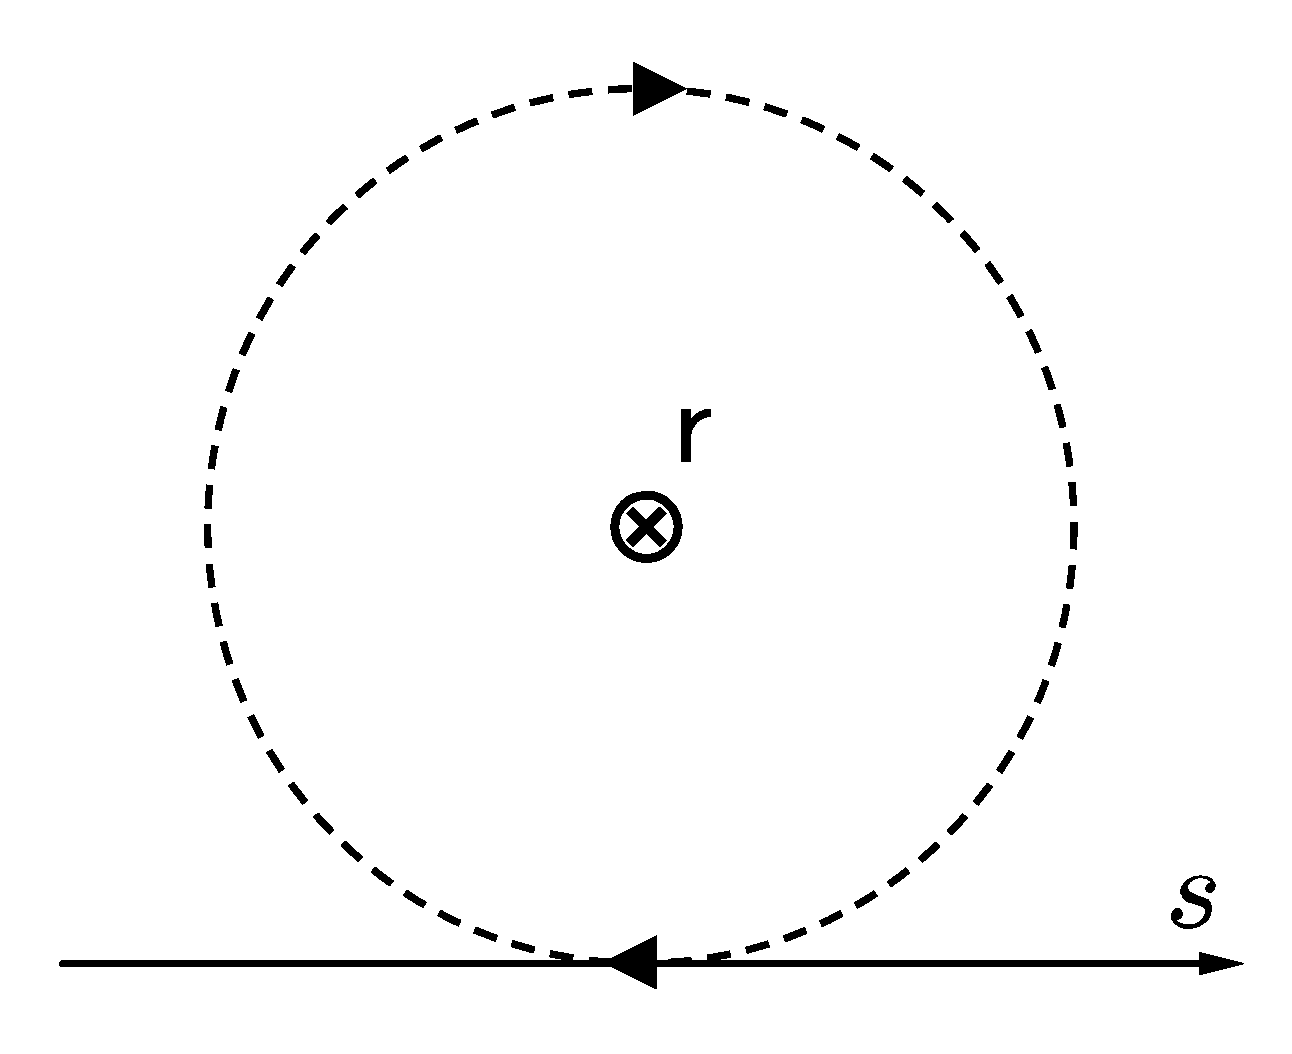
\includegraphics[scale=0.2]{graphics/orientations_ccw.eps}
3.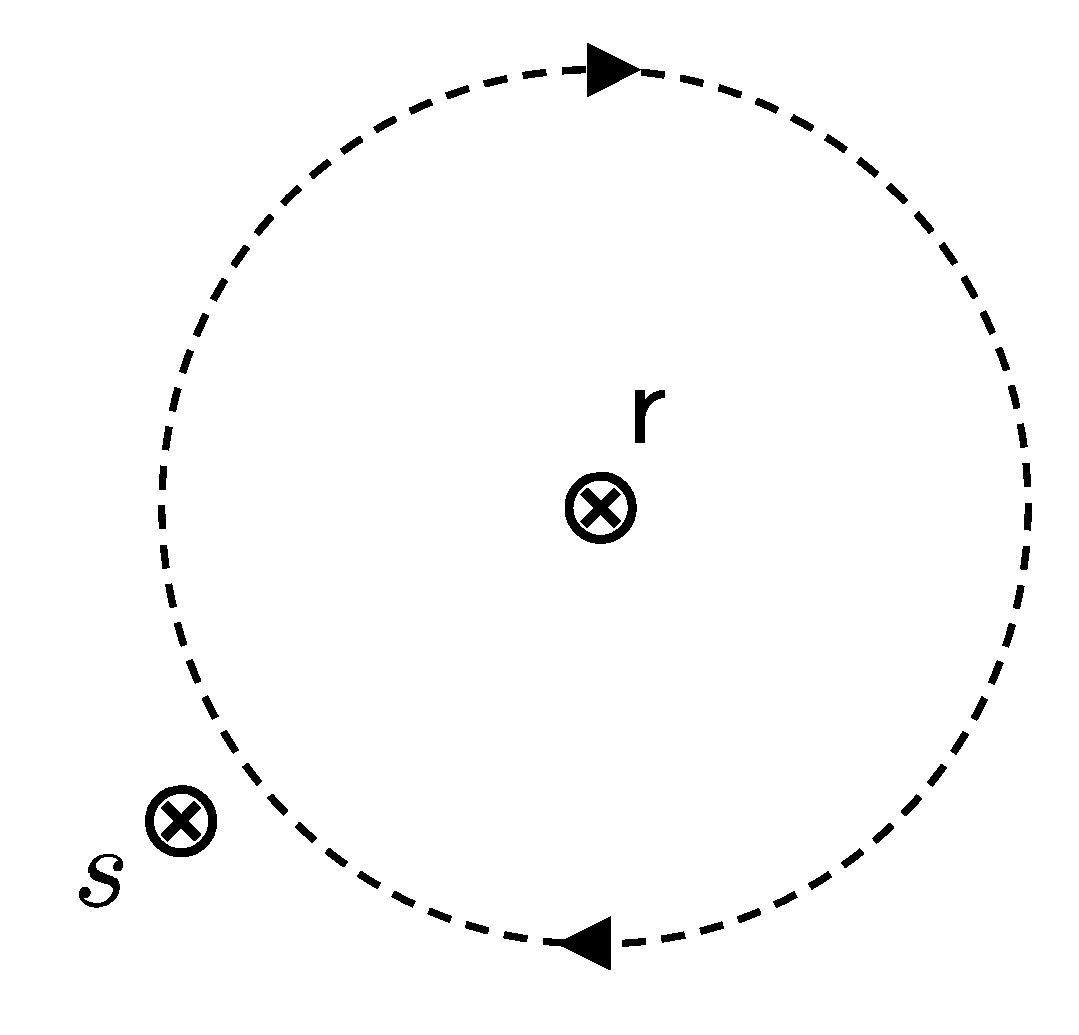
\includegraphics[scale=0.2]{graphics/orientations_parallel.eps}
\vspace*{20pt}\centering{4.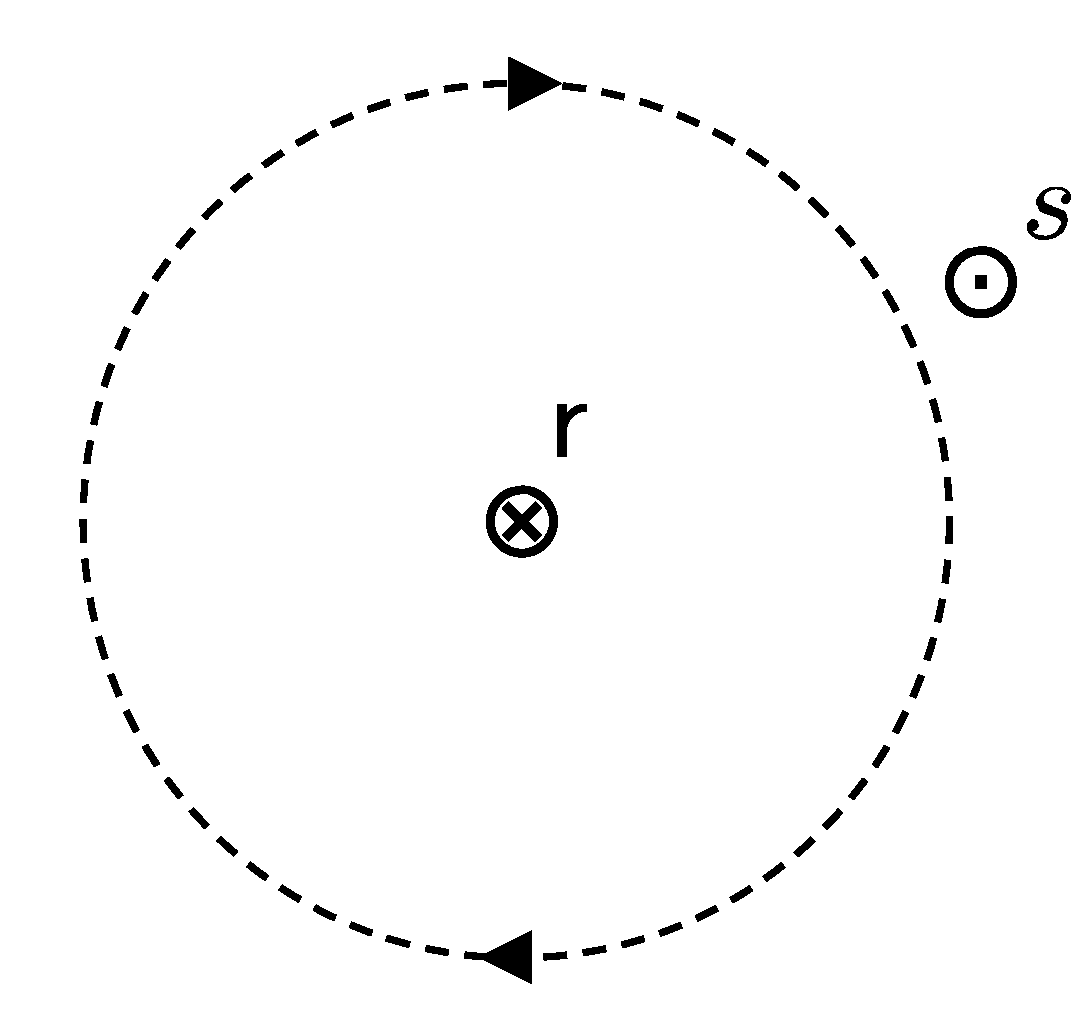
\includegraphics[scale=0.2]{graphics/orientations_antiparallel.eps}
5.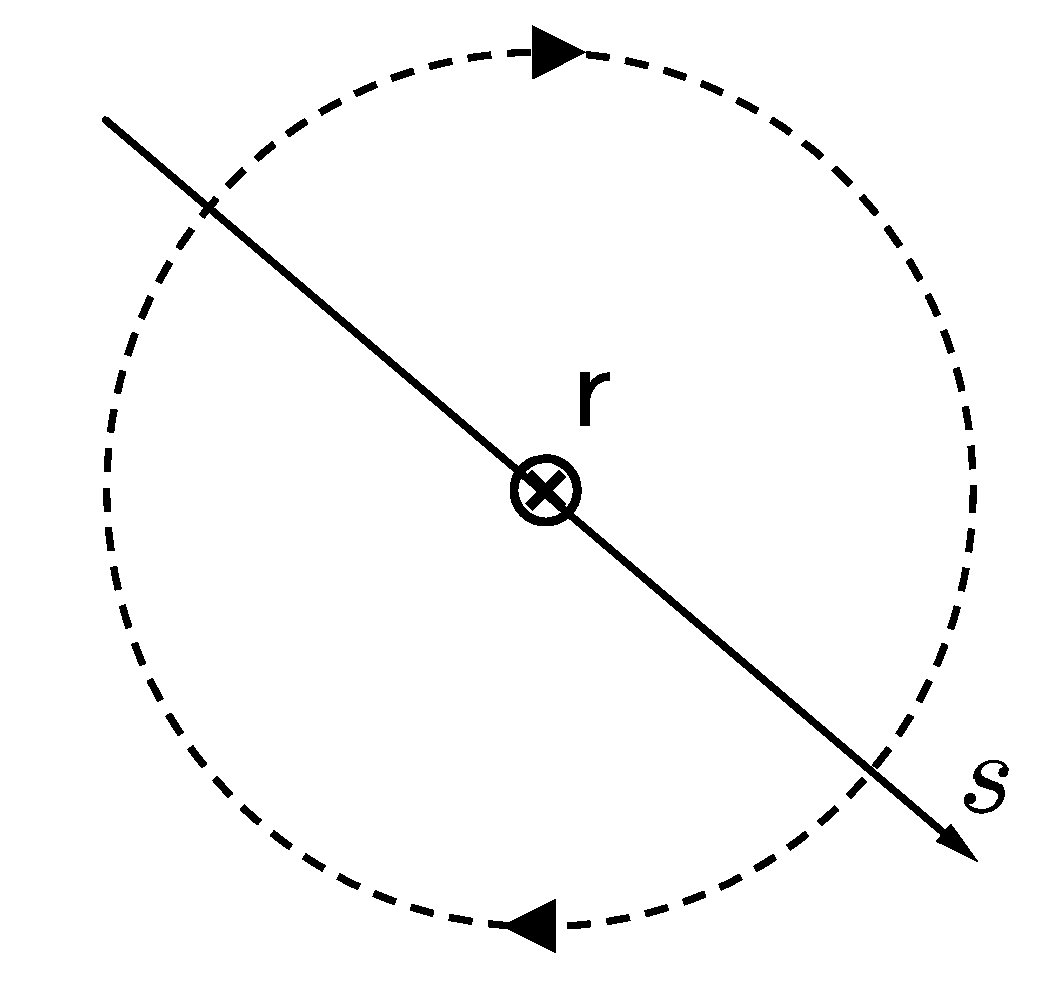
\includegraphics[scale=0.2]{graphics/orientations_intersect.eps}}
\captionsetup{singlelinecheck=off}
\caption[Σχετικός προσανατολισμός δύο κατευθυνόμενων ευθειών]{Σχετικός προσανατολισμός δύο κατευθυνόμενων ευθειών $r$ και  $s$ στον χώρο.  H ευθεία $r$ είναι κάθετη στο επίπεδο της σελίδας και την παρατηρούμε κοιτάζοντας κατά την κατεύθυνσή της. Οι περιπτώσεις είναι οι εξής:\begin{enumerate}\item H $s$ στρέφεται με φορά ρολογιού σε σχέση με την $r$.\item H $s$ στρέφεται  με φορά  αντίθετη του ρολογιού σε σχέση με την $r$.\item H $s$ είναι παράλληλη στην $r$.\item H $s$ είναι αντιπαράλληλη στην $r$.\item H $s$ τέμνει την $r$.\end{enumerate}}
\label{fig:2}
\end{figure} 

Το πρόσημο του αντιμετατεθημένου εσωτερικού γινομένου της σχέσης \eqref{eq:permuted} αντιστοιχεί στον σχετικό προσανατολισμό των $r$ και $s$ ως εξής: 

\begin{enumerate}

\item
$\pi_r \odot \pi_s > 0\iff$Η $s$ στρέφεται με φορά ρολογιού σε σχέση με την $r$.
\item
$\pi_r \odot \pi_s < 0\iff$Η $s$ στρέφεται με φορά αντίθετη του ρολογιού σε σχέση με την $r$.
\nolinebreak\item 
$\pi_r \odot \pi_s = 0\iff$Η $s$ τέμνει ή είναι παράλληλη στην $r$.\\
\label{linecrit}
\end{enumerate}

Με βάση την ιδιότητα αυτή μπορεί να αναπτυχθεί η εξής μέθοδος για τον έλεγχο τομής ευθείας-τριγώνου:\\

Έστω ευθεία $r$ και τρίγωνο $\Delta(V_0,V_1,V_2)$ με ακμές $e_0(V_1V_2)$, $e_1(V_2V_0)$, $e_2(V_0V_1)$. Ισχύει ότι η $r$ τέμνει το $\Delta$ \textbf{αν και μόνο αν} έχει τον ίδιο σχετικό προσανατολισμό και με τις τρεις ακμές $e_0,e_1,e_2$ ή αν τέμνει το πολύ δύο από αυτές. Άρα, ισχύουν τα ακόλουθα:

\begin{enumerate}
\item
Η $r$ τέμνει (εισερχόμενη) το $\Delta$ αν: \begin{equation*}\pi_r \odot \pi_{e_{i}} \geq 0\; \forall\; i\in \{0,1,2\}\; KAI \; \exists \,j : \pi_r \odot \pi_{e_{j}} \neq 0\end{equation*}
\item
Η $r$ τέμνει (εξερχόμενη) το $\Delta$ αν:\begin{equation*}\pi_r \odot \pi_{e_{i}} \leq 0\; \forall\; i\in \{0,1,2\}\;  KAI \; \exists \,j : \pi_r \odot \pi_{e_{j}} \neq 0 \end{equation*}
\item
Η $r$ είναι συνεπίπεδη με το $\Delta$ αν: \begin{equation}\pi_r \odot \pi_{e_{i}}= 0 \;\forall\; i\in \{0,1,2\}\; \label{eq:crit}  \end{equation}
\end{enumerate}

Στις περιπτώσεις 1 και 2 οι τιμές των αντιμετατεθημένων εσωτερικών γινομένων $\pi_r \odot \pi_{e_{i}}$ παρέχουν άμεσα τις βαρυκεντρικές συντεταγμένες του σημείου τομής $P_k$ ως προς τις κορυφές $V_{0,1,2}$, όπως αποδεικνύεται στο ~\cite{JonesIntersect}. Έστω:\\
\begin{equation}w^k_i=\pi_r \odot \pi_{e_{i}}
\label{eq:bary1} 
\end{equation}
H συνισταμένη $u^k_i$ των βαρυκεντρικών συντεταγμένων του σημείου τομής $P_k$ ως προς την κορυφή $V_i$ ισούται με:
\begin{equation}
u^k_i = \frac{w^k_i}{\displaystyle\sum_{i=0}^{3} w^k_i}  \qquad
\label{eq:bary2} 
\end{equation}
Οι καρτεσιανές συντεταγμένες του σημείου $P_k$ μπορούν να βρεθούν ως εξής:

\begin{equation}
P_k = u^k_0 V_0 + u^k_1 V_1 + u^k_2 V_2
\label{eq:cart} 
\end{equation}
Επιπλέον, η παραμετρική απόσταση από το σημείο $P$ επί της ευθείας μπορεί να υπολογιστεί λύνοντας ως προς $t_k$ την σχέση

\begin{equation}
P_k = P + t_k L
\label{eq:para} 
\end{equation}
για οποιαδήποτε μη-μηδενική συνισταμένη των συντεταγμένων του διανύσματος διεύθυνσης $L$.

\subsection{Τομή ευθείας-τριγώνου με μεικτό γινόμενο}
\label{chapter:stpalg}
\noindent  Η προσέγγιση αυτή βασίζεται σε μια εναλλακτική μέθοδο υπολογισμού του σχετικού προσανατολισμού δύο ευθειών που παρουσιάζεται στα ~\cite{ericson2005real} και ~\cite{ericson2007blog} από τον C. Ericson. Η μέθοδος αυτή απορρέει από την διαπίστωση ότι, στα πλαίσια της εύρεσης του σχετικού προσανατολισμού δύο κατευθυνόμενων ευθύγραμμων τμημάτων (και κατ' επέκταση ευθειών), το αντιμετατεθημένο εσωτερικό γινόμενο της σχέσης \eqref{eq:permuted} είναι μαθηματικώς ισοδύναμο με το μεικτό γινόμενο τριών διανυσμάτων τα οποία αντιπροσωπεύουν τα δύο ευθύγραμμα τμήματα.

Έστω δύο κατευθυνόμενα ευθύγραμμα τμήματα $AB$ και $CD$. Ορίζονται τα διανύσματα $\vec{p} = B -A$, $\vec{q} = C -A$, $\vec{r} = D -A$ όπως φαίνονται στο σχήμα ~\ref{fig3}.
\begin{figure}[t!]
\centering{\includegraphics[scale=0.6]{graphics/stp.png}}
\caption{Αντιστοιχία των διανυσμάτων p,q,r με τα ευθύγραμμα τμήματα AB και CD. }
\label{fig3}
\end{figure}
\begin{figure}[b!]
\centering{\includegraphics[scale=0.6]{graphics/stp_volume.png}}
\caption{Το παραλληλεπίπεδο που ορίζεται από τα διανύσματα p,q,r.}
\label{fig4}
\end{figure}
Η ποσότητα $\vec{p} \cdot (\vec{q} \times \vec{r})$ ονομάζεται  μεικτό γινόμενο των $\vec{p},\vec{q},\vec{r}$ και μπορεί να συμβολιστεί ως $[p q r]$. Το μεικτό γινόμενο έχει την ιδιότητα να είναι αμετάβλητο για οποιοδήποτε πιθανή κυκλική μετάθεση των στοιχείων του, δηλαδή ισχύει:

\begin{equation}
[p q r] = [r p q] = [q r p]
 \label{eq:circular}
\end{equation}

Οι μη κυκλικές μεταθέσεις προκύπτουν με απλή αλλαγή του προσήμου:

\begin{equation}
[p q r] = -[q p r]\;\;,\;\;[q p r] = -[r p q] \;\;\text{κ.ο.κ.}
\label{eq:noncircular}
\end{equation}

Το μεικτό γινόμενο $[p q r]$ μπορεί να χρησιμοποιηθεί για την εύρεση του σχετικού προσανατολισμού των $AB$ και $CD$ στον χώρο ακριβώς όπως το αντιμετατεθημένο εσωτερικό γινόμενο των συντεταγμένων Plücker της σχέσης \eqref{eq:permuted}. Απόδειξη της ισοδυναμίας των δύο μεθόδων υπάρχει στην δημοσίευση \cite{kensler:06:triangle}. Η ισοδυναμία αυτή προκύπτει από το γεγονός ότι τα δύο αυτά μεγέθη αντιστοιχούν στην ίδια γεωμετρική ποσότητα, τον προσημασμένο όγκο του παραλληλεπιπέδου ο οποίος ορίζεται από τα τρία αυτά διανύσματα (σχήμα \ref{fig4}). Ο όγκος αυτός είναι προσημασμένος καθώς εξαρτάται από τον σχετικό προσανατολισμό των $p$,$q$,$r$ και κατ' επέκταση των $AB$,$CD$.

Στην περίπτωση που εξετάζουμε ισχύει ότι:

\begin{enumerate}
\item
 Αν $[p q r] > 0\iff$Το $CD$ στρέφεται με φορά ρολογιού σε σχέση με το $AB$.
\item
Αν $[p q r] < 0\iff$Το $CD$ στρέφεται με φορά αντίθετη του ρολογιού σε σχέση με το $AB$.
\item
Αν $[p q r] = 0\iff$ Το $CD$ τέμνει ή είναι παράλληλο προς το $AB$.\\
\end{enumerate}
Ο έλεγχος τομής ευθείας-τριγώνου που παρουσιάστηκε στην προηγούμενη ενότητα μπορεί να πραγματοποιηθεί ισοδύναμα με την χρήση μεικτού γινομένου. Στην περίπτωση αυτή το ευθύγραμμο τμήμα $AB$ αντιστοιχεί σε αυτό που ορίζεται από τα σημεία $P$ και $L$ (με φορά από το $P$ προς το $L$) και το $CD$ στην εκάστοτε ακμή του τριγώνου (με την φορά της ακμής). Για παράδειγμα, στον έλεγχο σχετικού προσανατολισμού της ευθείας με την ακμή $e_0(V_1V_2)$  τα αντίστοιχα διανύσματα $p$,$q$,$r$ είναι τα εξής: $p=L$, $q=V_0-P$, $ r=V_1-P$. Αντίστοιχα προσαρμόζεται ο έλεγχος των υπόλοιπων ακμών.

\subsection{Βασικός αλγόριθμος τομής ευθείας-τετραέδρου}
\label{chapter:raytetraint}
\noindent  Με βάση τον έλεγχο τομής ευθείας-τριγώνου που αναφέρθηκε μπορεί να αναπτυχθεί εύκολα ένας βασικός αλγόριθμος τομής ευθείας-τετραέδρου. Ο αλγόριθμος ελέγχει κάθε έδρα του τετραέδρου με την σειρά με βάση τα κριτήρια της παράστασης \eqref{eq:crit}. Aν κάποια από τις έδρες διαπιστωθεί οτι είναι η έδρα εισόδου ($F_{enter}$) ή η έδρα εξόδου ($F_{leave}$) τότε ο αντίστοιχος έλεγχος δεν πραγματοποιείται για τις υπόλοιπες έδρες. 

Στην συνέχεια του κειμένου, όταν γίνεται αναφορά στην έδρα $F_i$ του τετραέδρου θα συμβολίζονται ως $\pi^i_j$ οι συντεταγμένες Plücker της ακμής $e^i_j$  και ως $\sigma^i_j$ το πρόσημο του αντιμετατεθημένου εσωτερικού γινομένου $\pi_r \odot \pi^i_j$ για την δεδομένη ευθεία $r$ ή του ισοδύναμου μεικτού γινομένου. Επίσης, ως ${e^i_j}_{(\alpha)}$ και ${e^i_j}_{(\beta)}$ συμβολίζονται η αρχική και τελική (σύμφωνα με την φορά) κορυφή της έδρας $e^i_j$. Ισχύει ότι:

\begin{equation}
\sigma^i_j =\text{sign}(\pi_r \odot \pi^i_j) = \text{sign}(\;[L({e^i_j}_{(\alpha)}-P)({e^i_j}_{(\beta)}-P)]\;)\\ 
\label{eq:sigmatostp} 
\end{equation}
\begin{equation}
\sigma^i_j =
\begin{cases}
 \;\; \;1,\;\text{αν}\,\pi_r \odot \pi^i_j>0\text{ ή, ισοδύναμα,} \;[L({e^i_j}_{(\alpha)}-P)({e^i_j}_{(\beta)}-P)]\;>0 \\
 \;\; \;0,\;\text{αν}\,\pi_r \odot \pi^i_j=0\text{ ή, ισοδύναμα,} \;[L({e^i_j}_{(\alpha)}-P)({e^i_j}_{(\beta)}-P)]\;=0 \\
 \; -1,\;\text{αν}\,\pi_r \odot \pi^i_j<0\text{ ή, ισοδύναμα,} \;[L ({e^i_j}_{(\alpha)}-P)({e^i_j}_{(\beta)}-P)]<0 \\
\end{cases}
\end{equation}

Ο αλγόριθμος εκφράζεται σε ψευδοκώδικα ως εξής:
\floatname{algorithm}{Αλγόριθμος}
\begin{algorithm}[H]
\caption{Ο βασικός αλγόριθμος Τομής Ευθείας-Τετραέδρου}
\label{segura0}
\begin{algorithmic}
\STATE $F_{enter} \gets nil$
\STATE $F_{leave} \gets nil$
\FOR{$ i = 3, 2, 1, 0$}
\STATE Υπολογισμός $\sigma^i_0$,$ \sigma^i_1$,$\sigma^i_2$
\IF{$ (( \sigma^i_0 \neq 0)$ \OR $( \sigma^i_1  \neq 0)$ \OR  $(\sigma^i_2  \neq 0))$}
\IF{ $((F_{enter} == nil)$ \AND $ \sigma^i_0 \geq 0)$ \AND $( \sigma^i_1 \geq 0)$ \AND $( \sigma^i_2 \geq 0))$}
\STATE$ F_{enter} \gets F_i$
\ELSIF {$((F_{leave} == nil)$ \AND $( \sigma^i_0 \leq 0)$ \AND  $(\sigma^i_1 \leq 0)$ \AND $(\sigma^i_2 \leq 0))$}
\STATE$ F_{leave} \gets F_i$
\ENDIF
\ENDIF
\ENDFOR
\end{algorithmic}
\end{algorithm}

Ο αλγόριθμος αυτός μπορεί επιπρόσθετα να χρησιμοποιηθεί  για τον υπολογισμό των βαρυκεντρικών συντεταγμένων χρησιμοποιώντας τις σχέσεις \eqref{eq:bary1} και \eqref{eq:bary2}. Ομοίως, οι σχέσεις \eqref{eq:cart}
και \eqref{eq:para} μπορούν να χρησιμοποιηθούν για τον υπολογισμό των καρτεσιανών συντεταγμένων του σημείου τομής και των παραμετρικών αποστάσεων από το $P$ αντίστοιχα. Επίσης μπορούν να εντοπιστούν εύκολα οι ειδικές περιπτώσεις στις οποίες η ευθεία εφάπτεται σε κάποια ακμή ή έδρα του τετραέδρου, καθώς στις περιπτώσεις αυτές ένα ή δύο από τα $\sigma^i_j$ για κάποια τιμή του $i$ ισούνται με 0.

Στην υλοποίηση η οποία έγινε στα πλαίσια της εργασίας, η βασική αυτή μορφή του αλγορίθμου ονομάζεται μορφή 0.  

\subsection{Βελτιστοποιήσεις}

\noindent Ο αλγόριθμος που παρουσιάστηκε στην ενότητα \ref{chapter:raytetraint} επιδέχεται πολλές βελτιστοποιήσεις. Οι βελτιστοποιήσεις αυτές προέρχονται από τρεις βασικές τροποποιήσεις του τρόπου λειτουργίας του αλγορίθμου:

\begin{itemize}
\item Την απαλοιφή των μη απαραίτητων ελέγχων.
\item Την επανάληψη χρήσης των ήδη υπολογισμένων ποσοτήτων για διαφορετικές έδρες του τετραέδρου.
\item Την αξιοποίηση των γεωμετρικών χαρακτηριστικών του προβλήματος.  
\end{itemize}

Οι βελτιστοποιήσεις που ακολουθούν βασίζονται στις πρώτες δύο τροποποιήσεις και προέρχονται από τις ενότητες 3.1 και 3.2 του \cite{PlatisTheoharis03}.

\begin{enumerate}
\item Ο αλγόριθμος μπορεί να τερματίσει άμεσα αν έχουν προσδιοριστεί τα $F_{enter}$ και $F_{leave}$ χωρίς να εξετάσει τις υπόλοιπες έδρες του τετραέδρου.
\item Μόνο τρεις από τις τέσσερις έδρες του τετραέδρου είναι απαραίτητο να ελεγχθούν. Αν και οι τρεις δεν τέμνονται από την ευθεία τότε είναι αδύνατον να τέμνεται η τέταρτη. Αν κάποια από τις τρεις τέμνεται τότε και η τέταρτη θα τέμνεται. Η τέταρτη έδρα θα είναι η $F_{enter}$ αν έχει ήδη βρεθεί η $F_{leave}$ ή η $F_{leave}$ αν έχει ήδη βρεθεί η $F_{enter}$. 
\item Κάθε ακμή του τετραέδρου ανήκει σε δύο διαφορετικές έδρες και διατρέχεται με αντίθετη φορά σε καθεμία από αυτές. Η τιμή του $\sigma$ χρειάζεται να υπολογιστεί μόνο μία φορά για κάθε ακμή. Το $\sigma$ της ακμής με τις ίδιες κορυφές και αντίθετη φορά προκύπτει με απλή αλλαγή του προσήμου του ήδη υπολογισμένου. Για παράδειγμα, η $e^3_2$ $(V_{0}V_{1})$ και η $e^2_2$ $(V_{1}V_{0})$ διαφέρουν μόνο κατά την φορά. Ισχύει ότι:
\begin{equation*}
\pi_r \odot \pi^3_2 = -(\pi_r \odot \pi^2_3)
\end{equation*}
\begin{equation*}
[L (V_1-P) (V_0-P)] = - [L (V_0-P) (V_1-P)]
\end{equation*}

Στην περίπτωση της χρήσης συντεταγμένων Plücker η ιδιότητα αυτή προκύπτει από τον ορισμό των συντεταγμένων Plücker και του αντιμετατεθημένου εσωτερικού γινομένου. Στην περίπτωση του μεικτού γινομένου προκύπτει από την σχέση \ref{eq:noncircular}.
\item Όταν έχει βρεθεί μία έδρα που τέμνεται από την ευθεία και απομένουν μόνο δύο έδρες προς έλεγχο είναι δυνατόν να προσδιοριστεί η άλλη τεμνόμενη έδρα πραγματοποιώντας μόνο ένα υποσύνολο των συγκρίσεων προσήμων που χρειάζονται στην γενική περίπτωση. Η επιλογή ανάμεσα στις δύο έδρες βασίζεται στο πρόσημο της κοινής τους ακμής. Για παράδειγμα, έστω ότι πρέπει να βρεθεί ποια από τις $F_1(V_2V_3V_0)$ και $F_0(V_3V_2V_1)$ είναι η $F_{leave}$. Αν $\pi_r \odot \pi_{V_2V_3} < 0$ τότε $F_{leave}$ είναι η $F_1$, αλλιώς είναι η $F_0$. Εξαίρεση αποτελεί η περίπτωση στην οποία όλα τα $\sigma^0_j$ είναι 0 οπότε ισχύει ότι $F_{leave}$ είναι η $F_1$. 
\item Στον βασικό αλγόριθμο ο έλεγχος κάθε έδρας του τετραέδρου περιλαμβάνει τον υπολογισμό και των τριών ποσοτήτων $\sigma^i_j$. Όμως, αν δύο από αυτές δεν έχουν το ίδιο πρόσημο τότε δεν είναι απαραίτητο να υπολογιστεί και να συγκριθεί η τρίτη. Η βελτιστοποίηση αυτή περιπλέκεται από το γεγονός ότι ένα ή δύο από τα $\sigma^i_j$ μπορεί να ισούνται με 0. Η βελτιστοποιημένη εκδοχή του έλεγχου για την έδρα $F_i$ είναι η εξής:

\floatname{algorithm}{Αλγόριθμος}
\begin{algorithm}[H]
\caption{Βελτιστοποίηση του ελέγχου έδρας}
\label{segura1inner}
\begin{algorithmic}
\STATE Υπολογισμός $\sigma^i_0$ και $\sigma^i_1$.
\STATE \{Έλεγχος ισότητας των $\sigma^i_0$ και $\sigma^i_1$ μεταξύ τους και με το 0. Αν διαφέρουν και είναι μη μηδενικά δεν υπάρχει τομή με αυτή την έδρα.\}
\IF{(($\sigma^i_0 == \sigma^i_1$ ) \OR ($\sigma^i_0 == 0$) \OR ($\sigma^i_1 == 0$))}

\STATE Υπολογισμός $\sigma^i_2$
\STATE \{Εύρεση του προσήμου $\sigma^i$ της έδρας. Το $\sigma^i$ είναι ίσο με το πρώτο από τα  $\sigma^i_0$ και $\sigma^i_1$ που είναι μη μηδενικό, ή το $\sigma^i_2$ αν και τα δύο είναι μηδενικά.\}

\STATE $\sigma^i =\gets \sigma^i_0$

\IF{($\sigma^i == 0$)}

\STATE $\sigma^i \gets \sigma^i_1$

\IF{($\sigma^i == 0$)}

\STATE $\sigma^i \gets \sigma^i_2$
\ENDIF
\ENDIF
\STATE \{Για να υπάρχει τομή πρέπει το $\sigma^i_2$ να έχει ίδιο πρόσημο με το $\sigma^i$, ή να είναι μηδενικό. Στην περίπτωση που το $\sigma^i$ είναι μηδενικό η ευθεία είναι συνεπίπεδη με την έδρα.\}

\IF{(($\sigma^i \neq 0$) \AND ($(\sigma^i_2 == \sigma^i $) \OR $(\sigma^i_2 == 0$)))}
\STATE \{Διάκριση μεταξύ έδρας εισόδου και εξόδου.\}
\IF {$(\sigma^i > 0$)}
\STATE $F_{enter} \gets F_i$
\ELSE
\STATE $F_{leave} \gets F_i$
\ENDIF
\ENDIF
\ENDIF
\end{algorithmic}
\end{algorithm}
   
\item Όταν βρεθεί μία έδρα η οποία τέμνεται από την ευθεία ο βελτιστοποιημένος έλεγχος που παρουσιάστηκε μπορεί να απλοποιηθεί περαιτέρω για τις έδρες που απομένουν. Οι ακμές της τεμνόμενης έδρας που είναι κοινές με τις υπόλοιπες έδρες έχουν γνωστό πρόσημο $\sigma$ (βλ. βελτιστοποίηση 3) και ο έλεγχος για τις υπόλοιπες ακμές απλοποιείται στο $\sigma^i_j \leq 0$ αν έχει βρεθεί η $F_{enter}$ ή $\sigma^i_j \geq 0$ αν έχει βρεθεί η $F_{leave}$.
\end{enumerate}

Στον κώδικα της υλοποίησης η εκδοχή του αλγορίθμου τομής ευθείας-τετραέδρου η οποία ενσωματώνει τις βελτιστοποιήσεις που αναφέρθηκαν ονομάζεται μορφή 1.

Η τελευταία βελτιστοποίηση προέρχεται από την τρίτη πιθανή τροποποίηση του αλγορίθμου: Την αξιοποίηση των γεωμετρικών χαρακτηριστικών του προβλήματος. Έστω ότι η πρώτη έδρα του τετραέδρου που ελέγχεται είναι η $F_3(V_0V_1V_2)$. Αν τέμνεται από την ευθεία, ο αλγόριθμος συνεχίζει όπως  ακριβώς έχει περιγραφεί. Αν όχι, τότε η ευθεία πρέπει να τέμνει το επίπεδο στο οποίο ανήκει η $F_3$ σε μία από τις έξι περιοχές τις οποίες ορίζουν οι ευθείες οι οποίες περιέχουν τις τρεις ακμές της έδρας $F_3$ (σχήμα \ref{fig5}). Οι περιοχές αυτές αντιστοιχούν σε διαφορετικά εύρη βαρυκεντρικών συντεταγμένων στο επίπεδο αυτό σε σχέση με τα $V_0,V_1,V_2$. Ανάλογα με την περιοχή και με την διεύθυνση της ευθείας υπάρχει μόνο μία πιθανή έδρα του τετραέδρου που μπορεί να είναι η $F_{enter}$ ή η $F_{leave}$ (κατά περίπτωση).
Αν αυτή βρεθεί ότι δεν τέμνεται τότε είναι αδύνατον να υπάρχει σημείο τομής για αυτό το ζεύγος ευθείας-τετραέδρου.

Στο παράδειγμά μας αν η ευθεία τέμνει «εισερχόμενη» το επίπεδο στην περιοχή E τότε μπορεί να εισέρχεται στο τετράεδρο μόνο στην έδρα $F_1(V_2V_3V_0)$, ενώ αν «εισέρχεται» στην περιοχή Α τότε η μόνη πιθανή $F_{leave}$ είναι η $F_0(V_3V_2V_1)$. Για να γίνει πιο κατανοητή η διάκριση μεταξύ των περιπτώσεων όπου η ευθεία «εισέρχεται» και αυτών που «εξέρχεται» στο επίπεδο διευκρινίζεται ότι η ευθεία θεωρείται «εισερχόμενη» όταν ισχύει:

\begin{equation*}
\displaystyle\sum_{j=0}^{2}(\pi_r \odot \pi^3_j) > 0
\end{equation*}
Ο έλεγχος αυτός είναι ισοδύναμος με τον έλεγχο $L \cdot N < 0$, όπου Ν το κάθετο διάνυσμα της έδρας που ελέγχεται.

\begin{figure}[h!]
\centering{
\includegraphics[scale=0.5]{graphics/alg2areas.png}}
\caption{Ο διαχωρισμός του επιπέδου της $F_3(V_0V_1V_2)$ σε περιοχές με βάση τις ευθείες των ακμών της. Στο παράδειγμα αυτό η ευθεία τέμνει το επίπεδο στην περιοχή $E$, άρα η έδρα που πρέπει να εξεταστεί από τον αλγόριθμο είναι η $F_1(V_2V_3V_0)$.}
\label{fig5}
\end{figure}
Η αντιστοιχία των περιοχών του επιπέδου που τέμνει η ευθεία ως «εισερχόμενη» ή «εξερχόμενη» και των εδρών τις οποίες δύναται να τέμνει είναι η εξής:

\begin{center}
  \begin{tabular}{ | c || c || c | }
    \hline
    Περιοχή & Εισερχόμενη & Εξερχόμενη \\ \hline \hline
    A & $F_0 = F_{leave}$ & $F_0 = F_{enter}$ \\ \hline
    B & $F_1 = F_{leave}$ & $F_1 = F_{enter}$ \\ \hline
    C & $F_2 = F_{leave}$ & $F_2 = F_{enter}$ \\ \hline
    D & $F_0 = F_{enter}$ & $F_0 = F_{leave}$ \\ \hline
    E & $F_1 = F_{enter}$ & $F_1 = F_{leave}$ \\ \hline
    F & $F_2 = F_{enter}$ & $F_2 = F_{leave}$ \\ \hline
  \end{tabular}
\end{center}

Η βελτιστοποίηση αυτή έχει ενσωματωθεί στην μορφή 2 της υλοποίησης. 



   

\chapter{Ανάπτυξη εφαρμογών σε GPU}
\label{chapter:gpgpu}
\section{Παράλληλες αρχιτεκτονικές και εφαρμογές}
\noindent Τις τελευταίες δεκαετίες η συντριπτική πλειοψηφία των υπολογιστικών συστημάτων βασίζεται στην φιλοσοφία σχεδιασμού μικροεπεξεργαστών οι οποίοι εμπεριέχουν μία κεντρική μονάδα επεξεργασίας (CPU). Οι επεξεργαστές αυτοί αποφέρουν όλο και αυξανόμενα επίπεδα επιδόσεων τα οποία, τα τελευταία χρόνια, έχουν προσεγγίσει στο επίπεδο του gigaFLOP (του ενός δισεκατομμυρίου εντολών κινητής υποδιαστολής το δευτερόλεπτο) στην οικιακή αγορά και των εκατοντάδων ή χιλιάδων gigaFLOP σε εγκαταστάσεις cluster. Η ταχεία αυτή αύξηση των επιδόσεων έχει επιτρέψει την μεγάλη βελτίωση των δυνατοτήτων του λογισμικού, είτε αυτή μεταφράζεται στην προσθήκη επιπλέον λειτουργιών είτε σε βελτίωση των διεπαφών χρήστη.

Καθώς οι απαιτήσεις απόδοσης του λογισμικού και οι υπολογιστικές ανάγκες των χρηστών αυξάνονται, οι σχεδιαστές επεξεργαστών αντιμετωπίζουν ολοένα αυξανόμενες απαιτήσεις για την ανάπτυξη ταχύτερου επεξεργαστικού υλικού. Οι απαιτήσεις αυτές μέχρι πρόσφατα καλύπτονταν με δύο βασικές και αλληλένδετες σχεδιαστικές επιλογές: Την αύξηση της συχνότητας λειτουργίας των επεξεργαστών και την χρήση ολοένα αυξανόμενων κλιμάκων ολοκλήρωσης. Η μέθοδος αυτή, αν και απέδωσε τα αναμενόμενα για ένα σημαντικό χρονικό διάστημα, αποφέρει σημαντικά μικρότερη αύξηση επιδόσεων τα τελευταία χρόνια (η επιβράδυνση αυτή θεωρείται ότι άρχισε περί το 2003). Προβλήματα υψηλής κατανάλωσης ενέργειας και δυσκολίας απαγωγής της παραγόμενης θερμότητας περιορίζουν σημαντικά τις τεχνικές σχεδιασμού επεξεργαστών. H λύση η οποία έχει υιοθετηθεί από σχεδόν όλους τους κατασκευαστές επεξεργαστών είναι ο σχεδιασμός επεξεργαστών πολλαπλών πυρήνων.

Ένας επεξεργαστής πολλαπλών πυρήνων αποτελείται από δύο ή περισσότερες  πλήρως ανεξάρτητες υπολογιστικές μονάδες, τους πυρήνες, διαμορφωμένες ώστε κάθε μία από αυτές να μπορεί να εκτελέσει πλήρως όλες τις εντολές του συνόλου εντολών του επεξεργαστή. Η σχεδίαση αυτή επιτρέπει στον επεξεργαστή να εκτελεί περισσότερα από ένα νήματα επεξεργασίας. Η παράλληλη επεξεργασία μπορεί να αποφέρει σημαντική αύξηση των υπολογιστικών επιδόσεων σε συγκεκριμένες περιπτώσεις εφαρμογών. Λόγω της σταδιακής μείωσης των περιθωρίων βελτίωσης της απόδοσης ανά πυρήνα, για τους λόγους που προαναφέρθηκαν, η εκμετάλλευση της παραλληλίας είναι το πιο ενεργό πεδίο μελέτης στον σχεδιασμό επεξεργαστών τα τελευταία χρόνια.

Η επίδραση της παραλληλίας στην τεχνολογία λογισμικού είναι εξίσου σημαντική, αν όχι σημαντικότερη, από αυτήν  που ασκεί στον σχεδιασμό του υλικού. Η μεγάλη πλειοψηφία των εφαρμογών που κυκλοφορούν είναι υλοποιημένες με την μορφή ακολουθιακών προγραμμάτων. Ένα ακολουθιακό πρόγραμμα είναι ουσιαστικά μια ακολουθία εντολών οι οποίες πρέπει να εκτελεστούν βήμα-βήμα με συγκεκριμένη σειρά και με το αποτέλεσμα του κάθε βήματος να εξαρτάται άμεσα από τα προηγούμενα. Μία αυστηρά ακολουθιακή ροή εκτέλεσης ενός προγράμματος δεν μπορεί να μοιραστεί ανάμεσα στους πυρήνες ενός πολυπύρηνου επεξεργαστή. Ένα τέτοιο πρόγραμμα δεν μπορεί να επωφεληθεί από την αύξηση επιδόσεων του υλικού που προσφέρει η παραλληλία. Έτσι, η αύξηση της απόδοσης του προγράμματος μπορεί να γίνει μόνο με την βελτίωση της απόδοσης ανά πυρήνα. Η βελτίωση αυτή, όπως προαναφέρθηκε, έχει αργούς ρυθμούς τα τελευταία χρόνια.

H εκμετάλλευση της παραλληλίας του υλικού απαιτεί την ενσωμάτωση νέων πρακτικών στην ανάπτυξη προγραμμάτων. Ένα παράλληλο πρόγραμμα πρέπει να είναι σε θέση να μοιράζει τον φόρτο εργασίας του σε πολλαπλά νήματα επεξεργασίας τα οποία θα συνεργάζονται όπως απαιτείται για την επεξεργασία των δεδομένων του προγράμματος. Τα πολλαπλά αυτά νήματα κατανέμονται από το σύστημα στους πυρήνες του επεξεργαστή (ή επεξεργαστών) και αξιοποιούν την επιτάχυνση που τους παρέχει η παράλληλη δομή του υλικού. Οι τεχνικές ανάπτυξης τέτοιων προγραμμάτων ονομάζονται συνολικά «παράλληλος προγραμματισμός». 

Η ανάπτυξη παράλληλων προγραμμάτων δεν είναι νέο πεδίο έρευνας. Τέτοια προγράμματα αναπτύσσονται από ειδικούς στην υπολογιστική υψηλών επιδόσεων εδώ και πολλές δεκαετίες. Τα προγράμματα αυτά παλαιότερα προορίζονταν για εκτέλεση σε ειδικά σχεδιασμένους υπερυπολογιστές μεγάλης κλίμακας. Μόνο συγκεκριμένες εφαρμογές υψηλής σημασίας μπορούσαν να δικαιολογήσουν την ανάπτυξη τέτοιων συστημάτων. Τα τελευταία χρόνια, με την εξάπλωση των επεξεργαστών πολλαπλών πυρήνων, η ανάπτυξη παράλληλων προγραμμάτων είναι πια γενική ανάγκη. Ο αριθμός των εφαρμογών που απαιτούν παράλληλες υλοποιήσεις έχει αυξηθεί δραματικά. Η αυξανόμενη αυτή ανάγκη έχει χαρακτηριστεί ως «Επανάσταση του ταυτοχρονισμού» (\begin{english}Concurrency Revolution\end{english}). Μια εις βάθος ανάλυση της επίδρασης της αυξανόμενης χρήσης της παραλληλίας στην ανάπτυξη λογισμικού γίνεται στην δημοσίευση ~\cite{Sutter:2005:SCR:1095408.1095421}. 

\section{Οι GPU ως παράλληλοι επεξεργαστές}
\label{chapter:gpucalc}
\noindent Η πιο συνηθισμένη μέθοδος επίτευξης παράλληλης επεξεργασίας στο επίπεδο του υλικού είναι η χρήση πολλαπλών ανεξάρτητων πυρήνων όπως αυτή έχει εφαρμοστεί στις CPU γενικού σκοπού. Η πρώτη γενιά τέτοιων επεξεργαστών περιείχαν δύο πυρήνες, ενώ μέχρι την σύνταξη αυτού του κειμένου είχαν εμφανιστεί υλοποιήσεις με 4,6 και 8 πυρήνες με γενική τάση διπλασιασμού του αριθμού των πυρήνων ανά γενιά επεξεργαστών. Κάθε ένας από αυτούς του πυρήνες είναι πρακτικά ένας ανεξάρτητος επεξεργαστής \textit{πολλαπλής έκδοσης} (multiple issue) με δυνατότητες \textit{εκτέλεσης εκτός σειράς} (\begin{english}out-of-order execution\end{english}) ο οποίος υλοποιεί ολόκληρο το σύνολο εντολών της αρχιτεκτονικής στην οποία βασίζεται. O σχεδιασμός του κάθε πυρήνα διατηρεί τα αρχιτεκτονικά στοιχεία που χρειάζονται για την επιτάχυνση των ακολουθιακών εφαρμογών. Ο κάθε πυρήνας σχεδιάζεται με γνώμονα την μεγιστοποίηση της υπολογιστικής απόδοσης σε ακολουθιακό κώδικα. Η μέθοδος αυτή προορίζεται κυρίως για την μεγιστοποίηση της απόδοσης 
στην περίπτωση της ταυτόχρονης εκτέλεσης πολλαπλών εφαρμογών από τον χρήστη. Στην περίπτωση αυτή οι εφαρμογές κατανέμονται στους διαθέσιμους πυρήνες από το λειτουργικό σύστημα, επιτυγχάνοντας έτσι την εκμετάλλευση της υπολογιστικής ισχύος όλων των πυρήνων και την αύξηση της συνολικής απόδοσης του συστήματος.

Στο δεύτερο μισό της δεκαετίας του 2000 εμφανίστηκε μια εναλλακτική προσέγγιση στην παράλληλη επεξεργασία: η χρήση των GPU στην εκτέλεση υπολογισμών γενικού σκοπού. Η προσέγγιση αυτή βασίζεται στην διαπίστωση ότι η αρχιτεκτονική του υλικού των GPU, η οποία είχε αναπτυχθεί με γνώμονα τις επιδόσεις στους υπολογισμούς γραφικών, μπορούσε να προσαρμοστεί επιτυχώς στην εκτέλεση κάποιων κατηγοριών υπολογισμού γενικού σκοπού επιτυγχάνοντας υψηλές επιδόσεις. Η αρχιτεκτονική αυτή ονομάζεται σχεδιασμός «πολλών πυρήνων» (many-core). Στον σχεδιασμό αυτό βασίζονται πρακτικά όλες οι πρόσφατες GPU από το 2006 και μετά. Ο σχεδιασμός αυτός δίνει μεγαλύτερο βάρος στην μεγιστοποίηση της διεκπεραιωτικής ικανότητας του υλικού στην παράλληλη επεξεργασία. Η αρχιτεκτονική αυτή περιλαμβάνει σημαντικά μεγαλύτερο αριθμό πυρήνων (της τάξης των εκατοντάδων) απλούστερου σχεδιασμού με έμφαση στην επιτάχυνση της παράλληλης επεξεργασίας. 

Παράδειγμα many-core GPU που επιδεικνύει τα βασικά στοιχεία του σχεδιασμού «πολλών πυρήνων» είναι η GT200 της Nvidia η οποία ενσωματώνεται στις κάρτες γραφικών \begin{english}GeForce GTX 280\end{english}. Η GPU αυτή περιέχει 240 «πυρήνες» κάθε ένας από τους οποίους είναι ένας πολυνηματικός επεξεργαστής \textit{μονής έκδοσης} (single issue) με εκτέλεση εντολών σε σειρά (in-order execution). Οι πυρήνες αυτοί ομαδοποιούνται σε ομάδες των 8, εντός των οποίων μοιράζονται μία κοινόχρηστη μονάδα ελέγχου και μία κοινόχρηστη κρυφή (cache) μνήμη εντολών. 

Οι επεξεργαστές που βασίζονται σε αυτό το σχεδιασμό έχουν ξεπεράσει τις «συμβατικές» CPU στην απόδοση εντολών κινητής υποδιαστολής σε πολύ μεγάλο βαθμό από το 2003 και μετά. Με την πάροδο του χρόνου η διαφορά των επιδόσεων αυξάνεται με ταχείς ρυθμούς καθώς η αρχιτεκτονική των GPU εξελίσσεται ταχύτατα και δέχεται μεγάλες βελτιώσεις. Το 2009 η αναλογία διεκπεραιωτικής ικανότητας για πράξεις κινητής υποδιαστολής πλησίαζε το 10 προς 1 μεταξύ GPU και CPU, ενώ οι GPU πλησίαζαν το επίπεδο του ενός teraFLOP. Πρέπει βέβαια να σημειωθεί ότι οι μετρήσεις αυτές δεν μεταφράζονται άμεσα σε επιδόσεις εφικτές σε πραγματικές εφαρμογές. Ωστόσο είναι μια ένδειξη των δυνατοτήτων του υλικού αυτού και της σημασίας που έχει η εκμετάλλευσή τους.

Τα αίτια αυτής της μεγάλης απόκλισης στην απόδοση μεταξύ των δύο σχεδιασμών είναι πολύπλοκα. Ωστόσο, το μεγαλύτερο μέρος της απόκλισης αυτής μπορεί να αποδοθεί σε δύο παράγοντες:
\begin{itemize}
\item Πρώτον, το διαφορετικό βάρος που δίδεται στα επιμέρους τμήματα του επεξεργαστή από τους δύο σχεδιασμούς. Οι CPU έχουν αναπτυχθεί με βάση τις επιδόσεις σε ακολουθιακό κώδικα. Οι σύγχρονοι επεξεργαστές χρησιμοποιούν πολύπλοκες μονάδες ελέγχου πολλαπλών επιπέδων ώστε να επιτραπεί στις εντολές που ανήκουν σε ένα νήμα επεξεργασίας να εκτελεστούν παράλληλα ή σε σειρά διαφορετική από την ονομαστική τους. Επίσης, μεγάλα τμήματα της επιφάνειας του ολοκληρωμένου κυκλώματος μιας σύγχρονης CPU αποτελούνται από κρυφές (cache) μνήμες. Οι μνήμες αυτές προορίζονται για την μείωση της καθυστέρησης πρόσβασης στα δεδομένα της κύριας μνήμης του συστήματος. Τα στοιχεία αυτά είναι σημαντικά για τον ακολουθιακό κώδικα αλλά δεν συνεισφέρουν στην αύξηση της καθαρής ταχύτητας επεξεργασίας. Αντίθετα, οι GPU έχουν αναπτυχθεί με γνώμονα αυτή την ταχύτητα. Ως συνέπεια, χρησιμοποιούν πολύ απλούστερες μονάδες ελέγχου  και αναλογικά ελάχιστες κρυφές μνήμες. Στον σχεδιασμό του ολοκληρωμένου κυκλώματος μιας GPU επικρατούν τα 
επεξεργαστικά στοιχεία. 
\item Δεύτερον, η ταχύτητα της μνήμης. Η κύρια μνήμη (RAM) που χρησιμοποιεί μια CPU χρησιμοποιείται και για την επικοινωνία με τις υπόλοιπες συσκευές του συστήματος. Το γεγονός αυτό, καθώς και κάποιοι περιορισμοί που επιβάλλει η πολυεπίπεδη ιεραρχία μνήμης στην οποία εντάσσεται η μνήμη αυτή, περιορίζουν σημαντικά την μέγιστη ταχύτητα λειτουργίας της. Η μνήμη μιας GPU δεν έχει κανέναν από αυτούς τους περιορισμούς. Κατά συνέπεια είναι εφικτή η λειτουργία της σε πολύ μεγαλύτερες ταχύτητες. Ενδεικτικά μπορούμε να αναφέρθεί ότι τα τελευταία χρόνια η μέγιστη διεκπεραιωτική ικανότητα της κύριας μνήμης για CPU (πρότυπο DDR3) έχει παραμείνει σταθερή κοντά στα 50 GB/s, ενώ οι μνήμες της τελευταίας γενιάς GPU (πρότυπο GDDR5) έχουν πλησιάσει τα 150 GB/s.
\end{itemize}
Η σχεδιαστική φιλοσοφία των GPU διαμορφώθηκε από τις απαιτήσεις της εξαιρετικά ανταγωνιστικής αγοράς των τριδιάστατων γραφικών. Η αγορά αυτή ασκεί μεγάλες πιέσεις στους σχεδιαστές του υλικού για την μεγιστοποίηση της απόδοσης στις πράξεις κινητής υποδιαστολής, όπως προαναφέρθηκε. Για να είναι εφικτή η μεγιστοποίηση αυτή οι σχεδιαστές  έχουν στραφεί στην λύση του εξαιρετικά μεγάλου αριθμού νημάτων παράλληλης επεξεργασίας. Το υλικό εκμεταλλεύεται τον μεγάλο αριθμό νημάτων ώστε να υπάρχει μεγάλο ποσοστό αξιοποίησης των υπολογιστικών του στοιχείων σε κάθε κύκλο επεξεργασίας. Αυτό γίνεται επειδή όταν κάποια από τα νήματα βρίσκονται σε αναμονή για μεταφορά στοιχείων από και προς την μνήμη, τα υπολογιστικά στοιχεία μπορούν να απασχοληθούν με τους υπολογισμούς των υπολοίπων νημάτων. Με τον τρόπο αυτό επιτυγχάνεται η απόκρυψη των καθυστερήσεων (\begin{english}latency hiding\end{english}) οι οποίες δημιουργούνται από τις προσβάσεις στη μνήμη. Η σχεδιαστική αυτή επιλογή έχει ιδιαίτερη σημασία για τις επιδόσεις των 
προγραμμάτων σε GPU λόγω της απλούστερης ιεραρχίας μνήμης και της ύπαρξης λιγότερης κρυφής μνήμης σε σχέση με τις CPU. Συνολικά, ο σχεδιασμός αυτός έχει οδηγήσει στην δημιουργία του όρου «μαζικά παράλληλος επεξεργαστής» (\begin{english}massively parallel processor\end{english}) ως χαρακτηρισμό για τις GPU.

\begin{figure}[b!]
\centering{\includegraphics[scale=0.4]{./graphics/cpugpucomparison.png}}
\captionsetup{singlelinecheck=off}
\caption[Σύγκριση αρχιτεκτονικών στοιχείων CPU και GPU.]{Σύγκριση αρχιτεκτονικών στοιχείων CPU και GPU. Με κίτρινο χρώμα εμφανίζονται οι μονάδες ελέγχου,με πορτοκαλί τα στοιχεία μνήμης και με πράσινο τα υπολογιστικά στοιχεία. Διακρίνεται η μεγαλύτερη έμφαση που δίδεται στα υπολογιστικά στοιχεία (ALU) στις GPU σε αντίθεση με την μεγαλύτερη έκταση των μνημών και μονάδων ελέγχου στις CPU.}
\label{fig6}
\end{figure}
Η μορφή της παράλληλης επεξεργασίας που εφαρμόζεται στις GPU ανήκει στην κατηγορία \begin{english}SIMD (Single Instruction Multiple Data)\end{english}. Συνοπτικά, σε αυτή την εκδοχή της παραλληλίας κάθε εντολή εκτελείται παράλληλα σε ένα μεγάλο εύρος δεδομένων. Οι επεξεργαστές SIMD συνδυάζουν την κάθε μονάδα ελέγχου που περιέχουν με έναν αριθμό μονάδων υπολογισμού. Κάθε εντολή που αποκωδικοποιείται από την μονάδα ελέγχου εκτελείται παράλληλα από καθεμία  από τις συνδυασμένες μονάδες σε διαφορετικό τμήμα δεδομένων. Παράδειγμα υπολογισμού που μπορεί να παραλληλοποιηθεί εύκολα σε έναν επεξεργαστή SIMD είναι η πρόσθεση δύο πινάκων. Η τιμή κάθε στοιχείου του τελικού πίνακα εξαρτάται μόνο από την τιμή των αντίστοιχων κελιών στους αρχικούς πίνακες. Ένας επεξεργαστής ακολουθιακής αρχιτεκτονικής θα έπρεπε να διατρέξει όλα τα κελιά και να εφαρμόσει την πράξη της πρόσθεσης σε κάθε ένα για να υπολογίσει τον τελικό πίνακα. Αντίθετα, σε έναν επεξεργαστή SIMD μία εντολή πρόσθεσης μπορεί να εφαρμοστεί σε ολόκληρο τον πίνακα.
 Κάθε υπολογιστικό στοιχείο υπολογίζει παράλληλα με τα υπόλοιπα την τιμή του στοιχείου που του αντιστοιχεί.  

Η απόδοση δεν είναι ο μόνος λόγος για το αυξημένο ενδιαφέρον για την χρήση των GPU ως παράλληλων επεξεργαστών. Άλλοι παράγοντες έχουν την ίδια ή και μεγαλύτερη σημασία. Ο κυριότερος από αυτούς είναι το γεγονός ότι οι GPU έχουν ήδη μεγάλη παρουσία στην αγορά της πληροφορικής. Ο αριθμός των επεξεργαστών κάποιου τύπου οι οποίοι χρησιμοποιούνται ήδη στην αγορά ονομάζεται «εγκατεστημένη βάση» ενός επεξεργαστή. Η εγκατεστημένη βάση ενός είδους επεξεργαστή έχει μεγάλη σημασία στις αποφάσεις της αγοράς σχετικά με την αξιοποίησή του. Αυτό ισχύει επειδή το κόστος της ανάπτυξης λογισμικού για κάποιον επεξεργαστή δικαιολογείται από το πλήθος των πελατών στο οποίο απευθύνεται. Οι εφαρμογές που προορίζονται για κάποιον επεξεργαστή με μικρή εγκατεστημένη βάση απευθύνονται σε μικρότερο κοινό και έχουν μικρότερη πιθανότητα να επιτύχουν εμπορικά. Αυτό αποτελούσε ένα σημαντικό πρόβλημα για τις παλαιότερες μορφές παράλληλων συστημάτων τα οποία βασίζονταν σε «εξωτικές» αρχιτεκτονικές με μικρή απήχηση στην αγορά. Μόνο ένα μικρό 
ποσοστό ειδικών εφαρμογών ήταν οικονομικά βιώσιμο σε αυτά τα συστήματα. Οι GPU ανατρέπουν πλήρως αυτή την τάση. Λόγω της δημοφιλίας τους στην αγορά των προσωπικών υπολογιστών οι GPU κατέχουν ήδη μια γιγάντια εγκατεστημένη βάση. Εκατοντάδες εκατομμύρια GPU υπάρχουν ήδη σε  υπολογιστές σε όλο τον κόσμο, καθιστώντας την μαζικά παράλληλη επεξεργασία διαθέσιμη στο κοινό και οικονομικά ελκυστική για τους σχεδιαστές λογισμικού.

Άλλος παράγοντας που στρέφει το ενδιαφέρον της αγοράς προς τις GPU είναι η ευκολία προσαρμογής τους σε μεγάλο εύρος περιβαλλόντων. Η πλειοψηφία του παράλληλου λογισμικού πριν το 2006 προοριζόταν προς εκτέλεση σε  εγκαταστάσεις server μεγάλης κλίμακας ή σε cluster πολλαπλών μηχανημάτων. Αυτό περιόριζε την χρήση τους σε περιβάλλοντα με περιορισμούς χώρου ή υποδομών. Ένα χαρακτηριστικό παράδειγμα των προβλημάτων που επέβαλλε ο περιορισμός αυτός είναι η χρήση παράλληλων επεξεργαστών στην επεξεργασία δεδομένων που προέρχονται από μαγνητική τομογραφία. Η μαγνητική τομογραφία έχει μεγάλες υπολογιστικές απαιτήσεις για την παραγωγή αξιόπιστων απεικονίσεων υψηλής ανάλυσης. Αν και τα κλασικά παράλληλα υπολογιστικά συστήματα ήταν ικανά να καλύψουν αυτές τις απαιτήσεις, το μέγεθός τους καθιστούσε αδύνατη την χρήση τους σε ιατρικά περιβάλλοντα. Αντίθετα, ένα σύστημα βασισμένο σε GPU εγκατεστημένες σε ένα πλαίσιο απλού οικιακού υπολογιστή μπορεί να παρέχει συγκρίσιμη ή και μεγαλύτερη ισχύ χωρίς τους περιορισμούς των 
μεγάλων εγκαταστάσεων. Τέτοια συστήματα έχουν ήδη εμφανιστεί στην αγορά από διάφορους κατασκευαστές.      

Τέλος, ένας ακόμα παράγοντας που έχει δημιουργήσει ενδιαφέρον για την μεταφορά κάποιων αριθμητικών εφαρμογών σε GPU είναι η υποστήριξη από τις νέες GPU του προτύπου του Ινστιτούτου Ηλεκτρολόγων και Ηλεκτρονικών Μηχανικών (\begin{english}Institute of Electrical and Electronics Engineers, IEEE)\end{english} σχετικά με τους υπολογισμούς κινητής υποδιαστολής. Το πρότυπο αυτό (ΙΕΕΕ 754) εξασφαλίζει ότι τα αποτελέσματα των υπολογιστών θα είναι προβλέψιμα και πανομοιότυπα μεταξύ επεξεργαστών από διαφορετικούς κατασκευαστές. Αν και οι παλιότερες γενιές GPU  δεν είχαν εγγυημένη υποστήριξη σε αυτό το πρότυπο, σχεδόν όλες όσες σχεδιάστηκαν μετά το 2006 το εφαρμόζουν πλήρως. Παρομοίως, αν και οι παλαιότερες γενιές GPU υποστήριζαν μόνο αριθμούς κινητής υποδιαστολής μονής ακρίβειας, όσες από αυτές σχεδιάστηκαν μετά το 2008 υποστηρίζουν πλήρως και αριθμούς διπλής ακρίβειας. Η αλλαγή αυτή τις καθιστά πολύ πιο χρήσιμες σε επιστημονικές εφαρμογές όπου η μεγαλύτερη ακρίβεια είναι σημαντικότατη.   

Οι παράγοντες που αναφέρθηκαν έχουν δημιουργήσει σημαντικό ενδιαφέρον σε πολλούς σχεδιαστές εφαρμογών για την μεταφορά κάποιων υπολογιστικά εντατικών τμημάτων των εφαρμογών τους σε GPU. Γενικά, τα τμήματα του λογισμικού που απαιτούν την μεγαλύτερη ποσότητα υπολογιστικής ισχύος είναι και αυτά που επιδέχονται την μεγαλύτερη παραλληλοποίηση. Αυτό ισχύει επειδή ένα μεγαλύτερο φορτίο υπολογισμών μπορεί να διαιρεθεί πιο εύκολα σε διαφορετικά νήματα επεξεργασίας σε σχέση με κάποιο μικρότερο. Ως αποτέλεσμα όλων αυτών ένα συνεχώς αυξανόμενο ποσοστό εφαρμογών σχεδιάζεται σε δύο τμήματα: ακολουθιακό κώδικα που προορίζεται προς εκτέλεση σε CPU για τα μη παραλληλοποιήσιμα τμήματα του υπολογισμού, και παράλληλο κώδικα για GPU που αναλαμβάνει τα υπολογιστικά «βαριά» τμήματα. Η εφαρμογή που αναπτύχθηκε στα πλαίσια αυτής της εργασίας ανήκει σε αυτή την κατηγορία.

Μέχρι το 2006, η ανάπτυξη λογισμικού προορισμένου για να λειτουργεί μέσω της συνεργασίας GPU και CPU παρουσίαζε σημαντικές δυσκολίες. Ο μόνος τρόπος προγραμματισμού των GPU που ήταν διαθέσιμος ήταν η χρήση των διεπαφών προγραμματισμού εφαρμογών\begin{english} (application programming interfaces, APIs)\end{english} που προορίζονταν για την παραγωγή γραφικών, όπως τα Direct3D και OpenGL. Οι διεπαφές αυτές δεν είχαν σχεδιαστεί για προγραμματισμό γενικού σκοπού και, κατά συνέπεια, περιόριζαν σημαντικά τις δυνατότητες των εφαρμογών τους και παρείχαν ένα δύστροπο προγραμματιστικό περιβάλλον. Παρ' όλα αυτά, οι προγραμματιστικές προσπάθειες που έγιναν σε αυτά τα περιβάλλοντα και οι παράγοντες που προαναφέραμε έκαναν ορατή στις εταιρίες παραγωγής GPU την ανάγκη του ανοίγματος του υλικού τους στον προγραμματισμό γενικού σκοπού. Το άνοιγμα αυτό, που απαίτησε σημαντικές αλλαγές στο υλικό και το λογισμικό των GPU, έγινε με την δημιουργία των πρώτων ολοκληρωμένων περιβαλλόντων ανάπτυξης εφαρμογών σε GPU.
   
\section{Περιβάλλοντα ανάπτυξης εφαρμογών σε GPU}
\label{chapter:apis}
\noindent Τις δεκαετίες του '80 και '90 η μορφή των GPU ήταν σημαντικά διαφορετική από την σημερινή. Οι GPU της εποχής αυτής μπορούσαν να εκτελέσουν μόνο μια συγκεκριμένη σειρά τυποποιημένων μετασχηματισμών στα δεδομένα γραφικών που δέχονταν. Αν και η λειτουργία τους επιδεχόταν κάποιο επίπεδο προσαρμογής από την εκάστοτε εφαρμογή, αυτή περιοριζόταν από το περιορισμένο εύρος λειτουργιών που εκτελούσαν. Ουσιαστικά αυτό σήμαινε ότι δεν υπήρχε μέθοδος προγραμματισμού των GPU για πεδία πέρα από τα γραφικά. Την εποχή αυτή αναπτύχθηκαν και οι κοινές διεπαφές προγραμματισμού οι οποίες επικρατούν ακόμα στο πεδίο των τριδιάστατων γραφικών: Η Direct3D, τμήμα του γενικότερου πακέτου πολυμέσων DirectX της εταιρίας Microsoft, και η OpenGL, μία ανοικτή διεπαφή προγραμματισμού γραφικών που αναπτύχθηκε συλλογικά από  διάφορους κατασκευαστές και επιβλέπεται από την Khronos Group, μια κοινοπραξία στην οποία συμμετέχουν διάφορες εταιρίες του κλάδου της πληροφορικής.

Σταδιακά, με τη εξέλιξη των αρχιτεκτονικών των GPU και της αύξηση των απαιτήσεων της αγοράς γραφικών, διαμορφώθηκε η ανάγκη του ανοίγματος του άμεσου προγραμματισμού των εσωτερικών λειτουργιών των GPU στους προγραμματιστές εφαρμογών γραφικών. Η αλλαγή αυτή έγινε με κύριο σκοπό την παραγωγή καλύτερης ποιότητας τριδιάστατων γραφικών. Η τάση αυτή άρχισε με την γενιά των καρτών γραφικών Geforce 3 της εταιρίας Nvidia το 2003 η οποία παρείχε πρόσβαση σε ένα από τα στάδια των γραφικών μετασχηματισμών. Το υπόλοιπο της αγοράς  ακολούθησε παρόμοιες τακτικές. Τα επόμενα χρόνια σταδιακά το σύνολο των λειτουργιών των GPU έγινε άμεσα προγραμματίσιμο, ενώ ανάλογη πρόοδος σημειώθηκε και στα API για την εκμετάλλευση των νέων αυτών δυνατοτήτων του υλικού.

Τα χρόνια αυτά η δυνατότητα εκμετάλλευσης των νέων GPU για την εκτέλεση  αριθμητικών εφαρμογών μεγάλης κλίμακας είχε ήδη γίνει εμφανής σε διάφορους ερευνητές, κυρίως στο πλαίσιο επιστημονικών εφαρμογών. Η μεθοδολογία που χρησιμοποιούσαν βασιζόταν στην χρήση των API γραφικών. Η κύρια ιδέα της μεθόδου αυτής ήταν η χρήση των δομών επεξεργασίας γραφικών της GPU με την μετατροπή των εφαρμογών στην μορφή γραφικών υπολογισμών. Οι επιθυμητοί υπολογισμοί μετασχηματίζονταν σε ισοδύναμες εντολές επεξεργασίας γραφικών στοιχείων. Έτσι ήταν δυνατή η χρήση των GPU για επεξεργασία γενικού σκοπού χρησιμοποιώντας την υπάρχουσα υποδομή επεξεργασίας γραφικών. Γι' αυτό η μεθοδολογία αυτή ονομάστηκε GPGPU (συντομογραφία του \begin{english}General Purpose computing on GPUs\end{english}, υπολογισμός γενικού σκοπού σε GPU).

Οι περιορισμοί της μεθοδολογίας GPGPU δεν άργησαν να γίνουν εμφανείς. Ούτε το υλικό ούτε τα API της εποχής ήταν προσαρμοσμένα στην επεξεργασία αυτού του είδους. Το προγραμματιστικό περιβάλλον επέβαλλε μεγάλους περιορισμούς στον τρόπο χρήσης της μνήμης της GPU. Επιπλέον, η είσοδος και έξοδος δεδομένων μπορούσε να πραγματοποιηθεί μόνο με τους αυστηρά ορισμένους τρόπους τους οποίους οι GPU χρησιμοποιούν για την μεταφορά δεδομένων γραφικών. Όλα αυτά συντελούσαν στην διαμόρφωση ενός δύστροπου προγραμματιστικού περιβάλλοντος. Η χρήση της μεθοδολογίας GPGPU τελικά περιορίστηκε σε λίγες επιστημονικές εφαρμογές.

Η μεγάλη στροφή προς τον υπολογισμό σε GPU πραγματοποιήθηκε τα έτη 2006-2007. Τον Νοέμβριο του 2006 η εταιρία ATI παρουσίασε το πρώτο API που απευθυνόταν αποκλειστικά στον υπολογισμό με GPU με την ονομασία Close To Metal (\url{http://en.wikipedia.org/wiki/Close_to_Metal}). Το API αυτό παρείχε άμεση πρόσβαση στις χαμηλού επιπέδου λειτουργίες της GPU με τεχνικές ανάλογες του προγραμματισμού CPU, διευκολύνοντας σημαντικά την ανάπτυξη εφαρμογών. Το επόμενο βήμα ήρθε με την κυκλοφορία των GPU βασισμένων στην αρχιτεκτονική Tesla από την Νvidia το 2007. Η αρχιτεκτονική αυτή αποτελεί το πρώτο παράδειγμα GPU σχεδιασμένης με την λογική του «μαζικά παράλληλου επεξεργαστή». Στις κλασικές αρχιτεκτονικές GPU τα στάδια επεξεργασίας των γραφικών αντιστοιχούσαν σε διαφορετικά τμήματα του υλικού. Καθένα από αυτά τα τμήματα ήταν εξειδικευμένο σε μόνο μία λειτουργία η οποία ήταν και η μοναδική που μπορούσε να εκτελέσει. Η καινοτομία της Tesla ήταν η δόμηση της GPU ως μιας σειράς ανεξάρτητων, πλήρως προγραμματίσιμων παράλληλων 
επεξεργαστών πολλαπλών λειτουργιών. Σε κάθε έναν από αυτούς μπορεί να  ανατεθεί δυναμικά να εκτελέσει οποιοδήποτε πιθανή επεξεργασία που καλύπτεται από την αρχιτεκτονική της, γραφική ή όχι. Μαζί με τα πρώτα προϊόντα βασισμένα στην Tesla κυκλοφόρησε και το πρώτο ολοκληρωμένο περιβάλλον προγραμματισμού σε GPU, το CUDA (\url{http://www.nvidia.com/object/cuda_home_new.html}) της Nvidia. Το CUDA επιτρέπει την εύκολη ανάπτυξη εφαρμογών για τις GPU της Nvidia χρησιμοποιώντας μια γλώσσα βασισμένη άμεσα στη C (με στοιχεία C++ στις νεότερες εκδόσεις).

Η πρώτη εναλλακτική λύση στο CUDA εμφανίστηκε το Νοέμβριο του 2008 και ονομάζεται OpenCL (\url{http://www.khronos.org/opencl/}). Το OpenCL είναι ένα ανοιχτό πρότυπο «ετερογενούς προγραμματισμού». Με την όρο αυτό χαρακτηρίζεται η μέθοδος προγραμματισμού η οποία επιτρέπει την δημιουργία κώδικα που μπορεί να εκτελείται σε εντελώς διαφορετικές αρχιτεκτονικές επεξεργαστών (CPU, GPU, FPGA). O κύριος σχεδιαστικός στόχος του OpenCL είναι η εκμετάλλευση των ιδιαίτερων χαρακτηριστικών της κάθε αρχιτεκτονικής για την επίτευξη της μέγιστης δυνατής απόδοσης. Το OpenCL αναπτύχθηκε αρχικά από την εταιρία Apple και στην συνέχεια διαμορφώθηκε σε πρότυπο από μια ομάδα εταιριών που περιλαμβάνει τις AMD, IBM, Intel και Nvidia. Το πρότυπο OpenCL σήμερα επιβλέπεται και εξελίσσεται από την κοινοπραξία Khronos Group. Η γλώσσα προγραμματισμού του OpenCL βασίζεται στην C και ιδιαίτερα στο πρότυπο C99. Υλοποιήσεις του OpenCL υπάρχουν για ένα μεγάλο εύρος υλικού από διάφορους κατασκευαστές.

Η τριάδα των σύγχρονων API ολοκληρώνεται με το \begin{english}DirectCompute\end{english}. Το \begin{english}DirectCompute\end{english} είναι δημιούργημα της Microsoft και πρωτοεμφανίστηκε το 2009, παράλληλα με την κυκλοφορία της έκδοσης 11 του DirectX. Αποτελεί επέκταση του Direct3D, ενός ήδη υπάρχοντος API για την δημιουργία τριδιάστατων γραφικών, προσθέτοντας σε αυτό δυνατότητες υπολογισμού γενικού σκοπού.

Στην ανάπτυξη της εργασίας αυτής έχει χρησιμοποιηθεί το πρότυπο \begin{english}OpenCL\end{english}. Η απόφαση αυτή στηρίχθηκε κυρίως στην ευρεία συμβατότητα του \begin{english}OpenCL\end{english} με συσκευές διαφορετικών κατασκευαστών. 

Το περιεχόμενο των ενοτήτων \ref{chapter:gpucalc} και \ref{chapter:apis} βασίζεται στα στοιχεία του βιβλίου ~\cite{MassivelyParallel}, κεφάλαια 1 και 2.


\section{Το πρόβλημα τομής ευθείας-τετραέδρου σε GPU}
\label{chapter:openclraytetra}
\noindent Όπως αναφέρθηκε στο Κεφάλαιο 1, η ύπαρξη λύσεων υψηλών επιδόσεων για το πρόβλημα τομής ευθείας-τετραέδρου είναι σημαντικότατη για ένα μεγάλο εύρος εφαρμογών. Καθώς οι αλγόριθμοι που παρουσιάστηκαν στο κεφάλαιο \ref{chapter:algs} βασίζονται σχεδόν εξ' ολοκλήρου σε υπολογισμούς κινητής υποδιαστολής, οι επιδόσεις των GPU σε αυτό τον τομέα δικαιολογούν άμεσα την σκοπιμότητα της δημιουργίας μιας υλοποίησης των αλγορίθμων προσαρμοσμένης στην επεξεργασία με GPU.

Το πρώτο βήμα για την δημιουργία της υλοποίησης αυτής είναι η έκφραση του προβλήματος σε κάποια μορφή προσαρμοσμένη στην παράλληλη επεξεργασία. Ένας τρόπος να επιτευχθεί αυτό θα ήταν η παραλληλοποίηση των τριών μορφών των αλγορίθμων που παρουσιάστηκαν στην ενότητα \ref{chapter:algs_general}, δηλαδή η μετατροπή τους με τέτοιο τρόπο ώστε τα επιμέρους τμήματα τους να μπορούν να εκτελεστούν ταυτόχρονα σε διαφορετικά υπολογιστικά στοιχεία της GPU. Η μορφή 0 των αλγορίθμων μπορεί να προσαρμοστεί εύκολα σε μια τέτοια μέθοδο. Στην μορφή αυτή, ο έλεγχος τομής κάθε επιμέρους έδρας του τετραέδρου με την ευθεία είναι ανεξάρτητος από τα αποτελέσματα των ελέγχων των υπολοίπων εδρών. Ως αποτέλεσμα, οι έλεγχοι αυτοί μπορούν να εκτελεστούν παράλληλα. Στον αλγόριθμο, όπως αυτός εμφανίζεται στην ενότητα \ref{chapter:raytetraint}, αυτό αντιστοιχεί σε παράλληλη εκτέλεση του περιεχομένου του βρόχου for για τις διάφορες τιμές του i, μεταφέροντας την διάκριση μεταξύ $F_{enter}$ και $F_{leave}$ εκτός του βρόχου αυτού. Οι 
βελτιστοποιημένες  μορφές 1 και 2, αντίθετα, δεν μπορούν να προσαρμοστούν εύκολα στην παράλληλη επεξεργασία. Στις μορφές αυτές υπάρχει άμεση εξάρτηση του τρόπου ελέγχου της κάθε έδρας από τα δεδομένα που παράγονται κατά των έλεγχο των υπολοίπων, κάνοντας αδύνατη την παράλληλη εκτέλεση των διάφορων ελέγχων έδρας. Επίσης, η σύνθετη ροή ελέγχου σε αυτές τις μορφές καθιστά δύσκολη και την παραλληλοποίηση των επιμέρους εσωτερικών τμημάτων του ελέγχου έδρας. Για αυτούς τους λόγους η μέθοδος αυτή απορρίφθηκε.  

Η προσέγγιση που επιλέχθηκε για την παραλληλοποίηση του προβλήματος είναι ταυτόχρονη εκτέλεση του εκάστοτε αλγορίθμου για έναν μεγάλο αριθμό ζευγών ευθείας-τετραέδρου. Κάθε νήμα επεξεργασίας που δημιουργείται στην GPU αναλαμβάνει ολόκληρη την διερεύνηση της τομής ενός ζεύγους. Πρακτικά αυτό σημαίνει ότι σε κάθε κύκλο ρολογιού στην GPU βρίσκονται υπό εκτέλεση δεκάδες ή εκατοντάδες χιλιάδες στιγμιότυπα των αλγορίθμων. Η προσέγγιση αυτή προτιμήθηκε επειδή:
\begin{itemize}
\item Προσαρμόζεται εύκολα στις προγραμματιστικές μεθόδους που χρησιμοποιούνται από τα περιβάλλοντα ανάπτυξης εφαρμογών σε GPU. Όλα τα σύγχρονα περιβάλλοντα ανάπτυξης βασίζονται σε μια νοοτροπία χρήσης της GPU η οποία απορρέει από την παραλληλία SIMD. Σε αυτή, ένα υπολογιστικά σύνθετο κομμάτι κώδικα το οποίο ονομάζεται πυρήνας (kernel) εκτελείται από κάθε νήμα επεξεργασίας της GPU. Κάθε στιγμιότυπο του πυρήνα λαμβάνει διαφορετικά δεδομένα εισόδου από την κύρια μνήμη του συστήματος με βάση τον αριθμό του. Παρομοίως, τα δεδομένα εξόδου κάθε πυρήνα γράφονται πίσω στην κύρια μνήμη σε διαφορετικές θέσεις. Δημιουργώντας ένα πυρήνα ο οποίος περιλαμβάνει ολόκληρο τον έλεγχο τομής και αποθηκεύοντας τα στοιχεία των ζευγών ευθειών και τετράεδρων με κατάλληλο τρόπο στη μνήμη μπορεί να κατασκευαστεί μια παράλληλη υλοποίηση χωρίς μεγάλης κλίμακας αλλαγές στους αλγορίθμους. 
\item Ταιριάζει με τις κοινές περιπτώσεις χρήσης των αλγορίθμων. Σε όλα τα τυπικά σενάρια εφαρμογών στα οποία χρειάζεται η εύρεση τομής ευθείας-τετραέδρου χρησιμοποιείται μεγάλος αριθμός ζευγών, για παράδειγμα κατά την εκπομπή ακτίνων (ray casting) ενός μοντέλου αποτελούμενου από τετράεδρα. Στις εφαρμογές αυτές έχει μεγάλη σημασία η διεκπεραιωτική ικανότητα του συστήματος, δηλαδή ο αριθμός ζευγών που εξετάζεται ανά μονάδα χρόνου. Ο σχεδιασμός που επιλέχθηκε βελτιστοποιεί το παραγόμενο πρόγραμμα προς αυτή την κατεύθυνση.
\item Δημιουργεί ένα «βαρύ» επεξεργαστικό φορτίο το οποίο μπορεί να κατανεμηθεί καλύτερα στα επεξεργαστικά στοιχεία της GPU και να   εκμεταλλευτεί τις δυνατότητες τους.

\end{itemize}


         
\DefineShortVerb{\!}
\chapter{Υλοποίηση}
\section{Υπάρχουσα ακολουθιακή υλοποίηση}
\subsection{Αρχική Κατάσταση Κώδικα}
\label{chapter:initial}
\noindent Ο κώδικας της υλοποίησης αναπτύχθηκε με βάση τον συνοδευτικό κώδικα της δημοσίευσης \cite{PlatisTheoharis03}. Η υλοποίηση αυτή παρέχει μια ολοκληρωμένη ακολουθιακή εκδοχή του αλγορίθμου που βασίζεται στην χρήση συντεταγμένων Plücker καθώς και άλλων αλγορίθμων τομής ευθείας-τετραέδρου οι οποίοι χρησιμοποιούνται για σύγκριση επιδόσεων. Επίσης παρέχει την υποδομή εισόδου και εξόδου για τα δεδομένα (ενότητα \ref{chapter:alginput}) και τα αποτελέσματα (ενότητα  \ref{chapter:algoutput}) του αλγορίθμου. Τέλος, παρέχει ένα σύστημα μέτρησης επιδόσεων το οποίο επιτρέπει την άμεση σύγκριση της ταχύτητας λειτουργίας των αλγορίθμων για τα ίδια δεδομένα εισόδου. Ο κώδικάς της είναι γραμμένος σε C++.

Ο κώδικας περιέχεται σε δύο καταλόγους, τους \verb!RayTetra! και \verb!Common!. Τα περιεχόμενά τους φαίνονται στους πίνακες \ref{Raytetra_contents} και \ref{Common_contents} αντίστοιχα. Ο \verb!RayΤetra! περιέχει το κύριο τμήμα του κώδικα της εφαρμογής, δηλαδή τον κώδικα των εκτελέσιμων και τις υλοποιήσεις των αλγορίθμων. O \verb!Common! περιέχει τους ορισμούς διάφορων κλάσεων που χρησιμοποιούνται συχνά στο υπόλοιπο της εφαρμογής. Για παράδειγμα, περιέχει τον ορισμό της κλάσης \verb!NpVector! η οποία περιγράφει όλα τα στοιχεία ενός τριδιάστατου διανύσματος. Επίσης στον κατάλογο \verb!Common! περιέχεται η υλοποίηση της κλάσης \begin{english}NpProgramTimer\end{english} μέσω της οποίας χρονομετρούνται οι αλγόριθμοι. 


\begin{table}[h!]
\centering
\caption{Περιεχόμενα του φακέλου \texttt{RayTetra}}
\label{Raytetra_contents}
\begin{tabular}{|l|l|l|}
\hline
Bench.cpp & BenchT.cpp & RayTetraT.cpp  \\ \hline
RandomRayTetra.cpp & RayTetra.cpp & RayTetraAlgorithms.cpp \\ \hline RayTetraAlgorithmsT.cpp & RayTetraHaines.cpp & RayTetraHainesT.cpp \\ \hline
RayTetraMoller.cpp & RayTetraSegura.cpp & RayTetraSeguraT.cpp \\ \hline
\end{tabular}\\[0.5cm]

\caption{Περιεχόμενα του φακέλου \texttt{Common}}
\label{Common_contents}
\begin{tabular}{|l|l|}
\hline
NpCArrayAdapter.hpp & NpPlane.hpp   \\ \hline
NpPluecker.hpp & NpProgramTimer.cpp \\ \hline
NpProgramTimer.hpp & NpUtil.hpp \\ \hline
NpVector.cpp & NpVector.hpp \\ \hline
\end{tabular}
\end{table}


Η υλοποίηση αυτή περιέχει τα εκτελέσιμα:

\begin{itemize}

\item \textbf{\verb!RayTetra!}: Το κυρίως εκτελέσιμο της υλοποίησης. Τρέχει έναν από τους αλγορίθμους τομής ευθείας-τετραέδρου, τον οποίο καθορίζει ο χρήστης, σε δεδομένα εισόδου τα οποία διαβάζονται από αρχείο κειμένου. Αποθηκεύει τα εξαγόμενα του αλγορίθμου και/ή τον χρόνο εκτέλεσής του σε αρχείο κειμένου. Επίσης παρέχει μια λειτουργία η οποία επιτρέπει την απεικόνιση του αποτελέσματος του αλγορίθμου για κάποιο δεδομένο ζεύγος ευθείας-τετραέδρου σε τριδιάστατα γραφικά. Η λειτουργία αυτή βασίζεται στην χρήση του OpenGL μέσω της βιβλιοθήκης glut.

\item \textbf{\verb!RandomRayTetra!}: Παράγει τυχαία δεδομένα εισόδου σε μορφή επεξεργάσιμη από το \verb!RayTetra!. Ο χρήστης καθορίζει τον αριθμό των τεμνόμενων και των μη τεμνόμενων ζευγών ευθείας-τετραέδρου που θα παραχθούν. Η ρύθμιση αυτή έχει ιδιαίτερη σημασία για την αξιολόγηση της απόδοσης των αλγόριθμων. Όπως επιδεικνύεται στο ~\cite{PlatisTheoharis03}, για να σχηματιστεί μια πλήρης εικόνα για την απόδοση ενός αλγορίθμου χρειάζεται η δοκιμή του σε διαφορετικές αναλογίες τεμνόμενων/μη τεμνόμενων ζευγών, καθώς η ροή ελέγχου της εκτέλεσής του διαφοροποιείται ανάλογα με την ύπαρξη ή μη ύπαρξη τομής.

\item \textbf{\verb!Bench!}: Μετρά την ταχύτητα εκτέλεσης των αλγορίθμων. Όλοι οι διαθέσιμοι αλγόριθμοι εκτελούνται σε κάποιο σύνολο δεδομένων εισόδου για ένα δοσμένο αριθμό επαναλήψεων. Οι χρόνοι εκτέλεσής τους εμφανίζονται στην οθόνη κατά την διάρκεια της χρονομέτρησης και καταγράφονται σε ένα αρχείο εξόδου με μορφή CSV (Comma Separated Values, τιμές διαχωρισμένες με κόμμα). Το αρχείο αυτό μπορεί να χρησιμοποιηθεί για την παραγωγή γραφικών παραστάσεων και στατιστικών στοιχείων.

\item \textbf{\verb!RayTetraT!, \verb!BenchT!}: Αντίστοιχα εκτελέσιμα με τα \verb!RayTetra! και \verb!Bench!. Αυτά περιλαμβάνουν την εκτέλεση τροποποιημένων εκδοχών των αλγορίθμων οι οποίες λαμβάνουν τα εσωτερικά γινόμενα συντεταγμένων \verb!Plücker! προϋπολογισμένα και χρονομετρούν μόνο τα κομμάτια της σύγκρισης των προσήμων και του καθορισμού των συντεταγμένων των σημείων τομής. Η λειτουργία αυτών των εκδοχών είναι εκτός των πλαισίων της εργασίας αυτής.

\end{itemize}


Στον κώδικα της δημοσίευσης η κάθε μορφή αλγορίθμου που χρησιμοποιείται περιέχεται σε μία συνάρτηση. Για να είναι δυνατόν να χρησιμοποιηθεί μια συνάρτηση-αλγόριθμος από το υπόλοιπο του κώδικα πρέπει να δίδεται προς αυτήν ένας δείκτης του τύπου \verb!(*RayTetraAlgo)! ο οποίος ορίζεται ως εξής: 

\begin{verbatim}
typedef bool (*RayTetraAlgo)(
    const NpVector &orig, 
    const NpVector &dir,
    const NpVector vert[],
    int &enterFace, int &leaveFace,
    NpVector &enterPoint, NpVector &leavePoint,
    double &uEnter1, double &uEnter2, 
    double &uLeave1, double &uLeave2,
    double &tEnter, double &tLeave);
\end{verbatim}
\verb!NpVector! ονομάζεται μια κλάση υλοποιημένη στο αρχείο \verb!Common!\textbackslash \verb!NpVector.h! της υλοποίησης η οποία αναπαριστά όλα τα στοιχεία που ορίζουν ένα τριδιάστατο διάνυσμα. Τα ορίσματα μιας συνάρτησης που αναπαριστά αλγόριθμο είναι τα εξής:\\


\noindent \verb!const NpVector &orig!: Το σημείο $P$ επί της ευθείας.\\
\noindent \verb!const NpVector dir!: Το διάνυσμα διεύθυνσης της ευθείας ($L$).\\
\noindent \verb!const NpVector vert[]!: Οι συντεταγμένες των ακμών του τετραέδρου $V_0$,$V_1$,$V_2$,$V_3$.\\
\noindent \verb!int enterFace!: Ο αριθμός (0-3) της έδρας του τετραέδρου στην οποία εισέρχεται η ευθεία, αν υπάρχει τομή.\\
\noindent \verb!int leaveFace!: Ο αριθμός (0-3) της έδρας από την οποία εξέρχεται η ευθεία.\\
\noindent \verb!NpVector enterPoint!: Οι καρτεσιανές συντεταγμένες του σημείου εισόδου.\\
\noindent \verb!NpVector leavePoint!: Οι καρτεσιανές συντεταγμένες του σημείου εξόδου.\\
\noindent \verb!double uEnter1, double uEnter2!: Οι βαρυκεντρικές συντεταγμένες του σημείου εισόδου $u^{enter}_1$ και $u^{enter}_2$. \\
\noindent \verb!double uLeave1, double uLeave2!: Οι βαρυκεντρικές συντεταγμένες του σημείου εξόδου $u^{leave}_1$ και $u^{leave}_2$.\\
\noindent \verb!double tEnter, double tLeave!:  Οι παραμετρικές αποστάσεις των σημείων εισόδου και εξόδου, $t_{enter}$ και $t_{leave}$,  από το σημείο $P$ .\\

Οι αλγόριθμοι ενσωματώνονται στα εκτελέσιμα μέσω του αρχείου \begin{english}header \verb!RayTetraAlgorithms.hpp!\end{english}. Το αρχείο αυτό περιέχει όλα τα πρωτότυπα των συναρτήσεων-αλγορίθμων. Ο πλήρεις ορισμοί των συναρτήσεων βρίσκονται στα αρχεία πηγαίου κώδικα \begin{english}\verb!RayTetraHaines.cpp!\end{english}, \begin{english}\verb!RayTetraMoller.cpp!\end{english} καί \begin{english}\verb!RayTetraSegura.cpp!\end{english}.

Ο κώδικας στην αρχική του μορφή περιλαμβάνει τον αλγόριθμο τομής με συντεταγμένες Plücker στο αρχείο \verb!RayTetraSegura.cpp!. Περιέχει και τις τρεις μορφές του αλγορίθμου που παρουσιάστηκαν στο κεφάλαιο \ref{chapter:algs}. Στο κείμενο του κώδικα οι μορφές αυτές ονομάζονται ως εξής:\\

\noindent \verb!RayTetraSegura0! = Βασικός Αλγόριθμος (μορφή 0).\\
\verb!RayTetraSegura1! = Βασικός Αλγόριθμος με βελτιστοποιήσεις ελέγχου και επανάληψη χρήσης υπολογισμένων ποσοτήτων (μορφή 1).\\
\verb!RayTetraSegura2! = Βασικός Αλγόριθμος με βελτιστοποιήσεις ελέγχου, επανάληψη χρήσης υπολογισμένων ποσοτήτων και γεωμετρική βελτιστοποίηση (μορφή 2).\\
Τα υπόλοιπα αρχεία, RayTetraHaines.cpp και RayTetraMoller.cpp περιέχουν άλλες παραλλαγές του αλγορίθμου που είχαν χρησιμοποιηθεί στα πλαίσια της δημοσίευσης και δεν αφορούν την παρούσα εργασία.

Η προϋπάρχουσα αυτή υλοποίηση έχει αναπτυχθεί με σκοπό την εκτέλεση σε λειτουργικό σύστημα Linux. Η μεταγλώττιση του κώδικα και η δημιουργία των εκτελέσιμων αρχείων γίνεται με την χρήση makefile.

\subsection{Δομή αρχείων εισόδου-εξόδου}
\noindent Τα αρχεία εισόδου και εξόδου είναι απλά αρχεία κειμένου με την εξής δομή:

\paragraph{Αρχεία εισόδου:} Η πρώτη γραμμή κάθε αρχείου εισόδου περιέχει τον αριθμό των ζευγών ευθείας-τετραέδρου που περιγράφονται στο αρχείο. Κάθε γραμμή που ακολουθεί περιέχει τις συντεταγμένες που προσδιορίζουν ένα ζεύγος. Τα στοιχεία αυτά είναι αριθμοί κινητής υποδιαστολής και διαχωρίζονται με κενά. Οι συνιστώσες σε κάθε άξονα (x,y,z) των συντεταγμένων κάθε σημείου διαχωρίζονται επίσης με κενά. Τα στοιχεία αναγράφονται με την σειρά:
\begin{enumerate*}
\item Συντεταγμένες κορυφής $V_0$ 
\item Συντεταγμένες κορυφής $V_1$
\item Συντεταγμένες κορυφής $V_2$
\item Συντεταγμένες κορυφής $V_3$ 
\item Συντεταγμένες σημείου P
\item Συντεταγμένες διανύσματος L
\end{enumerate*}

\paragraph{Αρχεία εξόδου:} Κάθε γραμμή περιέχει τα εξαγόμενα του αλγορίθμου για ένα ζεύγος ευθείας-τετραέδρου. Το πρώτο εξαγόμενο είναι μία λογική (boolean) μεταβλητή η οποία δηλώνει αν υπάρχει τομή ή όχι. Αν υπάρχει τότε ακολουθούν τα υπόλοιπα στοιχεία που την προσδιορίζουν. Αν όχι η γραμμή τερματίζεται. Τα στοιχεία της τομής αναγράφονται ως εξής: 

\begin{enumerate*}
\item Λογική τιμή ύπαρξης τομής
\item Αριθμός έδρας εισόδου $F_{enter}$
\item Αριθμός έδρας εξόδου $F_{leave}$
\item Καρτεσιανές συντεταγμένες σημείου εισόδου $P_{enter}$
\item Καρτεσιανές συντεταγμένες σημείου εξόδου $P_{leave}$
\item Βαρυκεντρικη συνιστώσα 1 σημείου εισόδου $u^{enter}_1$
\item Βαρυκεντρικη συνιστώσα 2 σημείου εισόδου $u^{enter}_2$
\item Βαρυκεντρικη συνιστώσα 1 σημείου εξόδου $u^{leave}_1$
\item Βαρυκεντρικη συνιστώσα 2 σημείου εξόδου $u^{leave}_2$
\item Παραμετρική απόσταση $t_{enter}$
\item Παραμετρική απόσταση $t_{leave}$
\end{enumerate*}

\section{Προσθήκες στην ακολουθιακή υλοποίηση}

\noindent Τα νέα τμήματα κώδικα που αναπτύχθηκαν στα πλαίσια αυτής της εργασίας χρησιμοποιούν τις προϋπάρχουσες υποδομές εισόδου-εξόδου και μέτρησης επιδόσεων καθώς και τις διεπαφές χρήστη της υπάρχουσας υλοποίησης. Αυτό γίνεται για τους εξής λόγους:

\begin{itemize}
\item Δυνατότητα άμεσης σύγκρισης και επαλήθευσης των αποτελεσμάτων των νέων αλγορίθμων. Τα δεδομένα εισόδου και τα εξαγόμενα κάθε αλγορίθμου γράφονται σε αρχεία κειμένου με το ίδιο ακριβώς συντακτικό, ανεξάρτητα από την αναπαράσταση που χρησιμοποιείται εσωτερικά στον καθένα. Αυτό επιτρέπει την άμεση και αυτοματοποιημένη σύγκριση μεταξύ των στοιχείων αυτών όπως παράγονται από ή εισάγονται σε κάθε αλγόριθμο. Με την μέθοδο αυτή η επαλήθευση των αποτελεσμάτων των νέων αλγορίθμων μπορεί να γίνει εύκολα μέσω της σύγκρισης τους με αυτά των υπαρχόντων. Για τον σκοπό αυτό έχει αναπτυχθεί το \verb!result_compare!, ένα bash script το οποίο βασίζεται στην εφαρμογή \verb!diff! του περιβάλλοντος GNU/Linux. Η χρήση του θα περιγραφεί σε μεγαλύτερο βαθμό στην συνέχεια του κειμένου. 
\item Δυνατότητα χρήσης του εκτελέσιμου \verb!RandomRayTetra! για την παραγωγή αρχείων εισόδου με τυχαία στοιχεία. Η χρήση της υπάρχουσας υποδομής εισόδου-εξόδου επιτρέπει στους νέους αλγόριθμους να χρησιμοποιούν ως είσοδο τα αρχεία που παράγονται από το \verb!RandomRayTetra!. Έτσι διευκολύνθηκε σημαντικά η ανάπτυξη και ο έλεγχος των νέων αλγορίθμων. Η παραγωγή στοιχείων εισόδου με ικανό μέγεθος και εύρος τιμών ώστε να χρησιμοποιηθούν για τον έλεγχο της λειτουργίας των αλγορίθμων θα ήταν εξαιρετικά δύσκολο να γίνει χωρίς την χρήση του.
\item Δυνατότητα άμεσης σύγκρισης των επιδόσεων των νέων αλγοριθμικών μορφών με τις υπάρχουσες μέσω του εκτελέσιμου \verb!Bench!.
\item Παροχή μίας ενιαίας και συνεκτικής διεπαφής χρήστη για όλες τις διαθέσιμες υλοποιήσεις των αλγορίθμων τομής ευθείας-τετραέδρου, συμπεριλαμβανομένης και της υλοποίησης OpenCL η οποία θα παρουσιαστεί στην συνέχεια.
\end{itemize}


\subsection{Ακολουθιακός αλγόριθμος μεικτού γινόμενου}

\noindent Ο πρώτος στόχος του πρακτικού τμήματος της εργασίας ήταν η δημιουργία και ενσωμάτωση μιας ακολουθιακής εκδοχής του αλγόριθμου τομής ευθείας-τετραέδρου με μεικτό γινόμενο. Οι μορφές του αλγορίθμου αυτού ονομάστηκαν RayTetraSTP 0,1 και 2 κατ' αντιστοιχία με τις ήδη υλοποιημένες. Ο ορισμός τους βρίσκεται στο αρχείο RayTetra\textbackslash RayTetraSTP.cpp που περιέχεται στα παραδοτέα της εργασίας.

Η ανάπτυξη του αλγόριθμου αυτού βασίστηκε στην μετατροπή του αλγορίθμου τομής με συντεταγμένες Plücker. Η ουσιαστική διαφορά των δύο αλγορίθμων βρίσκεται στον υπολογισμό διαφορετικών ποσοτήτων: Αντιμετατεθημένων εσωτερικών γινομένων συντεταγμένων Plücker ή μεικτών γινομένων. Καθώς οι δύο αλγόριθμοι εκτελούν τους ίδιους ακριβώς υπολογισμούς με τις δύο αυτές ποσότητες, η αντικατάσταση των τμημάτων κώδικα που τις υπολογίζουν μπορούν να μετατρέψει τον ένα στον άλλο. 

Μία σημαντική διαφορά είναι ότι στον αλγόριθμο με μεικτό γινόμενο απαιτείται η προσθήκη κώδικα για την μετατροπή των συντεταγμένων των κορυφών του τετραέδου με αφαίρεση του διανύσματος $P$. Όπως αναφέρθηκε στην παράγραφο \ref{chapter:stpalg}, για να μπορούν να χρησιμοποιηθούν οι συντεταγμένες των κορυφών του τετραέδρου από τον αλγόριθμο πρέπει να αφαιρεθούν από αυτές οι συντεταγμένες του σημείου $P$. Στον κώδικα αυτό μεταφράζεται σε αφαίρεση του διανύσματος \verb!orig! από όλα τα διανύσματα στον πίνακα \verb!vert[]!. 

Η κυριότερη διαφοροποίηση των δύο αλγορίθμων, η οποία αποτελεί και τον λόγο χρήσης του αλγορίθμου με μεικτό γινόμενο ως προτιμότερο του αλγορίθμου συντεταγμένων Plücker, είναι ο μικρότερος αριθμός διανυσματικών πράξεων οι οποίες είναι απαραίτητο να εκτελεστούν. Η διαφορά είναι έκδηλη αν εξεταστούν οι χείριστες περιπτώσεις εκτέλεσης των δύο αλγορίθμων, δηλαδή αυτές στις οποίες πρέπει να εξεταστούν όλες οι έδρες του τετραέδρου για να προσδιοριστεί η τομή. Στην περίπτωση αυτή ο αλγόριθμος Plücker πρέπει να υπολογίσει 7 συντεταγμένες Plücker οι οποίες αναλογούν στην ευθεία και στις 6 ακμές του τετραέδρου. Ο κάθε υπολογισμός απαιτεί μια πράξη εξωτερικού γινομένου [σχέση \eqref{eq:plucker}]. Στη συνέχεια πρέπει να παραχθούν 6 γινόμενα συντεταγμένων Plücker. Κάθε ένα από αυτά είναι το γινόμενο των συντεταγμένων της ευθείας με αυτές κάποιας ακμής του τετραέδρου. Το κάθε τέτοιο γινόμενο απαιτεί 2 πράξεις εσωτερικού γινομένου [σχέση \eqref{eq:permuted}]. Συνολικά, ο αλγόριθμος αυτός στην χείριστη περίπτωση απαιτεί τον 
υπολογισμό 7 εξωτερικών και 12 εσωτερικών γινομένων. Στην ίδια περίπτωση, ο αλγόριθμος μεικτού γινομένου απαιτεί σημαντικά λιγότερες πράξεις. Κάθε ακμή του τετραέδρου απαιτεί τον υπολογισμό ενός μεικτού γινομένου. Το κάθε μεικτό γινόμενο απαιτεί 1 εξωτερικό και ένα εσωτερικό γινόμενο. Χρησιμοποιώντας τις ιδιότητες του μεικτού γινομένου [σχέσεις \eqref{eq:circular} και \eqref{eq:noncircular}] είναι εφικτή η μείωση του αριθμού των εξωτερικών γινομένων που πρέπει να υπολογιστούν σε 3. Συνολικά, ο αλγόριθμος αυτός στην χείριστη περίπτωση απαιτεί 3 εξωτερικά και 6 εσωτερικά γινόμενα για την εξέταση όλων των ακμών του τετραέδρου, πρακτικά τα μισά από αυτά του αλγορίθμου  Plücker. Πρέπει να σημειωθεί ότι ο ορισμός της χείριστης περίπτωσης που χρησιμοποιείται στο παραπάνω κείμενο αφορά την μη βελτιστοποιημένη μορφή 0 των αλγορίθμων.

Μετά το πέρας της υλοποίησης των τριών μορφών του αλγορίθμου η ενσωμάτωσή τους στα εκτελέσιμα του υπάρχοντος κώδικα ήταν σχετικά απλή. Τα πρωτότυπα των τριών συναρτήσεων προστέθηκαν στο αρχείο πηγαίου κώδικα \begin{english}\verb!RayTetraAlgorithms.cpp!\end{english}. Επίσης, τροποποιήθηκε ο κώδικας των εκτελέσιμων \verb!RayTetra! και \verb!Bench! ώστε να προστεθούν σε αυτά νέες επιλογές χρήστη και κλήσεις συναρτήσεων  για την επιλογή των νέων αλγορίθμων. Στο \verb!Bench! προστέθηκε μια επιπλέον εγγραφή εξόδου για τους νέους αλγορίθμους έτσι ώστε να είναι δυνατή η σύγκριση των επιδόσεών τους με τους προϋπάρχοντες.
  

\section{Υλοποίηση OpenCL}

\subsection{Δομή}

\noindent Το κύριο ζητούμενο της εργασίας αυτής ήταν η δημιουργία μίας υλοποίησης των αλγορίθμων που παρουσιάστηκαν στο κεφάλαιο \ref{chapter:algs} σε μορφή προορισμένη προς επεξεργασία σε GPU. Για τον σκοπό αυτό, όπως αναφέραμε στην ενότητα \ref{chapter:apis}, επιλέχθηκε το πρότυπο OpenCL. 

Σύμφωνα με το μοντέλο επεξεργασίας του OpenCL \cite{OpenCLSpec} κάθε πρόγραμμα που αναπτύσσεται σε αυτό το πρότυπο αποτελείται από δύο τμήματα. Το πρώτο είναι το \textit{πρόγραμμα host} το οποίο είναι ένα ακολουθιακό πρόγραμμα που εκτελείται από την CPU του συστήματος που περιέχει την  συσκευή-στόχο η οποία θα αναλάβει τον υπολογισμό (στην περίπτωση αυτή η GPU). Το πρόγραμμα host αναλαμβάνει την αναγνώριση συσκευών συμβατών με το OpenCL, τον προγραμματισμό τους, τον έλεγχο της λειτουργίας τους και την μεταφορά δεδομένων προς και από αυτές. Το δεύτερο τμήμα ενός προγράμματος OpenCL είναι \textit{οι πυρήνες υπολογισμού} (computation kernels). Όπως αναφέραμε στην ενότητα \ref{chapter:openclraytetra}, ο κάθε πυρήνας είναι μια συνάρτηση η οποία εκτελείται στην GPU και αναλαμβάνει κάποιο υπολογιστικά εντατικό τμήμα της εφαρμογής. Ο κάθε πυρήνας εκτελείται παράλληλα για ένα μεγάλο πλήθος των δεδομένων εισόδου.  

Ακολουθώντας το μοντέλο αυτό, η υλοποίηση αυτή αποτελείται από δύο βασικά τμήματα. Το πρώτο είναι μια βιβλιοθήκη συναρτήσεων η οποία ονομάστηκε \verb!gpuHandler!. H βιβλιοθήκη αυτή παρέχει στα εκτελέσιμα \verb!RayTetra! και \verb!Bench! δυνατότητες χρήσης της GPU για την εκτέλεση υπολογισμών. Η λειτουργίες της \verb!gpuHandler! αποτελούν συνολικά το host πρόγραμμα της υλοποίησης. Ο πηγαίος κώδικάς της βρίσκεται στα αρχεία \begin{english}\verb!gpuHandler.hpp!\end{english} και \begin{english}\verb!gpuHandler.cpp!\end{english}. Το δεύτερο τμήμα είναι οι πυρήνες επεξεργασίας. Στην εφαρμογή της εργασίας ο κάθε πυρήνας περιέχει μια πλήρη υλοποίηση ενός αλγόριθμου τομής ευθείας-τετραέδρου. Η υλοποίηση αυτή έχει επικεντρωθεί στον αλγόριθμο μεικτού γινομένου λόγω της υψηλότερης απόδοσής του. Έχουν υλοποιηθεί οι τρεις μορφές του αλγορίθμου μεικτού γινομένου όπως παρουσιάστηκαν στο κεφάλαιο \ref{chapter:algs}, καθώς και η μορφή 0 του αλγορίθμου συντεταγμένων Plücker. Ο κώδικας κάθε πυρήνα περιέχεται σε ένα ανεξάρτητο 
αρχείο με την κατάληξη .cl. Έτσι, τα αρχεία που περιέχουν τον πηγαίο κώδικα των πυρήνων ονομάζονται ως εξής: \begin{center}\verb!RayTetra[όνομα αλγορίθμου][Αριθμός Μορφής].cl!.\end{center}
 
Η ανάπτυξη της υλοποίησης αυτής έγινε σε περιβάλλον Linux. Έχουν παραχθεί εκτελέσιμα αρχεία για περιβάλλον Linux και Windows. Η προσαρμογή της εφαρμογής στην εκτέλεση σε περιβάλλον Windows έγινε με χρήση του περιβάλλοντος ανάπτυξης \begin{english}Visual Studio\end{english} της Μicrosoft. Και στα δύο λειτουργικά συστήματα χρησιμοποιήθηκαν οι διεπαφές προγραμματισμού \begin{english}AMD APP (Accelerated Parallel Processing) SDK\end{english} (\url{http://developer.amd.com/sdks/AMDAPPSDK/Pages/default.aspx}), η οποία είναι μια σειρά εργαλείων ανάπτυξης λογισμικού της εταιρίας AMD για την ανάπτυξη εφαρμογών OpenCL με στόχο τις GPU και παρεμφερείς συσκευές της AMD, και CUDA Toolkit (\url{http://developer.nvidia.com/cuda-toolkit}), η οποία είναι το αντίστοιχο περιβάλλον για τις συσκευές της Nvidia. Ο κώδικας της βιβλιοθήκης \begin{english}gpuHandler\end{english} έχει γραφτεί σε C++ χρησιμοποιώντας τα C bindings του ΟpenCL. Οι πυρήνες έχουν γραφτεί σε OpenCL C. 

Όπως αναφέρθηκε στο κεφάλαιο \ref{chapter:apis}, ο κυριότερος λόγος επιλογής του προτύπου OpenCL για την υλοποίηση της εργασίας είναι η ευρεία υποστήριξή του σε συσκευές πολλών διαφορετικών τύπων που προέρχονται από  διαφορετικούς κατασκευαστές. Στα πλαίσια της ανάπτυξής του ο κώδικας της εργασίας έχει δοκιμαστεί σε GPU της AMD καί της Nvidia καθώς και σε πολυπύρηνο CPU της AMD. Με τις κατάλληλες προβλέψεις στον κώδικα η ίδια εφαρμογή λειτουργεί και στις τρεις αυτές συσκευές χωρίς τροποποίηση, παράγοντας πρακτικά πανομοιότυπα εξαγόμενα με ικανοποιητικό επίπεδο επιδόσεων. Η μοναδική διαφοροποίηση μεταξύ των εξαγομένων που προέρχονται από τις συσκευές αυτές προέρχεται από την διαφορετική ακρίβεια που χρησιμοποιούν στην αναπαράσταση αριθμών κινητής υποδιαστολής. Η διαφορά αυτή έχει ως αποτέλεσμα την εμφάνιση μικρών αριθμητικών διαφορών η οποίες προέρχονται από την στρογγυλοποίηση της αναπαράστασης σε διαφορετικά δεκαδικά ψηφία.

\subsection{Θέματα σχεδιασμού}
\label{chapter:design}

\noindent Για να γίνουν κατανοητές οι σχεδιαστικές επιλογές που ακολουθήθηκαν στην υλοποίηση αυτή είναι απαραίτητο να γίνει μια αναφορά σε τρεις σημαντικές έννοιες οι οποίες έχουν βασική σημασία στην ανάπτυξη λογισμικού με το OpenCL και την διαφοροποιούν σημαντικά από την ανάπτυξη ακολουθιακών προγραμμάτων. Οι έννοιες αυτές είναι ο ορισμός του χώρου προβλήματος, το μοντέλο μνήμης του OpenCL και η μέθοδος μεταγλώττισης πυρήνων.

\subsubsection*{Ορισμός Χώρου Προβλήματος}

\noindent Το πρότυπο OpenCL εκμεταλλεύεται την παραλληλία του υλικού των GPU χρησιμοποιώντας πρακτικές εμπνευσμένες από την παραλληλία SIMD. Αυτό επιτυγχάνεται με τον κατακερματισμό της ζητούμενης επεξεργασίας σε πολλά ανεξάρτητα υπολογιστικά στοιχεία καθένα από τα οποία εκτελεί την ίδια  συνάρτηση-πυρήνα. Το κάθε ένα από αυτά τα στοιχεία έχει πρόσβαση σε ένα διαφορετικό τμήμα των δεδομένων εισόδου του προγράμματος και παράγει το αντίστοιχο τμήμα των δεδομένων εξόδου. Ο τρόπος αντιστοίχισης των τμημάτων της επεξεργασίας στα επιμέρους υπολογιστικά στοιχεία ονομάζεται \textit{ορισμός χώρου προβλήματος}.

Ο χώρος προβλήματος ορίζεται ως ένας ν-διάστατος χώρος δεικτών. Κάθε υπολογιστικό στοιχείο του χώρου αυτού ονομάζεται \textit{αντικείμενο εργασίας} (work item). Το κάθε στοιχείο εργασίας είναι στην ουσία μία πλήρης εκτέλεση του κώδικα ενός πυρήνα. Καταχρηστικά μπορεί να θεωρηθεί ότι η έννοια του στοιχείου επεξεργασίας στο OpenCL αντιστοιχεί με αυτή του νήματος (thread) επεξεργασίας στα περισσότερα συστήματα παράλληλης επεξεργασίας. Σύμφωνα με την θέση του στοιχείου εργασίας στο χώρο προβλήματος του ανατίθεται ένας αριθμός με βάση τον οποίο υπολογίζεται η θέση μνήμης των δεδομένων εισόδου και εξόδου που του αναλογούν. 
 
Στις υλοποιήσεις του OpenCL που είχαν αναπτυχθεί μέχρι την συγγραφή του κειμένου αυτού ο χώρος προβλήματος μπορεί να αποτελείται από μία, δύο ή τρεις διαστάσεις. Μια επεξεργασία η οποία εφαρμόζεται πάνω σε γραμμικές δομές δεδομένων, π.χ. λίστες, αντιστοιχεί σε μονοδιάστατο χώρο προβλήματος. Αντίστοιχα, η επεξεργασία μιας διδιάστατης εικόνας (για παράδειγμα, ένα φίλτρο εικόνας όπως αυτά που χρησιμοποιούνται στα προγράμματα επεξεργασίας γραφικών) αντιστοιχεί σε διδιάστατο χώρο προβλήματος. Σε τριδιάστατο χώρο προβλήματος μπορεί να αντιστοιχηθεί, μεταξύ άλλων, ένας μετασχηματισμός ενός γεωμετρικού όγκου, ένα κοινό πρόβλημα στα τριδιάστατα γραφικά. Στην γενική περίπτωση ο αριθμός των διαστάσεων του χώρου προβλήματος καθορίζεται από την μορφή των δεδομένων εισόδου. Ο αριθμός των αντικειμένων εργασίας που δημιουργούνται σε μία εκτέλεση ενός πυρήνα ονομάζεται \textit{ολικό μέγεθος} (global size) του χώρου προβλήματος. Στην υλοποίηση της εργασίας χρησιμοποιείται μονοδιάστατος χώρος προβλήματος. καθώς τα δεδομένα 
εισόδου είναι μονοδιάστατοι πίνακες αριθμών κινητής υποδιαστολής.

Στην μεγάλη πλειοψηφία των παράλληλων εφαρμογών το αποτέλεσμα της επεξεργασίας του κάθε αντικειμένου εργασίας δεν εξαρτάται μόνο από τα δεδομένα εισόδου του αλλά και από την κατάσταση κάποιων από τα υπόλοιπα αντικείμενα εργασίας. Αυτό σημαίνει ότι υπάρχουν εξαρτήσεις δεδομένων μεταξύ των εντολών που εκτελούνται σε διαφορετικά αντικείμενα εργασίας. Για την ικανοποίηση των εξαρτήσεων αυτών απαιτείται να υπάρχει ανταλλαγή δεδομένων μεταξύ των αντικειμένων εργασίας και μηχανισμοί συγχρονισμού για την διασφάλιση της εγκυρότητας των στοιχείων που ανταλλάσσονται. Το OpenCL αντιμετωπίζει αυτό το πρόβλημα με την ομαδοποίηση των αντικειμένων εργασίας σε \textit{ομάδες εργασίας} (workgroups). Τα αντικείμενα εργασίας που ανήκουν στην ίδια ομάδα έχουν κοινή πρόσβαση σε μια περιοχή μνήμης η οποία ονομάζεται \textit{τοπική μνήμη} (local memory), μέσω της οποίας μπορούν να ανταλλάσσουν δεδομένα. Επίσης εντός της ίδιας ομάδας εργασίας παρέχεται η δυνατότητα συγχρονισμού μεταξύ των αντικειμένων εργασίας με την χρήση \textit{
εντολών-φραγμάτων} (barrier). Ο αριθμός των αντικειμένων εργασίας που περιέχονται σε κάθε ομάδα εργασίας ονομάζεται \textit{τοπικό μέγεθος} (local size) του χώρου προβλήματος. Το τοπικό μέγεθος πρέπει να διαιρεί ακέραια το ολικό.

Ο ορισμός του τοπικού μεγέθους σε κάποια εφαρμογή OpenCL έχει καθοριστική σημασία για την απόδοση της εφαρμογής, άσχετα αν η εφαρμογή αυτή απαιτεί μεταφορά δεδομένων ή συγχρονισμό μεταξύ αντικειμένων εργασίας. Το γεγονός αυτό προκύπτει από τον αρχιτεκτονικό σχεδιασμό των σύγχρονων GPU. Κάθε GPU αποτελείται από έναν αριθμό ανεξάρτητων υπολογιστικών μονάδων. Κάθε μία από αυτές τις μονάδες περιέχει υπολογιστικά στοιχεία ικανά να εκτελέσουν μερικές δεκάδες ή εκατοντάδες αντικείμενα εργασίας παράλληλα. Για να είναι δυνατή η επικοινωνία μεταξύ κάποιων αντικειμένων εργασίας μέσω της τοπικής μνήμης πρέπει αυτά να εκτελούνται στην ίδια υπολογιστική μονάδα, καθώς η τοπική μνήμη κάθε τέτοιας μονάδας είναι ανεξάρτητη. Σε αυτές τις συνθήκες είναι αδύνατον ένα αντικείμενο εργασίας να εκτελείται αν δεν εκτελούνται παράλληλα και όλα τα υπόλοιπα που ανήκουν στην ομάδα εργασίας του. Γι' αυτό, η υλοποίηση του OpenCL αναθέτει την εκτέλεση των αντικειμένων εργασίας στις υπολογιστικές ομάδες χρησιμοποιώντας ως ελάχιστη μονάδα την 
ομάδα εργασίας. Αυτό σημαίνει ότι μια υπολογιστική μονάδα ανά πάσα στιγμή μπορεί να εκτελεί μία ή περισσότερες ολόκληρες μονάδες εργασίας αλλά όχι υποσύνολα κάποιας ομάδας.  Παράλληλα, ο μέγιστος αριθμός ομάδων επεξεργασίας που μπορούν να εκτελούνται ανά πάσα στιγμή σε κάθε υπολογιστική μονάδα είναι μικρός. Οι περιορισμοί αυτοί συνολικά σημαίνουν ότι η επιλογή πολύ μικρού τοπικού μεγέθους περιορίζει τον συνολικό αριθμό των αντικειμένων εργασίας που μπορούν να εκτελεστούν παράλληλα στην GPU. Έτσι, είναι πιθανόν ένα τμήμα του υπολογιστικού υλικού να παραμείνει αδρανές, μειώνοντας δραστικά τις επιδόσεις.

Για να αποφευχθεί το πρόβλημα αυτό οι κατασκευαστές GPU συνιστούν την ανάθεση συγκεκριμένων τοπικών μεγεθών. Οι συνιστώμενοι αριθμοί είναι το 64 στις GPU της AMD και το 32 στις GPU της Nvidia καθώς και κάποια ακέραια πολλαπλάσιά τους. Στην εκτέλεση κώδικα OpenCL σε CPU και άλλες συσκευές διαφορετικής αρχιτεκτονικής το τοπικό μέγεθος αγνοείται. 

Στην εφαρμογή της εργασίας το ολικό και τοπικό μέγεθος υπολογίζονται ως εξής:

\begin{enumerate}
\item Αρχικά, προσδιορίζεται το είδος και ο κατασκευαστής της συσκευής όπου θα εκτελεστεί. Το API του OpenCL περιέχει κλήσεις οι οποίες μπορούν να ανιχνεύσουν τις συμβατές με OpenCL συσκευές που υπάρχουν στο σύστημα και να εξετάσουν τα διάφορα στοιχεία τους (όνομα, κατασκευαστής, ποσότητα μνήμης, δυνατότητες κ.α.). Σε περίπτωση που υπάρχουν πάνω από μία συμβατές συσκευές ο χρήστης έχει την δυνατότητα να επιλέξει μεταξύ τους. 
\item Ανάλογα με την επιλεγμένη συσκευή:
	\begin{itemize}
	\item Αν πρόκειται για GPU της AMD, το τοπικό μέγεθος παίρνει την τιμή 	64. Ο αριθμός αυτός βρέθηκε να αποδίδει τα καλύτερα αποτελέσματα από 		άποψη επιδόσεων στην συγκεκριμένη εφαρμογή.
	\item Αν πρόκειται για GPU της Nvidia, το τοπικό μέγεθος παίρνει την 		τιμή του μεγαλύτερου πολλαπλάσιου του 32 που επιτρέπεται από την 			υλοποίηση του OpenCL για τον συγκεκριμένο πυρήνα.
	\item Αν πρόκειται για οποιαδήποτε άλλη συσκευή το τοπικό μέγεθος 			παίρνει την τιμή 1. Η τιμή αυτή αγνοείται κατά την εκτέλεση του κώδικα 	αλλά είναι απαραίτητη για λόγους που θα διευκρινιστούν στο επόμενο βήμα.
  \end{itemize} 
\item Το ολικό μέγεθος αναπροσαρμόζεται ανάλογα με το τοπικό μέγεθος. Το ολικό μέγεθος αρχικά είναι ίσο με τον αριθμό ζευγών ευθείας-τετραέδρου που έχουν διαβαστεί απο το αρχείο εισόδου. Ο αριθμός αυτός συμπληρώνεται με εικονικά ζεύγη έτσι ώστε να φτάσει το επόμενο ακέραιο πολλαπλάσιο του τοπικού. Όλα τα στοιχεία των εικονικών ζευγών έχουν την τιμή 0 και τα αποτελέσματά της επεξεργασίας τους δεν επιστρέφονται από την GPU στο host πρόγραμμα. Επειδή η ανάθεση των αντικειμένων εργασίας στις υπολογιστικές μονάδες γίνεται με ελάχιστη μονάδα την ομάδα εργασίας η προσθήκη των εικονικών ζευγών δεν επηρεάζει την απόδοση του προγράμματος.
\end{enumerate}

\subsubsection*{Tο μοντέλο μνήμης του OpenCL}

\noindent Το μοντέλο μνήμης του OpenCL ορίζει την χρήση της μνήμης σε δύο διαφορετικά τμήματα του υλικού: την εσωτερική δομή της μνήμης όπως χρησιμοποιείται από την ίδια την GPU και την διαμόρφωση των περιοχών της κύριας μνήμης του συστήματος με σκοπό την μεταφορά δεδομένων από και προς την GPU.

Τα στοιχεία μνήμης της GPU οργανώνονται σε μια απλή ιεραρχία. Στο πρώτο (μικρότερου μεγέθους) επίπεδο βρίσκονται τα στοιχεία μνήμης που αντιστοιχούν σε ένα αντικείμενο εργασίας. Κάθε αντικείμενο εργασίας έχει πρόσβαση σε έναν μικρό αριθμό καταχωρητών υψηλής ταχύτητας. Δευτερευόντως, κάθε αντικείμενο εργασίας διαθέτει μια μικρή περιοχή μνήμης στην οποία έχει αποκλειστική πρόσβαση. Η περιοχή αυτή ονομάζεται \textit{ιδιωτική μνήμη} (Private Memory). Στο δεύτερο επίπεδο βρίσκεται η \textit{τοπική μνήμη} (Local Memory). Η μνήμη αυτή αντιστοιχεί σε μια ομάδα εργασίας και είναι κοινόχρηστη μεταξύ των αντικειμένων εργασίας που την αποτελούν. Στο τρίτο επίπεδο βρίσκεται η \textit{γενική μνήμη} (Global Memory) η οποία είναι κοινή για ολόκληρη την GPU. Όλα τα αντικείμενα εργασίας έχουν πρόσβαση στην γενική μνήμη. Επίσης, η γενική μνήμη είναι το μόνο τμήμα της ιεραρχίας στο οποίο έχει πρόσβαση η CPU του συστήματος που περιέχει την συσκευή OpenCL. Η μνήμη αυτή μπορεί να διαμορφωθεί μόνο από το host πρόγραμμα κατά την 
διάρκεια της εκτέλεσης ενός προγράμματος OpenCL. Ένα τμήμα της γενικής μνήμης χαρακτηρίζεται ως \textit{constant μνήμη}. Στο τμήμα αυτό μπορούν να εγγραφούν δεδομένα μόνο από το host πρόγραμμα ενώ τα αντικείμενα εργασίας έχουν μόνο δυνατότητα ανάγνωσης. Γι' αυτό χρησιμοποιείται κυρίως για την αποθήκευση δεδομένων εισόδου ή σταθερών. 

\begin{figure}[b!]
\includegraphics[scale=1]{./graphics/memorymodel.png}
\centering{\caption{Επισκόπιση του μοντέλου μνήμης και οργάνωσης των αντικειμένων εργασίας στο OpenCL.}}
\label{fig7}
\end{figure}

\noindent Η οργάνωση της εσωτερικής μνήμης της GPU στα πλαίσια της εκτέλεσης ενός πυρήνα επεξεργασίας παίζει σημαντικότατο ρόλο στον καθορισμό των επιδόσεών του. Όπως αναφέρθηκε στο κεφάλαιο \ref{chapter:gpgpu}, η αρχιτεκτονική των σύγχρονων GPU δίνει προτεραιότητα  στα υπολογιστικά στοιχεία σε βάρος των στοιχείων μνήμης ή ελέγχου. Ως αποτέλεσμα οι GPU δεν περιέχουν τις πολυεπίπεδες ιεραρχίες κρυφών μνημών που συνηθίζονται στις CPU. Αυτό σημαίνει ότι η πρόσβαση στην γενική μνήμη έχει μεγαλύτερο χρονικό κόστος σε σχέση με τις GPU και, ακόμα σημαντικότερα, ότι ο λόγος του κόστους εντολών μνήμης διά το κόστος εντολών υπολογισμού είναι υψηλότερος στις GPU. Πρακτικά αυτό σημαίνει πως η υπερβολική χρήση της γενικής μνήμης μπορεί να μειώσει σημαντικά την ταχύτητα εκτέλεσης ενός πυρήνα υπολογισμού. Γενικά συνιστάται \cite{AMDIntro} η χρήση της ιδιωτικής ή τοπικής μνήμης αντί της γενικής όπου αυτό είναι εφικτό. Στους πυρήνες υπολογισμού που δημιουργήθηκαν στα πλαίσια αυτής της εργασίας χρησιμοποιούνται αποκλειστικά 
οι καταχωρητές και η ιδιωτική μνήμη του κάθε αντικειμένου εργασίας, καθώς η χωρητικότητα που παρέχουν επαρκεί για την αποθήκευση όλων των δεδομένων που απαιτούνται κατά την εκτέλεση των αλγορίθμων. Επίσης, καθώς δεν υπάρχει ανάγκη μεταφοράς δεδομένων μεταξύ των αντικειμένων εργασίας, δεν χρειάζεται η χρήση τοπικής μνήμης. Η γενική μνήμη χρησιμοποιείται μόνο για την είσοδο και έξοδο δεδομένων προς το σύστημα host.  

Εκτός από την οργάνωση της εσωτερικής μνήμης των GPU, το μοντέλο μνήμης του OpenCL ορίζει και την διαμόρφωση περιοχών μνήμης στο host σύστημα για την είσοδο και έξοδο δεδομένων από και προς την GPU. Στις περισσότερες περιπτώσεις η GPU δεν έχει άμεση πρόσβαση στην κύρια μνήμη του συστήματος host. Τα κοινόχρηστα δεδομένα πρέπει να αντιγραφούν στην μνήμη της GPU μέσω κάποιου διαύλου επικοινωνίας. Στις σύγχρονες GPU ο δίαυλος αυτός είναι σχεδόν πάντα κάποια υλοποίηση του προτύπου PCI Express. Για να βελτιστοποιηθεί η ταχύτητα μεταφοράς των δεδομένων στο δίαυλο αυτό, καθώς και για να διευκολυνθεί η διαδικασία αυτή προγραμματιστικά, το OpenCL χρησιμοποιεί \textit{αντικείμενα ενδιάμεσης μνήμης}. Ένα αντικείμενο ενδιάμεσης μνήμης είναι μια περιοχή μνήμης στο σύστημα host στην οποία αποθηκεύονται δεδομένα με δομή βελτιστοποιημένη για την μεταφορά από και προς την GPU. Υπάρχουν δύο μορφές τέτοιων αντικειμένων: τα αντικείμενα buffer και τα αντικείμενα image. Τα buffer προορίζονται για την αποθήκευση μονοδιάστατων 
δεδομένων. Στα μονοδιάστατα δεδομένα περιλαμβάνονται οι βασικοί τύποι δεδομένων (π.χ. int, float) και οι ορισμένες από τον χρήστη δομές δεδομένων. Ο δεύτερος τύπος αντικειμένων ενδιάμεσης μνήμης, τα image, προορίζονται για την αποθήκευση δι- ή τριδιάστατων δεδομένων όπως εικόνες ή υφές. 

Στην διαδικασία δημιουργίας ενός αντικειμένου μνήμης το OpenCL δίνει την δυνατότητα να προσδιοριστεί ο τρόπος χρήσης του από το σύστημα με την χρήση διαφόρων flag. Οι επιλογές που δίνονται καθορίζουν την πρόσβαση της GPU στο αντικείμενο (αν θα προορίζεται μόνο για ανάγνωση, για εγγραφή ή και τα δύο) τον τρόπο ανάθεσης μνήμης σε αυτό και τον τρόπο μεταφοράς των δεδομένων του στην GPU. Υπάρχουν δύο κύριοι τρόποι ανάθεσης μνήμης. Στον πρώτο, το αντικείμενο ενδιάμεσης μνήμης περιέχει μόνο μια σειρά δεικτών στην περιοχή της κύριας μνήμης που καταλαμβάνει κάποια προϋπάρχουσα δομή δεδομένων (π.χ. πίνακας). Σε αυτή την περίπτωση το αντικείμενο αυτό χρησιμοποιείται απλά ως ενδιάμεσο για την ανάγνωση ή εγγραφή της μνήμης από την GPU. Στον δεύτερο, το εκτελέσιμο του OpenCL αναλαμβάνει την ανάθεση και διαμόρφωση περιοχής στην κύρια μνήμη για την αποθήκευση δεδομένων. Η ανάγνωση και εγγραφή στις περιοχές αυτές γίνεται μόνο μέσω εντολών της διεπαφής προγραμματισμού OpenCL. Η μεταφορά δεδομένων μπορεί να γίνει μέσω άμεσης 
αντιγραφής στην αρχή της εκτέλεσης ή με την τμηματική αντιγραφή των δεδομένων που χρειάζονται όταν αυτά χρησιμοποιούνται για πρώτη φορά από τον πυρήνα υπολογισμού.

Στην υλοποίηση της εργασίας όλα τα αντικείμενα μνήμης είναι τύπου buffer και χρησιμοποιείται ο πρώτος τρόπος ανάθεσης μνήμης. Ο τρόπος μεταφοράς ορίζεται αυτόματα από την εκάστοτε υλοποίηση του OpenCL. Αυτή η επιλογή έγινε καθώς διαπιστώθηκε ότι  προτιμότεροι μέθοδοι μεταφοράς ήταν διαφορετικές ανάμεσα σε GPU διαφορετικών κατασκευαστών. Καθώς οι υλοποιήσεις του OpenCL από κάθε κατασκευαστή GPU στοχεύουν στην μεγιστοποίηση της απόδοσής του στο υλικό που κατασκευάζει ο ίδιος, κρίθηκε προτιμότερο να αφεθεί η επιλογή της ρυθμίσεις αυτών στην υλοποίηση.  

\subsubsection*{Μέθοδος Μεταγλώττισης Πυρήνων}

\noindent Ο διαχωρισμός του κώδικα openCL σε τμήματα που εκτελούνται σε CPU (host πρόγραμμα και τμήματα που εκτελούνται σε GPU (πυρήνες υπολογισμού) έχει ως αποτέλεσμα την χρήση μιας ιδιότυπης μεθόδου μεταγλώττισης. Το host πρόγραμμα μεταγλωττίζεται κανονικά σύμφωνα με τις κοινές μεθόδους της γλώσσας στην οποία είναι γραμμένο (C++ στην περίπτωση της εργασίας αυτής). Ο κώδικας των υπολογιστικών πυρήνων όμως δεν μπορεί να ακολουθήσει αυτή την μέθοδο. Οι πυρήνες στο OpenCL γράφονται σε ένα εξειδικευμένο υποσύνολο της γλώσσας C, την OpenCL C, η οποία βασίζεται στο πρότυπο C99. Ο κώδικας του κάθε πυρήνα είναι (θεωρητικά τουλάχιστον) πλήρως ανεξάρτητος από την συσκευή στην οποία εκτελεστεί. Στην πράξη κάποιες διαφορές στην υλοποίηση του προτύπου OpenCL μεταξύ των διάφορων κατασκευαστών υλικού δημιουργούν την ανάγκη τροποποιήσεων στον κώδικα ανάλογα με την συσκευή για την οποία προορίζεται. Για παράδειγμα, κάποιες γενιές GPU της εταιρίας ATI απαιτούν την χρήση ειδικού κώδικα της εταιρίας αυτής για να μπορέσουν να 
χειριστούν πράξεις κινητής υποδιαστολής διπλής ακρίβειας. 

Οι συμβατές με το OpenCL συσκευές ανήκουν σε πολλές και διαφορετικές αρχιτεκτονικές με θεμελιώδεις διαφορές μεταξύ τους. Η ανίχνευση των συμβατών συσκευών που υπάρχουν σε ένα σύστημα και ο καθορισμός της συσκευής-στόχου γίνεται κατά τον χρόνο εκτέλεσης του προγράμματος host. Όλα αυτά σημαίνουν ότι η μεταγλώττιση των πυρήνων επεξεργασίας πρέπει να γίνεται δυναμικά κατά  την εκτέλεση του προγράμματος host. 
Σχεδόν όλες οι υλοποιήσεις του openCL χρησιμοποιούν για την μεταγλώττιση των πυρήνων επεξεργασίας την υποδομή μεταγλώττισης LLVM (\url{llvm.org}) με εμπρόσθιο τμήμα τον μεταγλωττιστή Clang (\url{clang.llvm.org}). Ο μεταγλωττιστής καλείται κατά την εκτέλεση του προγράμματος host  μέσω κλήσεων που υπάρχουν στο OpenCL API. Το πρόγραμμα host αναλαμβάνει την ανάγνωση του πηγαίου κώδικα του εκάστοτε πυρήνα, τον οποίο τροφοδοτεί στον μεταγλωττιστή με την μορφή συμβολοσειράς. Επίσης, το πρόγραμμα host πρέπει να είναι σε θέση να χειριστεί τα εξαγόμενα του μεταγλωττιστή, είτε αυτά είναι εκτελέσιμο πρόγραμμα, το οποίο πρέπει να μεταφερθεί στην συσκευή-στόχο, είτε είναι μηνύματα λάθους τα οποία πρέπει να παρουσιαστούν στον χρήστη σε κάποια κατάλληλη μορφή.

Στην γενική περίπτωση, αν δεν δοθεί κάποια άλλη οδηγία από τον σχεδιαστή της εφαρμογής, ο κώδικας του κάθε πυρήνα προς εκτέλεση θα μεταγλωττίζεται εκ νέου σε κάθε εκτέλεση του προγράμματος. Για την αποφυγή της άσκοπης καθυστέρησης της εκτέλεσης όταν ένας πυρήνας χρησιμοποιείται επανειλημμένα στο ίδιο σύστημα το OpenCL API παρέχει την δυνατότητα εξαγωγής μιας εκτελέσιμης μορφής ενός μεταγλωττισμένου πυρήνα σε δυαδική μορφή. Η εκτελέσιμη αυτή μορφή μπορεί να αποθηκευθεί σε κάποιο αρχείο, το οποίο μπορεί να χρησιμοποιηθεί άμεσα στις επόμενες εκτελέσεις του προγράμματος παρακάμπτοντας το βήμα της μεταγλώττισης. Το κάθε τέτοιο δυαδικό αρχείο περιέχει μια έτοιμη προς εκτέλεση εκδοχή ενός μόνο πυρήνα για μία μόνο συσκευή.

Στην υλοποίηση της εργασίας η μεταγλώττιση και η παραγωγή των δυαδικών αρχείων έχει αυτοματοποιηθεί. Όταν ζητηθεί η εκτέλεση κάποιου πυρήνα σε κάποια συσκευή το πρόγραμμα host ελέγχει αν υπάρχει στον κατάλογο του προγράμματος αποθηκευμένο δυαδικό αρχείο το οποίο να αντιστοιχεί στο συγκεκριμένο ζεύγος πυρήνα-συσκευής. Αν βρεθεί το ζητούμενο αρχείο τότε το εκτελέσιμο χρησιμοποιείται άμεσα. Αν το αρχείο αυτό δεν βρεθεί τότε καλείται η λειτουργία της μεταγλώττισης και εξάγονται δυαδικά αρχεία για όλες τις συμβατές συσκευές του συστήματος. Τα αρχεία αυτά ονομάζονται ως εξής:
\begin{center}
\verb!Όνομα συσκευής\_Όνομα Πυρήνα.elf!
\end{center}
Το όνομα συσκευής παρατίθεται όπως ακριβώς αναγνωρίζεται από το OpenCL API. H κατάληξη .elf αντιστοιχεί στην παραγόμενη μορφή του εκτελέσιμου \begin{english}(Executable and Linkable Format)\end{english}. 

\subsection{Η βιβλιοθήκη gpuHandler} 
\label{chapter:gpuhandler}
 \noindent Οι λειτουργίες τις οποίες προσφέρει η βιβλιοθήκη \verb!gpuHandler! στα εκτελέσιμα της εργασίας μπορούν να ομαδοποιηθούν ως εξής:

\begin{enumerate}
\item Αναγνώριση της πλατφόρμας εκτέλεσης και εύρεση συσκευών συμβατών με το OpenCL. Εξακρίβωση των δυνατοτήτων των συσκευών αυτών.
\item Μεταγλώττιση του κώδικα του πυρήνα που θα εκτελεστεί στις συσκευές OpenCL ή ανάγνωση ενός ήδη μεταγλωττισμένου πυρήνα. 
\item Διαχείριση των περιοχών ενδιάμεσης μνήμης (buffer) οι οποίες χρησιμοποιούνται για την μεταφορά δεδομένων από και προς την GPU.
\item Εκτέλεση των πυρήνων στην GPU. Είσοδος και έξοδος δεδομένων από την GPU.
\item Βοηθητικές λειτουργίες διαχείρισης λαθών και καθαρισμού της μνήμης.
\end{enumerate}
Αναλυτικότερα, η \verb!gpuHandler! περιέχει τις εξής συναρτήσεις:

\begin{itemize}

\item \textbf{void initializeCL(int deviceNum)}\\ 
H \verb!initializeCL! αρχικοποιεί το περιβάλλον OpenCL στο σύστημα. Η αρχικοποίηση αυτή περιλαμβάνει τρία στάδια: 

\begin{enumerate}
\item Αναγνώριση της πλατφόρμας OpenCL του συστήματος. Πλατφόρμα ονομάζεται η υλοποίηση του OpenCL API από πλευράς software στο εκάστοτε σύστημα. Για παράδειγμα, το AMD APP SDK που χρησιμοποιήθηκε κατά την ανάπτυξη της υλοποίησης αποτελεί μια πλατφόρμα OpenCL. Η αναγνώριση της πλατφόρμας είναι σημαντική επειδή η κάθε πλατφόρμα χρησιμοποιεί μια διαφορετική σειρά εργαλείων για την μεταγλώττιση του κώδικα των πυρήνων και την επικοινωνία με την συσκευή-στόχο. Δεδομένου ότι ο κώδικας της εργασίας προορίζεται κυρίως προς εκτέλεση σε GPU προτιμώνται πλατφόρμες κατασκευασμένες από τις εταιρίες Nvidia ή AMD. Σε περίπτωση που δεν υπάρχουν τέτοιες πλατφόρμες προτιμάται η πρώτη πλατφόρμα που ανιχνεύεται στο σύστημα. 
\item Αναγνώριση και επιλογή της συσκευής-στόχου. Αρχικά λαμβάνεται η λίστα των διαθέσιμων συμβατών συσκευών που αναγνωρίζονται από την πλατφόρμα που επιλέχθηκε. Από αυτές, αν υπάρχει πάνω από μία, επιλέγεται η  συσκευή-στόχος με βάση των αριθμό που δίνεται στο όρισμα deviceNum. Δημιουργείται και αντιστοιχίζεται στη συσκευή-στόχο ένα αντικείμενο τύπου        cl\_command\_queue. Με τα αντικείμενα αυτά το OpenCL αναπαριστά μια σειρά εντολών που αναμένει εκτέλεση σε κάποια συσκευή. Παραδείγματα εντολών που εισέρχονται σε ένα cl\_event είναι η εκτέλεση ενός πυρήνα, η ανάγνωση κάποιου buffer κ.ο.κ.
\item Αναγνώριση του τύπου και του κατασκευαστή της επιλεγμένης συσκευής. Το OpenCL διαχωρίζει τις συσκευές σε τέσσερις γενικές κατηγορίες: CPU, GPU,  επιταχυντές (εξειδικευμένοι επεξεργαστές με μορφή παραπλήσια των GPU αλλά συνήθως χωρίς δυνατότητες επεξεργασίας γραφικών) και λοιπές συσκευές.  Η κατηγορία που ανήκει η συσκευή και το όνομα του κατασκευαστή της χρησιμοποιούνται για τον καθορισμό των τοπικών και γενικών μεγεθών του χώρου προβλήματος όπως αναφέρθηκε στην παράγραφο \ref{chapter:design}. 
\end{enumerate}

\item  \textbf{void allocateInput(int actual\_width, int deviceNum)}\\ 
Η \verb!allocateInput! αναλαμβάνει τον προσδιορισμό του μεγέθους των πινάκων στα οποία αποθηκεύονται τα δεδομένα εισόδου και εξόδου και την ανάθεση θέσεων μνήμης για την αποθήκευσή τους. Οι πίνακες αυτοί περιέχουν το σύνολο των δεδομένων εισόδου και εξόδου που χρησιμοποιούνται σε μια εκτέλεση του προγράμματος και δεν πρέπει να συγχέονται με τις περιοχές ενδιάμεσης μνήμης (buffer), οι οποίες μπορεί να περιέχουν κάποιο υποσύνολό τους ανάλογα με τις συνθήκες εκτέλεσης του προγράμματος. Το μέγεθός τους  ισούται με το αναπροσαρμοσμένο γενικό μέγεθος του χώρου προβλήματος μετά την πρόσθεση εικονικών ζευγών όπως αναφέρεται στην παράγραφο \ref{chapter:design}. Το όρισμα \verb!actual\width! περιέχει τον αριθμό των ζευγών ευθείας-τετραέδρου που διαβάζεται από το αρχείο εισόδου βάσει του οποίου υπολογίζεται το αναπροσαρμοσμένο γενικό μέγεθος. 

Οι θέσεις μνήμης που χρησιμοποιούνται για την αποθήκευση των δεδομένων στους πίνακες είναι ευθυγραμμισμένες σε πολλαπλάσια των 16 Byte, καθώς αυτό απαιτείται από πολλές αρχιτεκτονικές GPU για την σωστή ανάγνωση δεδομένων.

\item \textbf{void allocateBuffers()}\\ 
Η \verb!allocateBuffers! δημιουργεί τα αντικείμενα ενδιάμεσης μνήμης που χρησιμοποιούνται από το πρόγραμμα. Η συνάρτηση προσδιορίζει μόνο τα δικαιώματα πρόσβασης της GPU στα αντικείμενα, δηλαδή την διάκριση μεταξύ αυτών που δέχονται μόνο ανάγνωση από την GPU (δεδομένα εισόδου) και αυτών που δέχονται μόνο εγγραφή (δεδομένα εξόδου). Ο τρόπος ανάθεσης περιοχών μνήμης σε αυτά γίνεται αυτόματα από την υλοποίηση του OpenCL. Επίσης, η συνάρτηση αυτή αναλαμβάνει τον ορισμό των περιοχών ενδιάμεσης μνήμης ως ορίσματα στους πυρήνες επεξεργασίας.

\item \textbf{void runCLKernelsWithIO()}\\ 
Η \verb!runCLKernelsWithIO! περιλαμβάνει την μεταφορά των δεδομένων εισόδου από τους αντίστοιχους πίνακες στις περιοχές ενδιάμεσης μνήμης, την εκκίνηση της εκτέλεσης ενός πυρήνα επεξεργασίας και την ανάκτηση των δεδομένων εξόδου από την GPU. Η μεταφορά των δεδομένων εισόδου γίνεται με κλήση στην συνάρτηση \verb!writeBuffers! και, αντίστοιχα, η ανάκτηση των δεδομένων εξόδου γίνεται με την \verb!readBuffers!. 

Η \verb!runCLKernelsWithIO! μπορεί να διαχωρίσει την επεξεργασία των δεδομένων σε πάνω από μία εκτέλεση του πυρήνα. Ο διαχωρισμός αυτός γίνεται με βάση την χωρητικότητα της μνήμης της GPU στόχου. Σε περίπτωση που χρειαστεί διαχωρισμός υπολογίζεται ο μέγιστος αριθμός εγγραφών (ζευγών ευθείας-τετραέδρου) που μπορεί να χειριστεί η GPU σε μια εκτέλεση. Για να ικανοποιούνται οι περιορισμοί που αναφέρθηκαν στην παράγραφο \ref{chapter:design}, ο αριθμός αυτός περικόπτεται στο αμέσως μικρότερο ακέραιο πολλαπλάσιο του τοπικού μεγέθους. Ο αριθμός αυτός ορίζεται ως νέο ολικό μέγεθος. Κάθε εκτέλεση του πυρήνα γίνεται με το νέο αυτό ολικό μέγεθος, λαμβάνοντας ως στοιχεία εισόδου ένα υποσύνολο των πινάκων εισόδου και παράγοντας την αντίστοιχη έξοδο.

Η εκτέλεση του πυρήνα στην GPU, όπως και όλες οι εντολές που απευθύνονται στην συσκευή-στόχο στο OpenCL, προστίθεται στην σειρά εντολών της συσκευής. Η σειρά εντολών, η οποία εκτελείται στην GPU, λειτουργεί ασύγχρονα με το host πρόγραμμα το οποίο εκτελείται στην CPU. Για να είναι δυνατόν το host πρόγραμμα να γνωρίζει ότι η εκτέλεση ενός πυρήνα έχει τερματιστεί χρησιμοποιούνται αντικείμενα της κλάσης \verb!cl_event!. Τα \verb!cl_event! αποτελούν την μέθοδο συγχρονισμού μεταξύ του host προγράμματος και της GPU. Κάθε αντικείμενο της κλάσης \verb!cl_event! αντιστοιχεί σε μία εντολή στην σειρά εντολών. Για τις περιπτώσεις που είναι προγραμματιστικά αναγκαίο το host πρόγραμμα να αναμείνει κάποια διαδικασία στην GPU το OpenCL παρέχει συναρτήσεις οι οποίες αναστέλλουν την λειτουργία του host προγράμματος μέχρι το αντίστοιχο \verb!cl_event! να χαρακτηριστεί ολοκληρωμένο. Ο μηχανισμός αυτός χρησιμοποιείται στο host πρόγραμμα της εργασίας για να αναστείλει την εκτέλεσή του εν αναμονή της ολοκλήρωσης της επεξεργασίας 
του πυρήνα.  


\item \textbf{void runCLKernels()}\\ 
Η \verb!runCLKernels! περιέχει μόνο το τμήμα της εκτέλεσης του πυρήνα της \verb!runCLKernelsWithIO!, χωρίς τον κώδικα διαχωρισμού και τις κλήσεις εισόδου-εξόδου. Χρησιμοποιείται αποκλειστικά από το εκτελέσιμο Bench για την μέτρηση του καθαρού χρόνου επεξεργασίας στην GPU, ξεχωρίζοντας τον από τον χρόνο που απαιτείται για την ανάγνωση και εγγραφή των περιοχών ενδιάμεσης μνήμης. Αυτό επιτρέπει την ξεχωριστή χρονομέτρηση των χρόνων ανάγνωσης, εγγραφής και εκτέλεσης, δίνοντας περισσότερες πληροφορίες για την απόδοση της υλοποίησης σε GPU.


\item \textbf{void writeBuffers(cl\_uint offset, cl\_uint entriesToWrite)}\\ 
H \begin{english}\verb!writeBuffers!\end{english} μεταφέρει έναν αριθμό εγγραφών ίσο με το όρισμα \begin{english}\verb!entriesToWrite!\end{english} από τους πίνακες εισόδου στις περιοχές ενδιάμεσης μνήμης. Η ανάγνωση των πινάκων αρχίζει από την θέση offset. Αυτό επιτρέπει την μεταφορά ενός υποσυνόλου των δεδομένων των πινάκων εισόδου αν αυτό χρειαστεί. 


\item \textbf{void readBuffers(cl\_uint offset, cl\_uint entriesToRead)}\\ 
Αντίστοιχα με την \begin{english}\verb!writeBuffers!\end{english}, η \begin{english}\verb!readBuffers!\end{english} μεταφέρει \begin{english}\verb!entriesToRead!\end{english} εγγραφές από τις περιοχές ενδιάμεσης μνήμης στους πίνακες εξόδου, αρχίζοντας από την θέση offset.



\item \textbf{void makeCLKernel(const char *kernelName, int deviceNum)}\\ 
Η \verb!makeCLKernel! αναλαμβάνει την δημιουργία του πυρήνα υπολογισμού που θα εκτελεστεί στην GPU. Ο πυρήνας μπορεί να είναι ήδη μεταγλωττισμένος και αποθηκευμένος σε δυαδικό αρχείο ή να βρίσκεται σε μορφή πηγαίου κώδικα. Αρχικά, η \verb!makeCLKernel! προσδιορίζει το όνομα του δυαδικού αρχείου το οποίο αντιστοιχεί στον συνδυασμό πυρήνα-συσκευής που χρησιμοποιείται. Το όνομα του πυρήνα καθορίζεται από τις παραμέτρους που δίδονται στο πρόγραμμα από τον χρήστη και περιέχεται στο όρισμα \verb!kernelName!. Το όνομα της συσκευής αναγνωρίζεται από το OpenCL με βάση τον αριθμό \verb!deviceNum!. Τα δυαδικά αρχεία  ονομάζονται σύμφωνα με τον κανόνα που παρουσιάστηκε στην παράγραφο \ref{chapter:design}. Αν βρεθεί δυαδικό αρχείο με το προβλεπόμενο όνομα στον φάκελο του προγράμματος τότε το αρχείο αυτό διαβάζεται και χρησιμοποιείται για την δημιουργία του πυρήνα. Αλλιώς, αν δεν βρεθεί το ζητούμενο αρχείο, αρχίζει η διαδικασία της μεταγλώττισης από τον πηγαίο κώδικα. Το αρχείο κειμένου που περιέχει τον πηγαίο κώδικα του 
ζητούμενο πυρήνα διαβάζεται και μετατρέπεται σε συμβολοσειρά μέσω της συνάρτησης \verb!convertToString!. Η συμβολοσειρά αυτή τροφοδοτείται στον ενσωματωμένο μεταγλωττιστή της υλοποίησης του OpenCL. Η μεταγλώττιση γίνεται ξεχωριστά για όλες τις συμβατές με το OpenCL συσκευές που υπάρχουν στο σύστημα. Αν κατά την μεταγλώττιση του πυρήνα παρουσιαστεί κάποιο λάθος τότε τα μηνύματα λάθους που εξάγονται από τον μεταγλωττιστή παρουσιάζονται στον χρήστη και η εκτέλεση διακόπτεται. Αν η μεταγλώττιση είναι επιτυχής η δυαδική μορφή του πυρήνα που παράγεται αποθηκεύεται σε δυαδικό αρχείο μέσω της συνάρτησης \verb!dumpBinary! και χρησιμοποιείται στο υπόλοιπο του προγράμματος.


\item \textbf{void dumpBinary(cl\_program program, const char *kernelName)}\\ 
Η dumpBinary χρησιμοποιείται για την εξαγωγή ενός επιτυχώς μεταγλωττισμένου πυρήνα από την \verb!makeCLKernel! σε μορφή δυαδικού αρχείου. Καθώς η μεταγλώττιση της \verb!makeCLKernel! γίνεται για όλες τις συμβατές συσκευές που υπάρχουν στο σύστημα, η \verb!dumpbinary! εξάγει ένα δυαδικό αρχείο ανά συσκευή.

\item \textbf{std::string convertToString(const char *filename)}\\ 
Η \verb!convertToString! μετατρέπει τα περιεχόμενα ενός αρχείου κειμένου σε μια συμβολοσειρά τύπου \verb!std::string!. Χρησιμοποιείται για την μετατροπή των αρχείων κειμένου που περιέχουν πηγαίο κώδικα πυρήνων σε μορφή κατάλληλη για είσοδο στον μεταγλωττιστή του OpenCL.


\item \textbf{void cleanupCL()}\\ 
Η \verb!cleanupCL! καλείται κατά τον τερματισμό του προγράμματος. Χρησιμοποιείται για την διαγραφή και την απελευθέρωση της μνήμης όλων των αντικειμένων του προγράμματος που έχουν σχέση με το OpenCL. Παραδείγματα τέτοιων αντικειμένων είναι οι μεταγλωττισμένοι πυρήνες \verb!cl_program!, οι σειρές εντολών \verb!cl_command_queue!, τα \verb!cl_event! κ.τ.λ. 


\item \textbf{void cleanupHost()}\\ 
H \verb!cleanupHost! καλείται κατά τον τερματισμό του προγράμματος και χρησιμοποιείται για την διαγραφή και την απελευθέρωση της μνήμης των πινάκων εισόδου-εξόδου δεδομένων.


\item \textbf{void exitOnError(const char *error\_text)}\\ 
Η \verb!exitOnError! καλείται αν εμφανιστεί κάποιο λάθος κατά τον χρόνο εκτέλεσης του προγράμματος. Εκτυπώνει το κατάλληλο μήνυμα λάθους και τερματίζει το πρόγραμμα. Αν το λάθος εμφανιστεί σε κάποια κλήση του OpenCL API εκτυπώνεται και ο κωδικός λάθους όπως ορίζεται από το πρότυπο του OpenCL.  

\end{itemize}

\subsection{Πυρήνες υπολογισμού} 

\noindent Οι πυρήνες υπολογισμού αναπτύχθηκαν με προσαρμογή του ακολουθιακού κώδικα στις σχεδιαστικές επιλογές που επιβάλλονται από την OpenCL C. Δημιουργήθηκαν οι εξής τέσσερις πυρήνες:
\begin{itemize*}
\item RayTetraSegura0.cl: Βασικός αλγόριθμος (μορφή 0) συντεταγμένων Plücker.
\item RayTetraSTP0.cl: Βασικός αλγόριθμος (μορφή 0) μεικτού γινόμενου.
\item RayTetraSTP1.cl: Αλγόριθμος μεικτού γινόμενου με βελτιστοποιήσεις ελέγχου και επανάληψη χρήσης υπολογισμένων ποσοτήτων (μορφή 1).
\item RayTetraSTP2.cl: Αλγόριθμος μεικτού γινόμενου με βελτιστοποιήσεις ελέγχου, επανάληψη χρήσης υπολογισμένων ποσοτήτων και γεωμετρική βελτιστοποίηση (μορφή 2).
\end{itemize*}
Ο κώδικας των πυρήνων ακολουθεί σε μεγάλο βαθμό την μορφή της ακολουθιακής. Μεταξύ των δύο μορφών εμφανίζονται δύο βασικές διαφορές: 

Πρώτον, η διανυσματοποίηση των δεδομένων. H OpenCL C παρέχει ειδικούς τύπους δεδομένων που προορίζονται για την αναπαράσταση διανυσμάτων. Οι τύποι αυτοί είναι επεκτάσεις των βασικών αριθμητικών τύπων της C (float,double κ.τ.λ.) οι οποίες ονομάζονται με βάση των αριθμό των συνισταμένων που περιέχουν ή, αντίστοιχα, με τον αριθμό των διαστάσεων του διανυσματικού χώρου στον οποίο αντιστοιχούν. Για παράδειγμα, ένα διδιάστατο διάνυσμα με συνισταμένες αριθμούς κινητής υποδιαστολής μονής ακρίβειας ονομάζεται float2, ενώ ένα τετραδιάστατο με αριθμούς διπλής ακρίβειας double4. 

Η χρήση διανυσματικών δεδομένων έχει μεγάλη σημασία για την απόδοση των πυρήνων σε κάποιες αρχιτεκτονικές GPU (ιδιαίτερα σε αυτές της AMD). Η αρχιτεκτονική των σύγχρονων GPU περιέχει πολύ αποτελεσματικές μεθόδους επεξεργασίας διανυσματικών υπολογισμών καθώς σε αυτούς στηρίζεται μεγάλο μέρος της επεξεργασίας γραφικών. Το γεγονός αυτό επιδεικνύεται από το εκτενές σύνολο βελτιστοποιημένων διανυσματικών εντολών που υπάρχει στο πρότυπο του OpenCL \cite{OpenCLSpec}. Ανάμεσα στις εντολές αυτές υπάρχουν υλοποιήσεις του εσωτερικού (dot) και εξωτερικού (cross) γινομένου οι οποίες υλοποιούν το μεγαλύτερο μέρος των διανυσματικών υπολογισμών που είναι απαραίτητοι για τους αλγόριθμους της εργασίας.

Στον κώδικα των πυρήνων όλα τα δεδομένα των αλγορίθμων τα οποία αντιστοιχούν σε διανύσματα αποθηκεύονται σε διανυσματικούς τύπους του OpenCL. Αν και όλα τα διανύσματα που χρησιμοποιούνται είναι τριδιάστατα,  για την αναπαράστασή τους χρησιμοποιείται ο τύπος double4. Η τέταρτη συνισταμένη των διανυσμάτων αυτών παίρνει την τιμή 0. Αυτό γίνεται επειδή πολλές GPU υποστηρίζουν μόνο διανύσματα με αριθμό συνισταμένων ίσο με δύναμη του 2 (συνήθως 2,4,8 ή 16). 

Δεύτερον, η προσθήκη βοηθητικού κώδικα για την παράλληλη εκτέλεση. Ο βοηθητικός κώδικας για την παράλληλη εκτέλεση έχει ως σκοπό την εύρεση του αριθμού του αντικειμένου εργασίας στο οποίο εκτελείται. Με βάση τον αριθμό αυτό υπολογίζονται οι θέσεις των δεδομένων εισόδου των ενδιάμεσων περιοχών μνήμης και εξόδου που αντιστοιχούν στο συγκεκριμένο αντικείμενο εργασίας.

\section{Χρήση Προγράμματος}

\subsection{Απαιτήσεις υλικού και λογισμικού}
\noindent Η υλοποίηση σε OpenCL προορίζεται κυρίως προς εκτέλεση σε GPU των εταιριών AMD και Nvidia. Ειδικότερα οι GPU της Nvidia πρέπει να υποστηρίζουν τουλάχιστον το CUDA Compute Capability 1.3 καθώς αυτό απαιτείται για την εκτέλεση υπολογισμών με αριθμούς διπλής ακρίβειας.  Επιπλέον υποστηρίζονται και CPU κατασκευασμένες από την AMD συμβατές με το σύνολο εντολών SSE2 ή από την Intel συμβατές με το SSE4. Η λίστα των  συμβατών συσκευών με το OpenCL διατηρείται από το Khronos Group στην διεύθυνση \url{http://www.khronos.org/conformance/adopters/conformant-products/}.

Από την πλευρά του λογισμικού απαιτείται η εγκατάσταση ενός περιβάλλοντος προγραμματισμού ΟpenCL συμβατού με την  συσκευή στην οποία θα εκτελεστεί η εφαρμογή. Για τις CPU και GPU της AMD αυτό είναι το AMD APP SDK (\url{http://developer.amd.com/sdks/amdappsdk/downloads/pages/default.aspx} ), για τις CPU της Intel το Intel OpenCL SDK  (\url{http://software.intel.com/en-us/articles/opencl-sdk/}) και για τις GPU της Nvidia το Nvidia CUDA Toolkit  (\url{http://developer.nvidia.com/cuda-toolkit}). 
 
\subsection{Μεταγλώττιση}
\noindent Ο κώδικας της εργασίας έχει διαμορφωθεί σε δύο εκδόσεις. Η μία από αυτές προορίζεται για χρήση σε λειτουργικό σύστημα Linux. Η μεταγλώττισή της γίνεται μέσω makefile το οποίο βρίσκεται στον φάκελο \verb!RayTetra! και προορίζεται για χρήση με τον μεταγλωττιστή \verb!g++!. Η έκδοση αυτή απαιτεί, πέρα από όσα αναφέρθηκαν στην προηγούμενη παράγραφο, να είναι εγκατεστημένη στο σύστημα κάποια υλοποίηση της βιβλιοθήκης \verb!glut! (\begin{english}OpenGL Utility Toolkit\end{english}). 

Η δεύτερη έκδοση προορίζεται για τα λειτουργικά συστήματα της οικογένειας Windows. Η έκδοση αυτή είναι στην μορφή ενός Solution για το περιβάλλον ανάπτυξης \begin{english}Visual Studio\end{english} 2008. Καθένα από τα εκτελέσιμα \verb!RayTetra!, \verb!RandomRayTetra! και \verb!Bench! δημιουργείται από ένα ξεχωριστό ομώνυμο \begin{english}Project\end{english} μέσα στο \begin{english}Solution\end{english} αυτό. Η έκδοση αυτή περιλαμβάνει την βιβλιοθήκη \begin{english}GLUT for Win32\end{english} του \begin{english}Nate Robins\end{english} (\url{http://user.xmission.com/~nate/glut.html}) και την υλοποίηση σε περιβάλλον Windows της βιβλιοθήκης \verb!getopt! από τον \begin{english}Ludvik Jerabek\end{english} (\url{http://www.codeproject.com/KB/cpp/getopt4win.aspx}), η οποία χρησιμοποιείται στον κώδικα για την ευκολότερη επεξεργασία των ορισμάτων γραμμής εντολών κατά την κλήση των εκτελέσιμων.

\subsection{Χρήση} 
\noindent Από τα εκτελέσιμα που αναφέρθηκαν στην παράγραφο \ref{chapter:initial} η χρήση GPU και ο ακολουθιακός αλγόριθμος μεικτού γινομένου έχουν ενσωματωθεί στα εκτελέσιμα \verb!RayTetra! και \verb!Bench!. Επίσης, έχουν προστεθεί δύο βοηθητικά bash script, τα \verb!result\_compare.sh! και \verb!fullbench.sh!, τα οποία έχουν ως σκοπό την επαλήθευση των αποτελεσμάτων του \verb!RayTetra! και την διευκόλυνση της μέτρησης των επιδόσεων με το \verb!Bench! αντίστοιχα. Για την οπτικοποίηση των αποτελεσμάτων των που παράγονται από το \begin{english}\verb!fullbench.sh!\end{english} έχει προστεθεί ένα bash script, το \begin{english}\verb!plot\_time\_graph.sh!\end{english},το οποίο παράγει διαγράμματα επιδόσεων με βάση τα εξαγόμενα του \begin{english}\verb!fullbench.sh!\end{english}. Η δημιουργία των διαγραμμάτων γίνεται μέσω του εργαλείου \verb!gnuplot! (\url{http://www.gnuplot.info}). Η μορφή των διαγραμμάτων εξηγείται στο κεφάλαιο \ref{chapter:bench_method}. 

Όλα τα bash script που αναφέρθηκαν είναι διαθέσιμα μόνο στην έκδοση  που προορίζεται για χρήση σε Linux, καθώς η λειτουργία τους εξαρτάται από εργαλεία που είναι διαθέσιμα μόνο σε αυτό το περιβάλλον.

\noindent Τα εκτελέσιμα χρησιμοποιούνται ως εξής:\\ 

\noindent\textbf{\verb!RayTetra!}\\
Σύνταξη: 
./RayTetra [αλγόριθμος] [επιλογές] [αρχείο εισόδου] 
[αρχείο εξόδου] [αριθμός επαναλήψεων]

\noindent Οι επιλογές αλγορίθμων που είναι σχετικές με την εργασία είναι:
\begin{itemize}
\item -t i: Ακολουθιακός αλγόριθμος μεικτού γινομένου μορφής i, όπου i=0,1,2.
\item -g i: Υλοποίηση σε OpenCL αλγορίθμου i, όπου i=0,1,2,3 
	\\0=Βασικός Αλγόριθμος συντεταγμένων Plücker(μορφή 0)
	\\1=Βασικός Αλγόριθμος μεικτού γινόμενου(μορφή 0)
	\\2=Αλγόριθμος μεικτού γινόμενου(μορφή 1)
	\\3=Αλγόριθμος μεικτού γινόμενου(μορφή 2)
\end{itemize}

\noindent Οι πιθανές επιλογές είναι:
\begin{itemize}
\item -h:   Εκτύπωση μηνύματος βοήθειας και έξοδος.\\
\item -p i: Επιλογή του τι θα εκτυπωθεί στο αρχείο εξόδου:\\
      i=t: Εκτύπωση χρόνου\\
      i=r: Εκτύπωση αποτελεσμάτων\\
      i=b: Εκτύπωση και των δύο (προεπιλεγμένο)\\
\item -d i: Υπολογισμός και εμφάνιση με γραφικά της γραμμής i του αρχείου εισόδου. Αν χρησιμοποιηθεί τότε τα ορίσματα [αρχείο εξόδου] [αριθμός επαναλήψεων] αγνοούνται.
\item -n i: Χρήση της συσκευής OpenCL με αριθμό i για τους αλγορίθμους OpenCL. Παρέχεται για τα συστήματα με πάνω από μία συμβατή συσκευή. Το i είναι θετικός ακέραιος $\geq$ 0. Η προεπιλεγμένη τιμή είναι 0, δηλαδή η πρώτη συμβατή συσκευή που βρίσκεται στο σύστημα.\\
\end{itemize}

\noindent\textbf{\verb!Bench!}\\
Σύνταξη:  ./Bench [αρχείο εισόδου] [αρχείο εξόδου] [αριθμός επαναλήψεων] [αριθμός συσκευής OpenCL]

\noindent Το προαιρετικό όρισμα [αριθμός συσκευής OpenCL] χρησιμοποιείται ακριβώς όπως και η τιμή της επιλογής -n του \verb!RayTetra!.\\
           
\noindent\textbf{\verb!RandomRayTetra!}\\
Σύνταξη:  ./RandomRayTetra [αρχείο εξόδου] -i [αριθμός τεμνόμενων ζευγών] -n [αριθμός μη τεμνόμενων ζευγών]\\

\noindent Τα bash script χρησιμοποιούνται ως εξής: \\

\noindent\textbf{\verb!result\_compare.sh!}\\
Σύνταξη:\\
\begin{itemize}
\item Μέθοδος 1: Δημιουργία νέου αρχείου εισόδου μέσω του \verb!RayTetra!.\\
./result\_compare [αριθμός τεμνόμενων ζευγών] [αριθμός μη τεμνόμενων ζευγών] [όνομα για το νέο αρχείο εισόδου] [αριθμός συσκευής OpenCL]
\item Μέθοδος 2: Χρήση υπάρχοντος αρχείου εισόδου.\\
 ./result\_compare [αρχείο εισόδου]  [αριθμός συσκευής OpenCL]   
\end{itemize} 
\noindent Εκτελεί ελέγχους τομής μέσω του \verb!RayTetra! για τον αριθμό ζευγών που δίνεται ως όρισμα. Χρησιμοποιεί το ίδιο αρχείο εισόδου σε όλες τις υλοποιήσεις όλων των αλγορίθμων και συγκρίνει τα αποτελέσματα για πιθανές διαφορές. Η σύγκριση γίνεται μέσω του προγράμματος \verb!diff! του πακέτου GNU Diffutils σε περιβάλλον Linux. Τα αποτελέσματα της σύγκρισης εκτυπώνονται σε αρχείο που παίρνει το όνομα [αρχείο εισόδου].differences.\\

\noindent\textbf{\verb!fullbench.sh!}\\
Σύνταξη: ./fullbench.sh [αριθμός ζευγών] [αριθμός επαναλήψεων] [βήμα ποσοστού τεμνόμενων ζευγών] [αριθμός συσκευής OpenCL] 
 
\noindent Μετρά τον χρόνο εκτέλεσης των αλγορίθμων για έναν δοσμένο αριθμό ζευγών. Στον πρώτο έλεγχο όλα τα ζεύγη είναι μη τεμνόμενα. Σε κάθε επόμενο το ποσοστό τοις εκατό των τεμνόμενων ζευγών αυξάνεται σύμφωνα με το [βήμα ποσοστού τεμνόμενων ζευγών]. Για παράδειγμα, αν το βήμα είχε τιμή 20 θα γίνονταν 6 έλεγχοι με ποσοστά 0\%, 20\%, 40\%, 60\%, 80\% και 100\% κατά σειρά. Η κάθε μέτρηση γίνεται σε όσες επαναλήψεις οριστούν από το [αριθμός επαναλήψεων]. Τα αποτελέσματα αποθηκεύονται σε μορφή CSV στο αρχείο output.csv στον φάκελο \verb!RayTetra!. Οι στήλες του CSV διαχωρίζονται με τον χαρακτήρα του κόμματος και οι γραμμές με τον χαρακτήρα αλλαγής γραμμής. Επίσης, το \verb!fullbench.sh! περιέχει κλήσεις προς το \begin{english}\verb!plot\_time\_graph.sh!\end{english} για την παραγωγή διαγραμμάτων με βάση τα αποτελέσματά του.   


\UndefineShortVerb{\!}





\DefineShortVerb{\!}
\chapter{Απόδοση}
\section{Μεθοδολογία μέτρησης απόδοσης}
\label{chapter:bench_method}
\noindent
Η μέτρηση των επιδόσεων την υλοποίησης σε GPU πραγματοποιήθηκε με την βοήθεια μιας τροποποιημένης εκδοχής του υπάρχοντος συστήματος \begin{english}benchmarking\end{english} της δημοσίευσης \cite{PlatisTheoharis03}, το οποίο είναι διαθέσιμο στον χρήστη μέσω του εκτελέσιμου \verb!Bench!. Στο σύστημα αυτό έχουν προστεθεί οι αλγόριθμοι που εκτελούνται στην GPU.

Η μέθοδος χρονομέτρησης των αλγορίθμων σε \begin{english}GPU\end{english} διαφέρει από αυτήν που χρησιμοποιείται στους ακολουθιακούς αλγόριθμους. Στους ακολουθιακούς αλγορίθμους τα δεδομένα εισόδου είναι αποθηκευμένα στην κύρια μνήμη του συστήματος \begin{english}(RAM)\end{english} πριν την εκτέλεση του αλγορίθμου. Έτσι, ο χρόνος που καταγράφεται κατά την εκτέλεση του \begin{english}Bench\end{english} είναι ο καθαρός χρόνος επεξεργασίας των δεδομένων. Αντίθετα, στην επεξεργασία σε \begin{english}GPU\end{english}, η εκτέλεση ενός αλγορίθμου  περιλαμβάνει την μεταφορά των δεδομένων από την κύρια μνήμη του συστήματος στην μνήμη της \begin{english}GPU\end{english}, την επεξεργασία τους και την μεταφορά των αποτελεσμάτων πίσω στην κύρια μνήμη. Οι χρόνοι των μεταφορών από και προς την \begin{english}GPU\end{english} αποτελούν σημαντικό παράγοντα του συνολικού χρόνου εκτέλεσης των αλγορίθμων σε \begin{english}GPU\end{english}. Επίσης, η ταχύτητα των μεταφορών αυτών μπορεί να διαφέρει σημαντικά ανάμεσα σε 
διαφορετικά μοντέλα \begin{english}GPU\end{english} λόγω διαφορετικής αξιοποίησης του διαύλου \begin{english}PCI Express\end{english}. Για τους λόγους αυτούς, και για την δυνατότητα αμεσότερης σύγκρισης της υπολογιστικής απόδοσης μεταξύ \begin{english}GPU\end{english} και \begin{english}CPU\end{english}, οι χρόνοι μεταφοράς από και προς την \begin{english}GPU\end{english} καταγράφονται ξεχωριστά από τον καθαρό χρόνο επεξεργασίας. Ο χρόνος μεταφοράς προς την \begin{english}GPU\end{english} αντιστοιχεί στην εγγραφή των δεδομένων στα \begin{english}buffer\end{english} εισόδου και αναφέρεται ως \textit{χρόνος εγγραφής}. Η αντίθετη μεταφορά αντιστοιχεί στην ανάγνωση των \begin{english}buffer\end{english} εξόδου και ονομάζεται \textit{χρόνος ανάγνωσης}. 

Οι μετρήσεις των χρόνων εγγραφής και ανάγνωσης διαφέρουν από αυτές των χρόνων επεξεργασίας. Όπως θα αναλυθεί στην συνέχεια του κειμένου, η κάθε χρονομέτρηση περιλαμβάνει μερικές επαναλήψεις της εκτέλεσης του αλγορίθμου που ελέγχεται. Οι χρόνος επεξεργασίας που μετράται είναι το άθροισμα των χρόνων επεξεργασίας κάθε επανάληψης. Αντίθετα, οι χρόνοι εγγραφής και ανάγνωσης αντιστοιχούν στον χρόνο που απαιτείται για την μεταφορά δεδομένων προς ή από την GPU μία φορά.   

\subsubsection*{Συστήματα Δοκιμών}

Οι μετρήσεις επιδόσεων των διάφορων υλοποιήσεων των αλγορίθμων έγιναν σε τρία διαφορετικές συνθέσεις υπολογιστών. Αυτό έγινε για την εξασφάλιση μιας πληρέστερης εικόνας σχετικά με την επίδραση του υλικού στις επιδόσεις αυτές, με ιδιαίτερη έμφαση στην διαφορά των επιδόσεων ανάμεσα σε διαφορετικές γενιές GPU. Τα συστήματα που χρησιμοποιήθηκαν είχαν τις εξής προδιαγραφές:

\begin{description}
  \item[Σύστημα 1:]\textbf{CPU:}Intel Core i7 920 με συχνότητα 2,67 GHz \textbf{GPU:} Nvidia GTX285 %melissa
  \item[Σύστημα 2:]\textbf{CPU:}Intel Core i7 2600 με συχνότητα 3,4 GHz \textbf{GPU:} Nvidia GTX560 %melissa2
  \item[Σύστημα 3:]\textbf{CPU:}AMD Phenom II 1055T με συχνότητα 2,8 GHz \textbf{GPU:} Nvidia GTX560Ti %Js1
\end{description}

Στα πρώτα δύο συστήματα οι μετρήσεις έγιναν σε λειτουργικό σύστημα Linux. Στο σύστημα 3 έγιναν σε Linux και Windows 7. Τα αποτελέσματα των μετρήσεων στα δύο λειτουργικά συστήματα παρουσιάζονται χωριστά.

\subsubsection*{Ρυθμίσεις Δοκιμών}

Οι μετρήσεις έγιναν μέσω του \begin{english}\verb!fullbench.sh!\end{english}. Σε όλες τις περιπτώσεις χρησιμοποιήθηκε βήμα ποσοστού τεμνόμενων ζευγών 10\%. Έγιναν δύο σειρές δοκιμών. Η πρώτη σειρά περιείχε συνολικά 25 εκατομμύρια ελέγχους τομής στις εξής διαρρυθμίσεις:

\begin{enumerate*}
\item 2.5 εκατομμύρια ζεύγη/10 επαναλήψεις
\item 250 χιλιάδες ζεύγη/100 επαναλήψεις 
\item 25 χιλιάδες ζεύγη/1000 επαναλήψεις  
\end{enumerate*}

Η δεύτερη σειρά περιείχε 50 εκατομμύρια ελέγχους στις εξής διαρρυθμίσεις:

\begin{enumerate*}
\item 5 εκατομμύρια ζεύγη/10 επαναλήψεις
\item 500 χιλιάδες ζεύγη/100 επαναλήψεις 
\item 50 χιλιάδες ζεύγη/1000 επαναλήψεις   
\end{enumerate*}

\section{Αποτελέσματα}
\label{chapter:bench_interpret}
\noindent Η ενότητα αυτή παρουσιάζει τα συμπεράσματα τα οποία προέκυψαν από τα αποτελέσματα των μετρήσεων σε τέσσερα διακριτά θέματα:
\begin{enumerate}
\item Την σύγκριση επιδόσεων μεταξύ των υλοποιήσεων σε CPU και GPU.
\item Την αποτελεσματικότητα των διάφορων μορφών αλγορίθμων σε CPU και GPU.
\item Την επίδραση των ρυθμίσεων δοκιμών στα αποτελέσματα.
\item Την σύγκριση επιδόσεων μεταξύ λειτουργικών συστημάτων.
\end{enumerate} 

Για κάθε ένα από αυτά τα θέματα δίδεται μια γενική επισκόπηση των συμπερασμάτων που προκύπτουν από το σύνολο των μετρήσεων και παρατίθενται σχετικά παραδείγματα. Το σύνολο των αποτελεσμάτων όλων των μετρήσεων περιέχεται στο παράρτημα \ref{appendix}. 

Στην συνέχεια του κειμένου, όπου παρουσιάζονται αποτελέσματα μετρήσεων, ισχύουν τα εξής:
\begin{itemize}
\item Οι στήλες των πινάκων που παρουσιάζονται αντιστοιχούν στους εξής χρόνους:
\begin{description*}
  \item[ΠΤ]Ποσοστό τοις εκατό των τεμνόμενων ζευγών επι του συνόλου.
  \item[CPL0]Χρόνος επεξεργασίας του αλγορίθμου Plücker0 σε CPU
  \item[CSTP0]Χρόνος επεξεργασίας του αλγορίθμου STP0 σε CPU
  \item[CSTP1]Χρόνος επεξεργασίας του αλγορίθμου STP1 σε CPU 
  \item[CSTP2]Χρόνος επεξεργασίας του αλγορίθμου STP2 σε CPU
  \item[GPL0W]Χρόνος εγγραφής του αλγορίθμου Plücker0 σε GPU  
  \item[GPL0]Χρόνος επεξεργασίας του αλγορίθμου Plücker0 σε GPU
  \item[GPL0R]Χρόνος ανάγνωσης του αλγορίθμου Plücker0 σε GPU
  \item[GSTP0W]Χρόνος εγγραφής του αλγορίθμου STP0 σε GPU  
  \item[GSTP0]Χρόνος επεξεργασίας του αλγορίθμου STP0 σε GPU
  \item[GSTP0R]Χρόνος ανάγνωσης του αλγορίθμου STP0 σε GPU
  \item[GSTP1W]Χρόνος εγγραφής του αλγορίθμου STP11 σε GPU  
  \item[GSTP1]Χρόνος επεξεργασίας του αλγορίθμου STP11 σε GPU
  \item[GSTP1R]Χρόνος ανάγνωσης του αλγορίθμου STP1 σε GPU
  \item[GSTP2W]Χρόνος εγγραφής του αλγορίθμου STP2 σε GPU  
  \item[GSTP2]Χρόνος επεξεργασίας του αλγορίθμου STP2 σε GPU
  \item[GSTP2R]Χρόνος ανάγνωσης του αλγορίθμου STP2 σε GPU  
\end{description*}
\item Όλοι οι χρόνοι δίδονται σε millisecond. 
\item Τα διαγράμματα αποτυπώνουν μόνο τον χρόνο επεξεργασίας των αλγορίθμων.
\end{itemize}
\subsection{Σύγκριση επιδοσεων μεταξύ CPU και GPU}
\label{chapter:bench_cpugpu}
\noindent Σε κάθε μέτρηση που πραγματοποιήθηκε οι αλγόριθμοι που εκτελούνται σε GPU υπερείχαν σημαντικά σε ταχύτητα επεξεργασίας σε σχέση με τους αντίστοιχους σε CPU. Οι χρόνοι εκτέλεσης όλων των μορφών αλγορίθμων GPU είναι σε κάθε περίπτωση υποπολλαπλάσιοι αυτών των ακολουθιακών υλοποιήσεων των ίδιων μορφών σε CPU. Η διαφορά αυτή έχει την μεγαλύτερη έκταση στις δοκιμές με μεγάλο πλήθος ζευγών και χαμηλό αριθμό επαναλήψεων. Επίσης, οι διαφορά των χρόνων μεταξύ CPU και GPU είναι μεγαλύτερη στην μη βελτιστοποιημένη μορφή των αλγορίθμων (μορφή 0) για λόγους που θα αναλυθούν στην ενότητα \ref{chapter:bench_algs}.

Για την πληρότητα της σύγκρισης των επιδόσεων μεταξύ αλγορίθμων CPU και GPU πρέπει να ληφθεί υπ' όψη η επίδραση των χρόνων μεταφοράς στον συνολικό χρόνο εκτέλεσης. Οι χρόνοι μεταφοράς κάθε μέτρησης βρίσκονται σε ευθεία αναλογία με τον αριθμό των ζευγών που αυτή περιλαμβάνει. Τα στοιχεία κάθε ζεύγους και τα αποτελέσματα κάθε ελέγχου τομής καταλαμβάνουν σταθερό αριθμό byte. Ως αποτέλεσμα, ο διπλασιασμός (για παράδειγμα) του αριθμού των ζευγών οδηγεί σε διπλασιασμό της ποσότητας δεδομένων που πρέπει να μεταφερθεί από και προς την GPU. Πρακτικά αυτό σημαίνει ότι η επίδραση των χρόνων μεταφοράς στον χρόνο εκτέλεσης ενός αλγορίθμου GPU αυξάνει όσο αυξάνεται ο αριθμός των ζευγών. Στις δοκιμές με 2,5 ή 5 εκατομμύρια ζεύγη και 10 επαναλήψεις οι χρόνοι μεταφοράς στους περισσότερους αλγορίθμους GPU ξεπερνούν σημαντικά τον χρόνο επεξεργασίας. Όμως, ακόμα και με την προσθήκη των χρόνων αυτών, οι συνολικοί χρόνοι εκτέλεσης είναι σημαντικά μικρότεροι από αυτούς των αλγορίθμων CPU στην μεγάλη πλειοψηφία των περιπτώσεων.

Σημαντική διαφορά μεταξύ των υλοποιήσεων σε CPU και GPU αποτελεί και η διαφορετική ανταπόκριση των αλγορίθμων στην μεταβολή του ποσοστού τεμνόμενων ζευγών των δεδομένων εισόδου. Στους αλγορίθμους CPU το ποσοστό αυτό έχει μεγάλη επιρροή στον χρόνο επεξεργασίας. Το μονοπάτι εκτέλεσης που ακολουθεί ο εκάστοτε αλγόριθμος είναι γενικά πιο αργό όταν εντοπίζεται τομή. Επίσης, ο υπολογισμός των βαρυκεντρικών συντεταγμένων $u$ και παραμετρικών αποστάσεων $t$ των σημείων εισόδου και εξόδου προσθέτει έναν επιπλέον επεξεργαστικό φορτίο στην περίπτωση εύρεσης τομής. Όλα αυτά έχουν ως αποτέλεσμα η αύξηση του ποσοστού τεμνόμενων ζευγών να έχει ως αποτέλεσμα μία σημαντική αύξηση του χρόνου επεξεργασίας. Η αύξηση αυτή επηρεάζει με τον ίδιο τρόπο όλους τους αλγορίθμους CPU, όπως φαίνεται από τις, γεωμετρικά όμοιες, καμπύλες τους στο διάγραμμα του σχήματος \ref{gpuexample}. 

Η μέθοδος παράλληλης επεξεργασίας που εφαρμόζεται στις GPU φέρνει διαφορετικά αποτελέσματα. Κάθε υπολογιστική μονάδα μιας GPU εκτελεί παράλληλα έναν μεγάλο αριθμό αντικειμένων εργασίας τα οποία ανήκουν σε μια ομάδα εργασίας. Η επεξεργασία της κάθε ομάδας εργασίας θεωρείται ότι έχει ολοκληρωθεί μόνο όταν τερματιστεί η επεξεργασία καθενός από τα αντικείμενα εργασίας που της ανήκουν. Αυτό σημαίνει ότι, αν και τα αντικείμενα εργασίας μέσα στην ομάδα μπορούν να ακολουθήσουν πολλά και διαφορετικά μονοπάτια εκτέλεσης με διαφορετικές ταχύτητες, τα εξαγόμενα τους αποθηκεύονται στην μνήμη μόνο όταν τερματίσουν και αυτά με το αργότερο μονοπάτι εκτέλεσης. Στην γενική περίπτωση αυτό σημαίνει ότι οι χρόνοι επεξεργασίας των αλγορίθμων GPU επηρεάζονται λιγότερο από το ποσοστό τεμνόμενων ζευγών, καθώς η ομαδοποίηση των αντικειμένων εργασίας τείνει να εξισώσει τον χρόνο επεξεργασίας ανάμεσα στις περιπτώσεις ύπαρξης και μη ύπαρξης τομής. Η μεταβολή του χρόνου επεξεργασίας είναι μικρότερη και πιο ακανόνιστη σε σχέση με την 
περίπτωση των αλγορίθμων CPU.

Χαρακτηριστικό παράδειγμα της διαφοροποίησης επιδόσεων μεταξύ CPU και GPU είναι η μέτρηση με 5 εκατομμύρια ζεύγη και 10 επαναλήψεις στο σύστημα 3 (Linux), τα αποτελέσματα τις οποίας παρουσιάζονται στο σχήμα \ref{gpuexample}. Σε αυτή, ο συνολικός χρόνος εκτέλεσης (συμπεριλαμβανομένων των χρόνων μεταφορών) των αλγορίθμων σε GPU είναι υποπολλαπλάσιος των αντίστοιχων σε CPU σε κάθε περίπτωση. Στις μη βελτιστοποιημένες μορφές των αλγορίθμων (Plucker0, STP0) οι υλοποιήσεις σε GPU εκτελούνται κατα προσέγγιση στο $1/5$ του χρόνου των αντίστοιχων. Στην βελτιστοποιημένη μορφή 2 η διαφορά ελαττώνεται στο $1/2$. Επίσης, το διάγραμμα χρόνου επεξεργασίας παρέχει μια άμεση σύγκριση της διαφορετικής επιρροής του ποσοστού τεμνόμενων ζευγών ανάμεσα στους αλγορίθμους CPU και GPU.

\begin{figure}[b]
\begin{center}
\tabcolsep=0.11cm
\scalebox{0.6}{\begin{tabular}{|c|c|c|c|c|c|c|c|c|c|c|c|c|c|c|c|c|}
\hline
ΠΤ&CPL0&CSTP0&CSTP1&CSTP2&GPL0W&GPL0&GPL0R&GSTP0W&GSTP0&GSTP0R&GSTP1W&GSTP1&GSTP1R&GSTP2W&GSTP2&GSTP2R\\\hline
\hline
0&4200&3010&2670&2700&307&300&428&317&340&425&309&420&422&311&370&429\\
\hline
10&4490&3300&3010&2970&315&430&422&310&440&423&314&730&420&314&860&419\\
\hline
20&4740&3560&3260&3230&316&440&427&317&440&426&311&870&426&318&1060&442\\
\hline
30&4980&3810&3510&3470&309&440&430&311&470&427&303&1070&432&312&1230&423\\
\hline
40&5220&4020&3740&3680&313&490&419&312&470&429&309&1140&428&313&1370&426\\
\hline
50&5420&4240&3970&3880&316&500&422&309&510&425&309&1230&424&313&1480&422\\
\hline
60&5550&4420&4180&4040&316&460&421&310&510&425&307&1290&425&310&1560&427\\
\hline
70&5680&4580&4350&4190&311&500&425&312&470&432&309&1320&424&307&1650&421\\
\hline
80&5770&4690&4500&4360&311&540&426&309&480&436&313&1320&433&308&1700&428\\
\hline
90&5860&4810&4600&4460&307&530&422&305&550&428&314&1400&424&312&1710&430\\
\hline
100&5950&4900&4720&4560&310&510&426&311&510&426&314&1350&426&311&1720&429\\
\hline
\end{tabular}
}
\scalebox{0.9}{
\input{benchData/bench_output_5000000_10_10_js1.tex}}\end{center}
\caption{Πίνακας και διάγραμμα χρόνομέτρησης της μέτρησης: 5 εκατομμύρια ζεύγη/10 επαναλήψεις/σύστημα 3.}
\label{gpuexample}
\end{figure}

\subsection{Αποτελεσματικότητα μορφών αλγορίθμων σε CPU και GPU}
\label{chapter:bench_algs}
\noindent Η κατάταξη των αλγορίθμων με βάση την ταχύτητα επεξεργασίας τους διαφέρει ριζικά ανάμεσα στις υλοποιήσεις σε CPU και GPU. Στην πλειοψηφία των περιπτώσεων οι αλγόριθμοι σε CPU κατατάσσονται με βάση τον χρόνο εκτέλεσης σε φθίνουσα σειρά ως εξής:

\begin{enumerate*}
\item Plücker0
\item Plücker1
\item Plücker2
\item STP0
\item STP2
\item STP1
\end{enumerate*}

Η σειρά αυτή βρίσκεται σε συμφωνία με τα αποτελέσματα των μετρήσεων της δημοσίευσης \cite{PlatisTheoharis03}. Οι μορφές αλγορίθμου με χρήση μεικτού γινομένου είναι γενικά ταχύτερες από τις αντίστοιχες των συντεταγμένων Plücker. Μεταξύ των διαφορετικών μορφών βελτιστοποίησης αναδεικνύεται ως ταχύτερη η μορφή 1. Όπως αναφέρεται στο \cite{PlatisTheoharis03}, εξετάζοντας την περίπτωση των αλγορίθμων συντεταγμένων Plücker, η μεγαλύτερη πολυπλοκότητα της μορφής 2 την καθιστά αργότερη από την 1. Στις δοκιμές που έγιναν στα πλαίσια της εργασίας αυτής φαίνεται να ισχύει το ίδιο και για τους αλγορίθμους μεικτού γινομένου, με μία εξαίρεση: στις δοκιμές στο σύστημα 3, ιδιαίτερα σε αυτές με υψηλά ποσοστά τεμνόμενων ζευγών, η μορφή 2 μεικτού γινομένου είναι ταχύτερη της 1. Οι σχετικές επιδόσεις των αλγορίθμων CPU στα συστήματα 1 και 3 εμφανίζονται στο σχήμα \ref{effcpuexample}.

\begin{figure}[b]
\begin{center}
\scalebox{0.9}
{
\input{benchData/cpu_graph.tex}
}
\scalebox{0.9}
{
\input{benchData/cpu_graph_3.tex}
}
\end{center}
\caption{Σύγκριση της σχετικής απόδοσης των αλγορίθμων CPU στα συστήματα 1 και 3.}
\label{effcpuexample}
\end{figure}
 
Οι υλοποιήσεις σε GPU εμφανίζουν εντελώς διαφορετική εικόνα. Οι μη βελτιστοποιημένες μορφές 0 είναι ταχύτερες σε όλες τις περιπτώσεις από τις 1 και 2, με την STP0 να είναι ελαφρώς ταχύτερη της Plücker0. Αυτό οφείλεται στο γεγονός ότι η απλή ροή ελέγχου που ακολουθεί η μορφή 0 προσαρμόζεται πολύ καλύτερα στον τρόπο λειτουργίας της GPU απ' ότι αυτές των μορφών 1 και 2.

Η αρχιτεκτονική των σύγχρονων GPU, όπως έχει αναφερθεί, έχει αναπτυχθεί με γνώμονα την βελτιστοποίηση της διεκπεραιωτικής τους ικανότητας κατά την επεξεργασία μεγάλων ποσοτήτων δεδομένων κινητής υποδιαστολής. Η έμφαση στην ταχύτητα της επεξεργασίας έχει ως αποτέλεσμα οι GPU να περιλαμβάνουν πολύ απλούστερες μονάδες ελέγχου σε σχέση με τις CPU. Κατά συνέπεια, οι εντολές διακλάδωσης έχουν σημαντικά μεγαλύτερο χρονικό κόστος από τις εντολές υπολογισμού. Αυτό σημαίνει πως η πολυπλοκότητα των δομών ελέγχου και επανάληψης του κώδικα που εκτελείται στην GPU έχει άμεση επίδραση στις επιδόσεις του. Μια μικρή αύξηση της πολυπλοκότητας αυτής μπορεί να μειώσει δραστικά την ταχύτητα εκτέλεσης. Οι κατασκευαστές GPU προτείνουν γενικά την χρήση όσο το δυνατόν απλούστερων δομών ελέγχου στον προγραμματισμό των συσκευών τους \cite{ATIOpenCL}.

Το σχήμα \ref{effgpuexample} παρουσιάζει τις σχετικές επιδόσεις των αλγορίθμων GPU στην δοκιμή με 2,5 εκατομμύρια ζεύγη και 10 επαναλήψεις στο σύστημα 1.

\begin{figure}[b]
\begin{center}
\scalebox{0.9}
{
\input{benchData/gpu_graph.tex}
}
\end{center}
\caption{Σύγκριση της σχετικής απόδοσης των αλγορίθμων GPU στην δοκιμή:2,5 εκατομμύρια ζεύγη/10 επαναλήψεις/σύστημα 3.}
\label{effgpuexample}
\end{figure}

\subsection{Επίδραση των ρυθμίσεων δοκιμών στα αποτελέσματα}
\noindent Δύο παράγοντες των ρυθμίσεων δοκιμών παρουσιάζουν σημαντική επιρροή στα αποτελέσματα των μετρήσεων: ο συνολικός αριθμός ελέγχων τομής που εκτελούνται (δηλαδή η διαφορά μεταξύ των δύο σειρών δοκιμών) και η κατανομή των ελέγχων αυτών σε διαφορετικό αριθμό επαναλήψεων.

Η επίδραση του συνολικού αριθμού ελέγχων στις επιδόσεις ερμηνεύεται εύκολα. Στην περίπτωση των αλγορίθμων CPU η αύξηση του χρόνου επεξεργασίας είναι πρακτικά ανάλογη με αυτήν του αριθμού ελέγχων. Αυτό αντικατοπτρίζεται στο γεγονός ότι οι χρόνοι ενός αλγορίθμου CPU στην σειρά δοκιμών 2 είναι κατά προσέγγιση διπλάσιοι από αυτούς στην σειρά 1. Η αναλογία αυτή ισχύει για όλες τις μορφές αλγορίθμων CPU σε όλες τις πιθανές ρυθμίσεις. Στους αλγορίθμους GPU η εικόνα είναι παρόμοια, με τους χρόνους της σειράς δοκιμών 2 να προσεγγίζουν το διπλάσιο των χρόνων της σειράς 1, με κάποιες μικρές αποκλίσεις. Η μόνη σημαντική διαφορά είναι ότι οι αποκλίσεις  αυτές είναι σε κάποιες περιπτώσεις αρνητικές, δηλαδή οι χρόνοι της σειράς 2 είναι μικρότεροι από το διπλάσιο αυτών της σειράς 1.

Ο αριθμός των επαναλήψεων που χρησιμοποιούνται σε κάθε δοκιμή επηρεάζει αρνητικά τις επιδόσεις των αλγορίθμων GPU. Σε όλες τις περιπτώσεις, η αύξηση των επαναλήψεων μεταξύ των δοκιμών φαίνεται να έχει αρνητική επίδραση στις επιδόσεις των αλγορίθμων αυτών, αν και ο συνολικός αριθμός των ελέγχων τομής που εκτελείται παραμένει αμετάβλητος. Αυτό οφείλεται στο γεγονός ότι η έναρξη και η λήξη της εκτέλεσης ενός πυρήνα υπολογισμού στην GPU περιέχουν κάποιο λανθάνοντα χρόνο προετοιμασίας και εκτέλεσης βοηθητικών διαδικασιών \cite{ATIOpenCL}. Καθώς η κάθε επανάληψη περιέχει μια εκτέλεση πυρήνα, οι λανθάνοντες χρόνοι αυτοί αποτυπώνονται αθροιστικά στον χρόνο επεξεργασίας. Όταν ο αριθμός των εκτελέσεων αυξάνεται, η αθροιστική αυτή επίδραση  γίνεται μεγαλύτερη. Στα πλαίσια των μετρήσεων που παρουσιάζονται η αύξηση του χρόνου εκτέλεσης λόγω των επαναλήψεων δεν είναι ιδιαίτερα μεγάλη. Σε μετρήσεις με μεγαλύτερο αριθμό επαναλήψεων (της τάξης των 10 και 100 χιλιάδων), που έγιναν κατά την ανάπτυξη της υλοποίησης σε GPU, 
παρατηρήθηκε σημαντική μείωση επιδόσεων. Τίποτα από τα παραπάνω δεν ισχύει στην περίπτωση των αλγορίθμων CPU, όπου όλες οι διαρρυθμίσεις που έχουν τον ίδιο συνολικό αριθμό ελέγχων τομής παρουσιάζουν πρακτικά ίδιους χρόνους επεξεργασίας.

\subsection{Σύγκριση επιδόσεων μεταξύ λειτουργικών συστημάτων}
\noindent Οι επιδόσεις των δύο εκδόσεων της υλοποίησης της εργασίας, που προορίζονται για τα λειτουργικά συστήματα Linux και Windows 7, συγκρίθηκαν στο σύστημα δοκιμών 3. Ενώ και στις δύο περιπτώσεις εκτελείται ο ίδιος κώδικας στο ίδιο υλικό, παρατηρούνται αξιοσημείωτες διαφορές στις επιδόσεις των αλγορίθμων GPU μεταξύ των δύο λειτουργικών συστημάτων.

Στο σχήμα \ref{gpuoscomp} παρουσιάζονται οι χρόνοι επεξεργασίας των αλγορίθμων GPU στην δοκιμή με 5 εκατομμύρια ζεύγη και 10 επαναλήψεις. Όλοι οι αλγόριθμοι είναι σημαντικά ταχύτεροι στην έκδοση για Windows. Η διαφορά αυτή είναι σχετικά μικρή για τις μη βελτιστοποιημένες μορφές 0 των αλγορίθμων αλλά πολλαπλασιάζεται στις μορφές STP1 και STP2. Επίσης, η απόκριση των αλγορίθμων στο ποσοστό τεμνόμενων ζευγών είναι εντελώς διαφορετική. Οι χρόνοι επεξεργασίας των αλγορίθμων της έκδοσης για Windows μεταβάλλονται ελάχιστα σε σχέση με το ποσοστό τεμνόμενων ζευγών, δίνοντας ένα σχεδόν επίπεδο γράφημα. Οι διαφορές στην απόδοση μεταξύ των τριών μορφών του αλγορίθμου σε αυτή την έκδοση είναι σημαντικά μικρότερες από αυτές σε όλες τις εκδόσεις για Linux.

Οι επιδόσεις των αλγορίθμων CPU είναι πρακτικά ίδιες μεταξύ των δύο λειτουργικών συστημάτων. 

\begin{figure}[b]
\begin{center}
\scalebox{1.05}
{
\input{benchData/linwin.tex}
}
\end{center}
\caption{Χρόνοι επεξεργασίας των αλγορίθμων GPU σε Linux και Windows στην δοκιμή 5 εκατομμύρια ζεύγη/10 επαναλήψεις/σύστημα 3.}
\label{gpuoscomp}
\end{figure}

\UndefineShortVerb{\!}

%Παράρτημα
\appendix
\chapter{Αποτελέσματα μετρήσεων}
\label{appendix}
\section{Σειρά 1 (25 Εκατομμύρια έλεγχοι)}

\subsection*{Σύστημα 1, 2.500.000 ζεύγη, 10 επαναλήψεις}
\begin{center}
\tabcolsep=0.11cm
\scalebox{0.55}{\begin{tabular}{|c|c|c|c|c|c|c|c|c|c|c|c|c|c|c|c|c|}
\hline
ΠΤ&CPL0&CSTP0&CSTP1&CSTP2&GPL0W&GPL0&GPL0R&GSTP0W&GSTP0&GSTP0R&GSTP1W&GSTP1&GSTP1R&GSTP2W&GSTP2&GSTP2R\\\hline
\hline
0&2190&1650&1370&1490&234&300&172&170&280&154&227&260&161&212&300&162\\
\hline
10&2290&1750&1490&1610&181&360&161&166&270&162&218&360&162&164&390&163\\
\hline
20&2390&1890&1610&1740&174&380&160&229&270&156&226&430&156&167&440&169\\
\hline
30&2480&1960&1700&1820&169&390&163&213&290&159&214&450&157&181&540&161\\
\hline
40&2570&2050&1790&1910&215&380&149&206&300&161&188&500&162&200&570&159\\
\hline
50&2640&2120&1870&1980&198&370&160&158&240&170&170&500&160&181&570&167\\
\hline
60&2700&2180&1960&2040&201&350&164&179&270&164&160&510&165&171&610&162\\
\hline
70&2760&2280&2020&2080&190&410&162&163&290&168&152&540&163&178&600&166\\
\hline
80&2780&2260&2080&2120&184&340&164&183&280&163&184&530&163&173&670&159\\
\hline
90&2790&2290&2120&2150&222&400&158&172&280&165&149&550&168&161&620&166\\
\hline
100&2800&2310&2160&2180&165&360&167&172&290&164&158&550&159&206&640&159\\
\hline
\end{tabular}
}
\scalebox{0.9}{
\input{benchData/bench_output_2500000_10_10_melissa.tex}}\end{center}
\newpage

\subsection*{Σύστημα 1, 250.000 ζεύγη, 100 επαναλήψεις}\begin{center}
\tabcolsep=0.11cm
\scalebox{0.5}{
\begin{tabular}{|c|c|c|c|c|c|c|c|c|c|c|c|c|c|c|c|c|}
\hline
ΠΤ&CPL0&CSTP0&CSTP1&CSTP2&GPL0W&GPL0&GPL0R&GSTP0W&GSTP0&GSTP0R&GSTP1W&GSTP1&GSTP1R&GSTP2W&GSTP2&GSTP2R\\\hline
\hline
0&2180&1650&1370&1490&17&410&16&13&280&16&16&240&17&15&280&16\\
\hline
10&2280&1760&1480&1610&21&340&15&16&250&16&14&380&17&15&470&15\\
\hline
20&2380&1860&1590&1720&18&390&15&15&300&17&15&530&16&16&500&15\\
\hline
30&2480&1960&1690&1830&17&380&16&15&200&18&16&390&17&19&580&15\\
\hline
40&2560&2040&1790&1900&20&380&15&17&300&16&16&480&16&15&430&17\\
\hline
50&2640&2110&1890&1980&20&430&14&16&350&15&15&560&17&15&550&16\\
\hline
60&2700&2180&1960&2040&15&400&16&15&280&17&15&490&17&15&630&15\\
\hline
70&2750&2220&2030&2080&16&410&16&15&240&16&16&510&17&16&590&16\\
\hline
80&2770&2260&2080&2130&17&300&16&16&280&16&15&560&17&16&680&16\\
\hline
90&2790&2280&2130&2150&15&440&15&16&270&16&15&470&17&16&690&16\\
\hline
100&2800&2300&2160&2180&21&360&16&15&220&16&16&590&16&16&610&16\\
\hline
\end{tabular}
}
\scalebox{0.9}{
\input{benchData/bench_output_250000_100_10_melissa.tex}}\end{center}
\newpage

\subsection*{Σύστημα 1, 25.000 ζεύγη, 1000 επαναλήψεις}\begin{center}
\tabcolsep=0.11cm
\scalebox{0.5}{
\begin{tabular}{|c|c|c|c|c|c|c|c|c|c|c|c|c|c|c|c|c|}
\hline
ΠΤ&CPL0&CSTP0&CSTP1&CSTP2&GPL0W&GPL0&GPL0R&GSTP0W&GSTP0&GSTP0R&GSTP1W&GSTP1&GSTP1R&GSTP2W&GSTP2&GSTP2R\\\hline
\hline
0&2150&1620&1340&1460&1&310&2&2&330&1&1&350&2&1&260&2\\
\hline
10&2250&1720&1450&1580&1&320&2&1&340&2&1&420&2&1&390&2\\
\hline
20&2340&1820&1560&1690&1&390&2&1&380&2&1&510&2&1&490&2\\
\hline
30&2440&1920&1660&1780&1&470&1&1&410&2&1&590&2&1&660&1\\
\hline
40&2520&2000&1760&1870&1&400&2&1&360&2&1&680&2&1&700&2\\
\hline
50&2600&2080&1850&1940&1&500&2&1&410&2&1&540&2&1&570&2\\
\hline
60&2660&2140&1930&2000&1&380&2&1&340&2&1&520&2&1&750&2\\
\hline
70&2700&2180&1980&2040&1&360&1&2&280&1&1&660&2&1&710&2\\
\hline
80&2780&2270&2120&2090&1&500&2&2&300&2&1&660&2&1&770&2\\
\hline
90&2770&2260&2100&2120&1&490&2&1&380&2&1&600&2&1&720&2\\
\hline
100&2770&2280&2130&2150&1&460&2&1&410&2&1&720&2&2&850&1\\
\hline
\end{tabular}
}
\scalebox{0.9}{
\input{benchData/bench_output_25000_1000_10_melissa.tex}}\end{center}
\newpage

\subsection*{Σύστημα 2, 2.500.000 ζεύγη, 10 επαναλήψεις}
\begin{center}
\tabcolsep=0.11cm
\scalebox{0.55}{\begin{tabular}{|c|c|c|c|c|c|c|c|c|c|c|c|c|c|c|c|c|}
\hline
ΠΤ&CPL0&CSTP0&CSTP1&CSTP2&GPL0W&GPL0&GPL0R&GSTP0W&GSTP0&GSTP0R&GSTP1W&GSTP1&GSTP1R&GSTP2W&GSTP2&GSTP2R\\\hline
\hline
0&1450&1060&890&970&183&220&118&185&190&118&183&240&119&185&220&119\\
\hline
10&1530&1130&980&1060&182&300&115&186&230&118&183&430&118&184&500&116\\
\hline
20&1600&1200&1060&1150&183&280&118&185&280&114&185&530&117&184&600&117\\
\hline
30&1690&1260&1150&1230&183&330&114&188&260&115&181&630&119&183&740&115\\
\hline
40&1760&1330&1230&1300&181&320&118&185&270&117&187&620&121&183&800&118\\
\hline
50&1810&1390&1300&1360&187&300&115&182&280&120&185&750&113&183&850&117\\
\hline
60&1850&1440&1350&1400&185&310&117&187&290&115&185&760&116&186&890&116\\
\hline
70&1870&1460&1390&1450&186&290&117&186&270&118&186&770&117&182&940&119\\
\hline
80&1880&1480&1420&1470&185&310&117&182&320&116&181&820&118&185&970&116\\
\hline
90&1890&1490&1450&1480&187&320&116&184&270&117&184&810&118&184&1000&118\\
\hline
100&1890&1500&1460&1500&186&330&116&183&290&120&183&850&116&186&1000&116\\
\hline
\end{tabular}
}
\scalebox{0.9}{
\input{benchData/bench_output_2500000_10_10_melissa2.tex}}\end{center}
\newpage

\subsection*{Σύστημα 2, 250.000 ζεύγη, 100 επαναλήψεις}\begin{center}
\tabcolsep=0.11cm
\scalebox{0.5}{
\begin{tabular}{|c|c|c|c|c|c|c|c|c|c|c|c|c|c|c|c|c|}
\hline
ΠΤ&CPL0&CSTP0&CSTP1&CSTP2&GPL0W&GPL0&GPL0R&GSTP0W&GSTP0&GSTP0R&GSTP1W&GSTP1&GSTP1R&GSTP2W&GSTP2&GSTP2R\\\hline
\hline
0&1450&1060&890&970&17&210&11&16&250&11&16&280&11&17&200&11\\
\hline
10&1520&1120&980&1060&17&230&11&16&260&11&18&340&11&16&520&11\\
\hline
20&1600&1190&1060&1140&18&250&10&17&320&10&16&550&11&16&650&11\\
\hline
30&1680&1270&1130&1230&17&330&10&17&250&11&16&630&12&16&710&12\\
\hline
40&1750&1340&1210&1300&17&260&11&17&220&11&16&700&11&17&740&11\\
\hline
50&1810&1390&1290&1360&16&350&11&16&280&11&16&910&9&16&780&11\\
\hline
60&1850&1430&1350&1400&16&350&11&16&340&11&17&700&11&17&990&10\\
\hline
70&1870&1460&1390&1430&18&300&10&16&290&12&16&860&11&17&890&11\\
\hline
80&1890&1470&1420&1460&16&310&11&16&360&11&17&840&11&16&1080&11\\
\hline
90&1890&1490&1450&1480&17&210&11&15&370&11&17&800&11&16&990&11\\
\hline
100&1900&1500&1470&1500&16&240&12&16&340&11&16&840&11&16&960&12\\
\hline
\end{tabular}
}
\scalebox{0.9}{
\input{benchData/bench_output_250000_100_10_melissa2.tex}}\end{center}
\newpage

\subsection*{Σύστημα 2, 25.000 ζεύγη, 1000 επαναλήψεις}\begin{center}
\tabcolsep=0.11cm
\scalebox{0.5}{
\begin{tabular}{|c|c|c|c|c|c|c|c|c|c|c|c|c|c|c|c|c|}
\hline
ΠΤ&CPL0&CSTP0&CSTP1&CSTP2&GPL0W&GPL0&GPL0R&GSTP0W&GSTP0&GSTP0R&GSTP1W&GSTP1&GSTP1R&GSTP2W&GSTP2&GSTP2R\\\hline
\hline
0&1400&1010&840&920&1&280&1&1&260&1&1&230&1&1&230&1\\
\hline
10&1480&1080&930&1010&1&220&1&1&290&1&1&460&1&1&520&1\\
\hline
20&1560&1150&1010&1110&1&280&1&1&300&1&1&600&1&1&490&1\\
\hline
30&1640&1220&1110&1190&1&270&1&1&330&1&1&550&1&1&720&1\\
\hline
40&1710&1310&1180&1270&1&300&1&1&320&1&1&590&1&1&850&1\\
\hline
50&1770&1360&1250&1320&1&280&1&1&200&1&1&720&1&1&900&1\\
\hline
60&1810&1400&1320&1370&1&380&1&1&300&1&1&610&1&1&890&1\\
\hline
70&1830&1420&1350&1400&1&420&1&1&380&1&1&830&1&1&960&1\\
\hline
80&1850&1440&1390&1430&1&290&1&1&350&1&1&920&1&1&1030&1\\
\hline
90&1850&1450&1400&1450&1&320&1&1&270&1&1&820&1&1&880&1\\
\hline
100&1860&1470&1430&1470&1&310&1&1&310&1&1&850&1&1&1030&1\\
\hline
\end{tabular}
}
\scalebox{0.9}{
\input{benchData/bench_output_25000_1000_10_melissa2.tex}}\end{center}
\newpage

\subsection*{Σύστημα 3 (Linux), 2.500.000 ζεύγη, 10 επαναλήψεις}
\begin{center}
\tabcolsep=0.11cm
\scalebox{0.55}{\begin{tabular}{|c|c|c|c|c|c|c|c|c|c|c|c|c|c|c|c|c|}
\hline
ΠΤ&CPL0&CSTP0&CSTP1&CSTP2&GPL0W&GPL0&GPL0R&GSTP0W&GSTP0&GSTP0R&GSTP1W&GSTP1&GSTP1R&GSTP2W&GSTP2&GSTP2R\\\hline
\hline
0&2100&1520&1350&1350&153&170&226&155&190&214&162&170&208&158&190&214\\
\hline
10&2230&1640&1480&1480&155&210&228&159&210&229&157&350&229&156&410&226\\
\hline
20&2350&1790&1640&1610&158&250&234&156&190&231&156&420&227&152&530&221\\
\hline
30&2480&1900&1750&1730&155&240&224&158&220&214&158&520&208&161&600&228\\
\hline
40&2610&2020&1880&1830&154&240&234&153&230&227&154&560&233&158&680&210\\
\hline
50&2700&2120&1990&1930&156&280&228&149&250&227&160&610&223&159&710&233\\
\hline
60&2780&2200&2090&2020&154&270&210&153&250&227&158&640&227&158&790&232\\
\hline
70&2850&2280&2170&2100&158&240&210&156&250&212&156&660&213&152&810&227\\
\hline
80&2880&2340&2250&2160&156&250&229&157&270&227&155&680&225&160&810&229\\
\hline
90&2930&2420&2300&2230&157&260&211&157&210&229&158&680&229&159&860&231\\
\hline
100&2960&2450&2370&2270&155&270&211&156&270&212&156&680&229&155&890&228\\
\hline
\end{tabular}
}
\scalebox{0.9}{
\input{benchData/bench_output_2500000_10_10_js1.tex}}\end{center}
\newpage

\subsection*{Σύστημα 3 (Linux), 250.000 ζεύγη, 100 επαναλήψεις}\begin{center}
\tabcolsep=0.11cm
\scalebox{0.5}{
\begin{tabular}{|c|c|c|c|c|c|c|c|c|c|c|c|c|c|c|c|c|}
\hline
ΠΤ&CPL0&CSTP0&CSTP1&CSTP2&GPL0W&GPL0&GPL0R&GSTP0W&GSTP0&GSTP0R&GSTP1W&GSTP1&GSTP1R&GSTP2W&GSTP2&GSTP2R\\\hline
\hline
0&2110&1510&1350&1360&14&210&33&15&210&26&15&190&28&15&230&28\\
\hline
10&2250&1660&1510&1480&16&190&31&16&290&26&16&310&27&16&480&26\\
\hline
20&2370&1790&1620&1610&15&150&31&15&270&28&15&500&26&15&560&28\\
\hline
30&2480&1900&1750&1730&14&290&30&15&280&26&14&520&28&15&620&27\\
\hline
40&2580&2030&1870&1840&15&270&29&14&270&28&16&530&27&16&650&28\\
\hline
50&2680&2150&1980&1940&15&190&32&15&280&27&15&600&27&15&730&29\\
\hline
60&2760&2240&2090&2030&15&230&31&17&300&27&15&650&29&15&870&29\\
\hline
70&2810&2310&2170&2090&15&270&29&16&260&27&14&670&27&16&750&26\\
\hline
80&2870&2380&2250&2170&16&250&30&15&230&28&15&660&30&15&880&27\\
\hline
90&2900&2430&2300&2230&14&300&32&16&220&27&14&810&28&15&910&27\\
\hline
100&2940&2470&2370&2280&15&230&31&15&300&26&15&770&28&15&850&27\\
\hline
\end{tabular}
}
\scalebox{0.9}{
\input{benchData/bench_output_250000_100_10_js1.tex}}\end{center}
\newpage

\subsection*{Σύστημα 3 (Linux), 25.000 ζεύγη, 1000 επαναλήψεις}\begin{center}
\tabcolsep=0.11cm
\scalebox{0.5}{
\begin{tabular}{|c|c|c|c|c|c|c|c|c|c|c|c|c|c|c|c|c|}
\hline
ΠΤ&CPL0&CSTP0&CSTP1&CSTP2&GPL0W&GPL0&GPL0R&GSTP0W&GSTP0&GSTP0R&GSTP1W&GSTP1&GSTP1R&GSTP2W&GSTP2&GSTP2R\\\hline
\hline
0&2010&1420&1240&1250&1&200&4&2&210&3&1&260&3&2&170&3\\
\hline
10&2140&1560&1380&1400&2&280&4&1&210&4&1&340&4&1&450&4\\
\hline
20&2260&1680&1520&1530&2&290&4&2&230&3&1&450&4&1&580&3\\
\hline
30&2370&1800&1650&1630&1&260&4&1&270&3&1&570&3&2&730&3\\
\hline
40&2480&1920&1770&1750&1&290&4&1&240&3&1&630&3&1&810&3\\
\hline
50&2570&2030&1890&1850&1&290&4&2&250&3&1&770&3&2&660&3\\
\hline
60&2670&2140&2000&1930&1&250&4&1&330&3&1&820&3&1&1030&3\\
\hline
70&2720&2210&2090&2000&1&310&4&1&310&3&1&710&3&2&750&3\\
\hline
80&2780&2290&2140&2080&1&300&4&1&280&3&1&770&3&1&1020&3\\
\hline
90&2820&2330&2220&2130&1&300&4&1&220&3&1&720&3&1&910&3\\
\hline
100&2850&2380&2290&2200&1&310&4&1&360&3&1&760&4&1&900&4\\
\hline
\end{tabular}
}
\scalebox{0.9}{
\input{benchData/bench_output_25000_1000_10_js1.tex}}\end{center}
\newpage

\subsection*{Σύστημα 3 (Windows 7), 2.500.000 ζεύγη, 10 επαναλήψεις}
\begin{center}
\tabcolsep=0.11cm
\scalebox{0.5}{
\begin{tabular}{|c|c|c|c|c|c|c|c|c|c|c|c|c|c|c|c|c|}
\hline
ΠΤ&CPL0&CSTP0&CSTP1&CSTP2&GPL0W&GPL0&GPL0R&GSTP0W&GSTP0&GSTP0R&GSTP1W&GSTP1&GSTP1R&GSTP2W&GSTP2&GSTP2R\\\hline
\hline
0&2097&1522&1324&1313&180&154&112&178&171&114&177&152&115&178&156&115\\
\hline
10&2234&1634&1508&1488&179&151&113&180&161&115&177&153&112&180&171&114\\
\hline
20&2368&1830&1633&1603&182&120&115&180&157&115&178&124&117&182&160&116\\
\hline
30&2457&1893&1749&1699&181&153&112&181&158&115&183&132&113&181&156&114\\
\hline
40&2610&2039&1906&1870&179&152&114&181&155&115&182&129&114&179&149&115\\
\hline
50&2665&2090&1950&1963&179&120&118&177&156&115&182&121&115&181&173&111\\
\hline
60&2772&2175&2124&1980&181&149&114&180&159&117&179&134&115&179&159&118\\
\hline
70&2850&2314&2158&2094&179&136&115&179&158&114&182&134&114&183&160&112\\
\hline
80&2911&2328&2236&2180&180&151&113&182&158&116&180&147&115&182&157&116\\
\hline
90&2925&2419&2290&2233&180&152&117&183&157&115&181&133&113&180&159&112\\
\hline
100&2987&2485&2403&2299&181&153&112&180&154&116&182&148&116&178&169&117\\
\hline
\end{tabular}
}
\scalebox{0.9}{
\input{benchData/bench_output_2500000_10_10_Js1Win.tex}}\end{center}
\newpage

\subsection*{Σύστημα 3 (Windows 7), 250.000 ζεύγη, 100 επαναλήψεις}\begin{center}
\tabcolsep=0.11cm
\scalebox{0.5}{
\begin{tabular}{|c|c|c|c|c|c|c|c|c|c|c|c|c|c|c|c|c|}
\hline
ΠΤ&CPL0&CSTP0&CSTP1&CSTP2&GPL0W&GPL0&GPL0R&GSTP0W&GSTP0&GSTP0R&GSTP1W&GSTP1&GSTP1R&GSTP2W&GSTP2&GSTP2R\\\hline
\hline
0&2132&1486&1348&1322&18&250&11&17&299&11&19&111&11&17&212&12\\
\hline
10&2213&1644&1473&1516&19&379&8&19&157&10&19&230&10&18&159&12\\
\hline
20&2362&1804&1598&1605&18&160&12&18&107&12&18&219&10&18&150&12\\
\hline
30&2520&1924&1757&1709&19&181&11&18&148&12&18&168&11&18&236&11\\
\hline
40&2575&2028&1910&1806&19&122&11&18&84&13&21&184&9&18&275&10\\
\hline
50&2657&2140&2014&1974&19&144&10&18&311&10&18&234&10&20&151&10\\
\hline
60&2731&2251&2064&1996&18&171&12&18&188&11&18&249&10&19&143&12\\
\hline
70&2808&2284&2207&2051&17&90&13&18&287&11&17&106&13&19&220&10\\
\hline
80&2897&2414&2260&2202&18&161&12&18&145&12&19&197&10&18&309&10\\
\hline
90&2935&2469&2336&2212&19&63&12&19&223&11&18&123&11&18&233&11\\
\hline
100&2979&2500&2330&2265&18&162&12&22&145&8&17&227&12&18&284&11\\
\hline
\end{tabular}
}
\scalebox{0.9}{
\input{benchData/bench_output_250000_100_10_Js1Win.tex}}\end{center}
\newpage

\subsection*{Σύστημα 3 (Windows 7), 25.000 ζεύγη, 1000 επαναλήψεις}\begin{center}
\tabcolsep=0.11cm
\scalebox{0.5}{
\begin{tabular}{|c|c|c|c|c|c|c|c|c|c|c|c|c|c|c|c|c|}
\hline
ΠΤ&CPL0&CSTP0&CSTP1&CSTP2&GPL0W&GPL0&GPL0R&GSTP0W&GSTP0&GSTP0R&GSTP1W&GSTP1&GSTP1R&GSTP2W&GSTP2&GSTP2R\\
\hline
\hline
0&2543&2028&1638&1778&2&452&1&2&312&1&2&265&1&2&471&1\\
\hline
10&2637&2168&1794&1950&2&311&1&2&313&1&2&537&1&2&451&1\\
\hline
20&2839&2340&1965&2122&2&281&1&2&356&1&2&590&1&2&652&1\\
\hline
30&2948&2449&2091&2246&2&391&1&2&281&1&2&716&1&2&715&1\\
\hline
40&3057&2559&2231&2371&2&359&1&2&453&1&2&688&1&3&749&1\\
\hline
50&3214&2668&2386&2496&2&357&1&2&363&1&2&669&1&2&1013&1\\
\hline
60&3276&2793&2511&2606&2&358&1&2&390&1&2&650&1&2&781&1\\
\hline
70&3370&2855&2605&2683&2&422&1&2&325&1&2&828&1&2&1098&1\\
\hline
80&3401&2933&2683&2793&2&329&1&2&349&1&2&796&1&2&921&1\\
\hline
90&3448&2964&2793&2854&2&315&1&2&406&1&2&765&1&2&988&1\\
\hline
100&3479&2996&2854&2933&2&455&1&2&415&1&2&873&1&2&1017&1\\
\hline
\end{tabular}
}
\scalebox{0.9}{
\input{benchData/bench_output_25000_1000_10_Js1Win.tex}}\end{center}
\newpage

\section{Σειρά 2 (50 Εκατομμύρια έλεγχοι)}

\subsection*{Σύστημα 1, 5.000.000 ζεύγη, 10 επαναλήψεις}
\begin{center}
\tabcolsep=0.11cm
\scalebox{0.55}{\begin{tabular}{|c|c|c|c|c|c|c|c|c|c|c|c|c|c|c|c|c|}
\hline
ΠΤ&CPL0&CSTP0&CSTP1&CSTP2&GPL0W&GPL0&GPL0R&GSTP0W&GSTP0&GSTP0R&GSTP1W&GSTP1&GSTP1R&GSTP2W&GSTP2&GSTP2R\\\hline
\hline
0&4360&3300&2740&2980&377&650&327&319&430&329&452&550&316&384&590&325\\
\hline
10&4570&3510&2970&3230&416&690&333&384&530&331&300&710&330&291&780&326\\
\hline
20&4770&3710&3200&3450&356&720&330&405&600&325&465&860&319&469&920&324\\
\hline
30&4970&3910&3400&3650&372&760&324&398&540&326&366&890&326&326&1060&327\\
\hline
40&5140&4090&3580&3820&340&760&325&388&590&329&346&940&326&449&1070&322\\
\hline
50&5280&4230&3760&3960&374&770&329&324&600&329&480&1010&324&414&1150&327\\
\hline
60&5400&4360&3920&4070&434&760&313&420&550&330&349&990&337&434&1210&324\\
\hline
70&5500&4470&4050&4170&304&810&327&376&580&329&380&1070&326&440&1260&328\\
\hline
80&5560&4530&4160&4260&350&810&320&358&590&333&434&1130&327&329&1270&323\\
\hline
90&5580&4580&4250&4300&313&740&324&452&550&330&430&1090&319&351&1320&326\\
\hline
100&5590&4610&4310&4360&295&720&330&383&570&330&375&1120&330&416&1280&322\\
\hline
\end{tabular}
}
\scalebox{0.9}{
\input{benchData/bench_output_5000000_10_10_melissa.tex}}\end{center}
\newpage

\subsection*{Σύστημα 1, 500.000 ζεύγη, 100 επαναλήψεις}\begin{center}
\tabcolsep=0.11cm
\scalebox{0.5}{
\begin{tabular}{|c|c|c|c|c|c|c|c|c|c|c|c|c|c|c|c|c|}
\hline
ΠΤ&CPL0&CSTP0&CSTP1&CSTP2&GPL0W&GPL0&GPL0R&GSTP0W&GSTP0&GSTP0R&GSTP1W&GSTP1&GSTP1R&GSTP2W&GSTP2&GSTP2R\\\hline
\hline
0&4360&3290&2740&2980&32&700&32&30&450&32&31&570&32&37&610&30\\
\hline
10&4570&3510&2970&3220&31&810&31&40&480&32&37&710&32&33&740&32\\
\hline
20&4780&3720&3190&3450&39&780&31&33&580&31&37&780&32&29&990&31\\
\hline
30&4960&3920&3400&3650&34&710&31&32&580&32&34&1040&32&35&1060&30\\
\hline
40&5130&4080&3600&3810&33&830&31&29&680&32&44&950&32&46&1100&29\\
\hline
50&5280&4240&3760&3960&29&770&31&31&680&32&29&1030&33&30&1110&31\\
\hline
60&5410&4380&3920&4080&30&640&32&30&570&31&38&950&31&29&1220&30\\
\hline
70&5490&4460&4040&4170&32&780&31&31&570&32&32&1120&32&38&1220&31\\
\hline
80&5540&4530&4150&4250&39&740&29&32&610&31&30&1140&31&30&1390&31\\
\hline
90&5580&4580&4240&4310&33&860&31&30&570&31&29&1200&33&42&1280&31\\
\hline
100&5600&4610&4320&4360&33&770&30&33&760&32&32&1090&33&33&1290&31\\
\hline
\end{tabular}
}
\scalebox{0.9}{
\input{benchData/bench_output_500000_100_10_melissa.tex}}\end{center}
\newpage

\subsection*{Σύστημα 1, 50.000 ζεύγη, 1000 επαναλήψεις}\begin{center}
\tabcolsep=0.11cm
\scalebox{0.5}{
\begin{tabular}{|c|c|c|c|c|c|c|c|c|c|c|c|c|c|c|c|c|}
\hline
ΠΤ&CPL0&CSTP0&CSTP1&CSTP2&GPL0W&GPL0&GPL0R&GSTP0W&GSTP0&GSTP0R&GSTP1W&GSTP1&GSTP1R&GSTP2W&GSTP2&GSTP2R\\\hline
\hline
0&4320&3270&2710&2950&3&670&3&3&730&3&3&670&3&3&710&3\\
\hline
10&4560&3500&2960&3220&3&780&4&3&690&4&3&820&3&3&960&3\\
\hline
20&4740&3690&3170&3430&3&750&3&3&620&4&3&870&4&3&1200&3\\
\hline
30&4940&3880&3380&3640&3&770&3&3&670&3&3&1000&4&3&1150&3\\
\hline
40&5110&4050&3570&3780&3&890&3&3&770&3&3&1230&3&3&1430&3\\
\hline
50&5240&4200&3720&3920&3&730&3&3&750&3&3&1230&3&3&1510&3\\
\hline
60&5360&4320&3890&4030&3&820&3&3&730&3&3&1080&3&3&1510&3\\
\hline
70&5460&4430&4030&4140&3&960&3&3&760&3&3&1310&3&3&1370&3\\
\hline
80&5500&4490&4120&4210&3&850&3&3&640&3&3&1290&3&3&1390&3\\
\hline
90&5540&4540&4200&4270&3&740&4&3&600&3&3&1120&3&3&1440&4\\
\hline
100&5540&4550&4270&4300&3&800&3&3&820&3&3&1180&3&3&1500&3\\
\hline
\end{tabular}
}
\scalebox{0.9}{
\input{benchData/bench_output_50000_1000_10_melissa.tex}}\end{center}
\newpage

\subsection*{Σύστημα 2, 5.000.000 ζεύγη, 10 επαναλήψεις}
\begin{center}
\tabcolsep=0.11cm
\scalebox{0.55}{\begin{tabular}{|c|c|c|c|c|c|c|c|c|c|c|c|c|c|c|c|c|}
\hline
ΠΤ&CPL0&CSTP0&CSTP1&CSTP2&GPL0W&GPL0&GPL0R&GSTP0W&GSTP0&GSTP0R&GSTP1W&GSTP1&GSTP1R&GSTP2W&GSTP2&GSTP2R\\\hline
\hline
0&2910&2110&1780&1940&365&380&237&358&400&242&360&470&237&362&490&235\\
\hline
10&3060&2260&1950&2120&365&540&234&367&480&236&367&860&236&370&940&236\\
\hline
20&3210&2400&2120&2300&364&560&237&373&510&231&368&1030&237&368&1250&232\\
\hline
30&3370&2540&2290&2460&367&590&236&366&570&233&370&1230&231&370&1430&230\\
\hline
40&3510&2670&2450&2610&367&600&235&367&530&239&367&1380&233&372&1560&233\\
\hline
50&3610&2790&2600&2710&362&620&236&364&540&238&364&1440&233&357&1730&240\\
\hline
60&3690&2870&2710&2800&367&590&234&362&540&242&365&1490&237&359&1800&239\\
\hline
70&3750&2930&2790&2880&363&640&235&358&630&235&372&1550&238&370&1890&235\\
\hline
80&3770&2960&2840&2940&364&600&238&361&550&241&362&1600&239&362&1960&237\\
\hline
90&3780&2990&2890&2980&361&630&237&363&540&238&361&1640&237&365&2000&233\\
\hline
100&3780&3000&2930&3010&364&580&242&353&600&244&360&1690&237&361&2040&238\\
\hline
\end{tabular}
}
\scalebox{0.9}{
\input{benchData/bench_output_5000000_10_10_melissa2.tex}}\end{center}
\newpage

\subsection*{Σύστημα 2, 500.000 ζεύγη, 100 επαναλήψεις}\begin{center}
\tabcolsep=0.11cm
\scalebox{0.5}{
\begin{tabular}{|c|c|c|c|c|c|c|c|c|c|c|c|c|c|c|c|c|}
\hline
ΠΤ&CPL0&CSTP0&CSTP1&CSTP2&GPL0W&GPL0&GPL0R&GSTP0W&GSTP0&GSTP0R&GSTP1W&GSTP1&GSTP1R&GSTP2W&GSTP2&GSTP2R\\\hline
\hline
0&2900&2120&1780&1940&35&500&22&35&370&22&36&350&22&36&510&21\\
\hline
10&3060&2260&1950&2120&33&580&23&35&460&22&36&700&23&34&1020&23\\
\hline
20&3210&2400&2120&2300&36&460&22&34&660&21&35&1120&22&35&1190&23\\
\hline
30&3370&2540&2290&2470&35&600&22&35&530&23&36&1190&22&34&1410&23\\
\hline
40&3510&2680&2440&2610&34&610&23&36&510&21&35&1340&23&35&1560&22\\
\hline
50&3620&2790&2590&2720&35&590&23&34&620&22&36&1420&22&35&1660&23\\
\hline
60&3700&2860&2710&2800&35&600&22&36&550&21&35&1500&22&35&1870&22\\
\hline
70&3740&2930&2810&2880&34&640&23&34&690&22&35&1510&23&35&1840&23\\
\hline
80&3770&2960&2850&2940&34&710&22&35&570&22&35&1590&23&35&1990&22\\
\hline
90&3790&2980&2890&2970&35&740&21&35&500&23&35&1670&22&35&1940&23\\
\hline
100&3790&3000&2920&3010&36&570&22&36&530&22&35&1740&22&35&2030&22\\
\hline
\end{tabular}
}
\scalebox{0.9}{
\input{benchData/bench_output_500000_100_10_melissa2.tex}}\end{center}
\newpage

\subsection*{Σύστημα 2, 50.000 ζεύγη, 1000 επαναλήψεις}\begin{center}
\tabcolsep=0.11cm
\scalebox{0.5}{
\begin{tabular}{|c|c|c|c|c|c|c|c|c|c|c|c|c|c|c|c|c|}
\hline
ΠΤ&CPL0&CSTP0&CSTP1&CSTP2&GPL0W&GPL0&GPL0R&GSTP0W&GSTP0&GSTP0R&GSTP1W&GSTP1&GSTP1R&GSTP2W&GSTP2&GSTP2R\\\hline
\hline
0&2820&2050&1710&1880&2&350&2&2&400&2&2&640&2&2&490&2\\
\hline
10&3010&2210&1880&2060&2&480&2&2&520&2&2&740&2&2&1060&2\\
\hline
20&3150&2350&2060&2240&2&610&2&2&500&2&2&1020&2&2&1250&2\\
\hline
30&3310&2480&2230&2410&2&520&2&2&570&2&2&1160&2&2&1440&2\\
\hline
40&3440&2610&2390&2540&2&560&2&2&550&2&2&1140&2&2&1630&2\\
\hline
50&3560&2740&2530&2660&2&820&2&2&750&2&2&1410&2&2&1940&2\\
\hline
60&3630&2800&2640&2760&2&690&2&2&580&2&2&1560&2&2&1710&2\\
\hline
70&3680&2860&2760&2820&2&620&2&2&490&2&2&1480&2&2&1830&2\\
\hline
80&3730&2930&2820&2900&2&660&2&2&530&2&2&1810&2&2&2020&2\\
\hline
90&3720&2930&2840&2920&2&630&2&2&590&2&2&960&2&2&1940&2\\
\hline
100&3720&2940&2880&2940&2&750&2&2&650&2&2&1800&2&2&2190&2\\
\hline
\end{tabular}
}
\scalebox{0.9}{
\input{benchData/bench_output_50000_1000_10_melissa2.tex}}\end{center}
\newpage

\subsection*{Σύστημα 3 (Linux), 5.000.000 ζεύγη, 10 επαναλήψεις}
\begin{center}
\tabcolsep=0.11cm
\scalebox{0.55}{\begin{tabular}{|c|c|c|c|c|c|c|c|c|c|c|c|c|c|c|c|c|}
\hline
ΠΤ&CPL0&CSTP0&CSTP1&CSTP2&GPL0W&GPL0&GPL0R&GSTP0W&GSTP0&GSTP0R&GSTP1W&GSTP1&GSTP1R&GSTP2W&GSTP2&GSTP2R\\\hline
\hline
0&4200&3010&2670&2700&307&300&428&317&340&425&309&420&422&311&370&429\\
\hline
10&4490&3300&3010&2970&315&430&422&310&440&423&314&730&420&314&860&419\\
\hline
20&4740&3560&3260&3230&316&440&427&317&440&426&311&870&426&318&1060&442\\
\hline
30&4980&3810&3510&3470&309&440&430&311&470&427&303&1070&432&312&1230&423\\
\hline
40&5220&4020&3740&3680&313&490&419&312&470&429&309&1140&428&313&1370&426\\
\hline
50&5420&4240&3970&3880&316&500&422&309&510&425&309&1230&424&313&1480&422\\
\hline
60&5550&4420&4180&4040&316&460&421&310&510&425&307&1290&425&310&1560&427\\
\hline
70&5680&4580&4350&4190&311&500&425&312&470&432&309&1320&424&307&1650&421\\
\hline
80&5770&4690&4500&4360&311&540&426&309&480&436&313&1320&433&308&1700&428\\
\hline
90&5860&4810&4600&4460&307&530&422&305&550&428&314&1400&424&312&1710&430\\
\hline
100&5950&4900&4720&4560&310&510&426&311&510&426&314&1350&426&311&1720&429\\
\hline
\end{tabular}
}
\scalebox{0.9}{
\input{benchData/bench_output_5000000_10_10_js1.tex}}\end{center}
\newpage

\subsection*{Σύστημα 3 (Linux), 500.000 ζεύγη, 100 επαναλήψεις}\begin{center}
\tabcolsep=0.11cm
\scalebox{0.5}{
\begin{tabular}{|c|c|c|c|c|c|c|c|c|c|c|c|c|c|c|c|c|}
\hline
ΠΤ&CPL0&CSTP0&CSTP1&CSTP2&GPL0W&GPL0&GPL0R&GSTP0W&GSTP0&GSTP0R&GSTP1W&GSTP1&GSTP1R&GSTP2W&GSTP2&GSTP2R\\\hline
\hline
0&4210&3040&2690&2700&30&380&47&30&270&43&30&340&44&29&460&42\\
\hline
10&4500&3300&2990&2970&29&310&48&29&400&42&29&770&44&29&860&44\\
\hline
20&4740&3570&3270&3220&28&450&50&29&520&42&30&880&43&30&1150&45\\
\hline
30&4960&3830&3510&3460&30&420&50&31&550&41&31&1010&40&31&1200&42\\
\hline
40&5160&4050&3740&3660&30&390&51&28&550&44&29&1110&43&29&1390&43\\
\hline
50&5350&4270&3970&3850&29&580&50&29&390&44&29&1200&42&29&1470&44\\
\hline
60&5500&4440&4150&4030&29&560&50&30&460&43&30&1310&43&30&1560&45\\
\hline
70&5640&4640&4370&4210&28&520&49&30&510&42&30&1340&43&29&1720&42\\
\hline
80&5740&4750&4490&4330&30&510&50&30&480&45&31&1330&45&30&1670&43\\
\hline
90&5810&4860&4620&4460&29&500&51&29&470&44&29&1440&45&30&1700&47\\
\hline
100&5880&4930&4730&4570&30&430&49&30&500&43&31&1360&42&30&1860&42\\
\hline
\end{tabular}
}
\scalebox{0.9}{
% GNUPLOT: LaTeX picture with Postscript
\begingroup
  \makeatletter
  \providecommand\color[2][]{%
    \GenericError{(gnuplot) \space\space\space\@spaces}{%
      Package color not loaded in conjunction with
      terminal option `colourtext'%
    }{See the gnuplot documentation for explanation.%
    }{Either use 'blacktext' in gnuplot or load the package
      color.sty in LaTeX.}%
    \renewcommand\color[2][]{}%
  }%
  \providecommand\includegraphics[2][]{%
    \GenericError{(gnuplot) \space\space\space\@spaces}{%
      Package graphicx or graphics not loaded%
    }{See the gnuplot documentation for explanation.%
    }{The gnuplot epslatex terminal needs graphicx.sty or graphics.sty.}%
    \renewcommand\includegraphics[2][]{}%
  }%
  \providecommand\rotatebox[2]{#2}%
  \@ifundefined{ifGPcolor}{%
    \newif\ifGPcolor
    \GPcolorfalse
  }{}%
  \@ifundefined{ifGPblacktext}{%
    \newif\ifGPblacktext
    \GPblacktexttrue
  }{}%
  % define a \g@addto@macro without @ in the name:
  \let\gplgaddtomacro\g@addto@macro
  % define empty templates for all commands taking text:
  \gdef\gplbacktext{}%
  \gdef\gplfronttext{}%
  \makeatother
  \ifGPblacktext
    % no textcolor at all
    \def\colorrgb#1{}%
    \def\colorgray#1{}%
  \else
    % gray or color?
    \ifGPcolor
      \def\colorrgb#1{\color[rgb]{#1}}%
      \def\colorgray#1{\color[gray]{#1}}%
      \expandafter\def\csname LTw\endcsname{\color{white}}%
      \expandafter\def\csname LTb\endcsname{\color{black}}%
      \expandafter\def\csname LTa\endcsname{\color{black}}%
      \expandafter\def\csname LT0\endcsname{\color[rgb]{1,0,0}}%
      \expandafter\def\csname LT1\endcsname{\color[rgb]{0,1,0}}%
      \expandafter\def\csname LT2\endcsname{\color[rgb]{0,0,1}}%
      \expandafter\def\csname LT3\endcsname{\color[rgb]{1,0,1}}%
      \expandafter\def\csname LT4\endcsname{\color[rgb]{0,1,1}}%
      \expandafter\def\csname LT5\endcsname{\color[rgb]{1,1,0}}%
      \expandafter\def\csname LT6\endcsname{\color[rgb]{0,0,0}}%
      \expandafter\def\csname LT7\endcsname{\color[rgb]{1,0.3,0}}%
      \expandafter\def\csname LT8\endcsname{\color[rgb]{0.5,0.5,0.5}}%
    \else
      % gray
      \def\colorrgb#1{\color{black}}%
      \def\colorgray#1{\color[gray]{#1}}%
      \expandafter\def\csname LTw\endcsname{\color{white}}%
      \expandafter\def\csname LTb\endcsname{\color{black}}%
      \expandafter\def\csname LTa\endcsname{\color{black}}%
      \expandafter\def\csname LT0\endcsname{\color{black}}%
      \expandafter\def\csname LT1\endcsname{\color{black}}%
      \expandafter\def\csname LT2\endcsname{\color{black}}%
      \expandafter\def\csname LT3\endcsname{\color{black}}%
      \expandafter\def\csname LT4\endcsname{\color{black}}%
      \expandafter\def\csname LT5\endcsname{\color{black}}%
      \expandafter\def\csname LT6\endcsname{\color{black}}%
      \expandafter\def\csname LT7\endcsname{\color{black}}%
      \expandafter\def\csname LT8\endcsname{\color{black}}%
    \fi
  \fi
  \setlength{\unitlength}{0.0500bp}%
  \begin{picture}(10080.00,5040.00)%
    \gplgaddtomacro\gplbacktext{%
      \csname LTb\endcsname%
      \put(1078,704){\makebox(0,0)[r]{\strut{} 0}}%
      \put(1078,1317){\makebox(0,0)[r]{\strut{} 1000}}%
      \put(1078,1929){\makebox(0,0)[r]{\strut{} 2000}}%
      \put(1078,2542){\makebox(0,0)[r]{\strut{} 3000}}%
      \put(1078,3154){\makebox(0,0)[r]{\strut{} 4000}}%
      \put(1078,3767){\makebox(0,0)[r]{\strut{} 5000}}%
      \put(1078,4379){\makebox(0,0)[r]{\strut{} 6000}}%
      \put(1210,484){\makebox(0,0){\strut{} 0}}%
      \put(2364,484){\makebox(0,0){\strut{} 20}}%
      \put(3518,484){\makebox(0,0){\strut{} 40}}%
      \put(4671,484){\makebox(0,0){\strut{} 60}}%
      \put(5825,484){\makebox(0,0){\strut{} 80}}%
      \put(6979,484){\makebox(0,0){\strut{} 100}}%
      \put(176,2541){\rotatebox{-270}{\makebox(0,0){\strut{}Χρόνος (ms)}}}%
      \put(4094,154){\makebox(0,0){\strut{}Ποσοστό τεμνόμενων ζευγών \%}}%
      \put(4094,4709){\makebox(0,0){\strut{}Χρόνος Επεξεργασίας}}%
    }%
    \gplgaddtomacro\gplfronttext{%
      \csname LTb\endcsname%
      \put(9091,2354){\makebox(0,0)[r]{\strut{}Plücker 0 CPU}}%
      \csname LTb\endcsname%
      \put(9091,2134){\makebox(0,0)[r]{\strut{}STP 0 CPU}}%
      \csname LTb\endcsname%
      \put(9091,1914){\makebox(0,0)[r]{\strut{}STP 1 CPU}}%
      \csname LTb\endcsname%
      \put(9091,1694){\makebox(0,0)[r]{\strut{}STP 2 CPU}}%
      \csname LTb\endcsname%
      \put(9091,1474){\makebox(0,0)[r]{\strut{}Plücker 0 GPU}}%
      \csname LTb\endcsname%
      \put(9091,1254){\makebox(0,0)[r]{\strut{}STP 0 GPU}}%
      \csname LTb\endcsname%
      \put(9091,1034){\makebox(0,0)[r]{\strut{}STP 1 GPU}}%
      \csname LTb\endcsname%
      \put(9091,814){\makebox(0,0)[r]{\strut{}STP 2 GPU}}%
    }%
    \gplbacktext
    \put(0,0){\includegraphics{benchData/bench_output_500000_100_10_js1}}%
    \gplfronttext
  \end{picture}%
\endgroup
}\end{center}
\newpage

\subsection*{Σύστημα 3 (Linux), 50.000 ζεύγη, 1000 επαναλήψεις}\begin{center}
\tabcolsep=0.11cm
\scalebox{0.5}{
\begin{tabular}{|c|c|c|c|c|c|c|c|c|c|c|c|c|c|c|c|c|}
\hline
ΠΤ&CPL0&CSTP0&CSTP1&CSTP2&GPL0W&GPL0&GPL0R&GSTP0W&GSTP0&GSTP0R&GSTP1W&GSTP1&GSTP1R&GSTP2W&GSTP2&GSTP2R\\\hline
\hline
0&4130&2960&2620&2650&3&470&8&3&460&7&3&590&7&3&670&7\\
\hline
10&4400&3240&2900&2900&3&410&8&3&530&7&3&990&7&3&1130&7\\
\hline
20&4650&3500&3180&3180&3&560&8&3&670&7&3&1110&7&4&1040&7\\
\hline
30&4860&3740&3440&3410&3&470&8&3&670&7&3&1270&7&3&1580&7\\
\hline
40&5060&3960&3670&3600&3&610&8&3&700&7&3&1240&7&3&1460&7\\
\hline
50&5250&4160&3900&3800&3&650&8&3&590&7&3&1370&8&4&1420&7\\
\hline
60&5440&4380&4100&3970&3&580&8&3&670&7&3&1610&7&3&1810&7\\
\hline
70&5560&4540&4280&4120&3&610&8&3&700&7&3&1330&8&3&1880&7\\
\hline
80&5700&4740&4460&4300&3&490&8&3&780&7&3&1660&7&3&1760&7\\
\hline
90&5790&4820&4570&4430&3&580&8&3&630&7&3&1720&7&3&1900&7\\
\hline
100&5800&4870&4670&4500&4&570&7&3&510&7&4&1430&7&3&1960&7\\
\hline
\end{tabular}
}
\scalebox{0.9}{
\input{benchData/bench_output_50000_1000_10_js1.tex}}\end{center}
\newpage

\subsection*{Σύστημα 3 (Windows 7), 5.000.000 ζεύγη, 10 επαναλήψεις}
\begin{center}
\tabcolsep=0.11cm
\scalebox{0.55}{\begin{tabular}{|c|c|c|c|c|c|c|c|c|c|c|c|c|c|c|c|c|}
\hline
ΠΤ&CPL0&CSTP0&CSTP1&CSTP2&GPL0W&GPL0&GPL0R&GSTP0W&GSTP0&GSTP0R&GSTP1W&GSTP1&GSTP1R&GSTP2W&GSTP2&GSTP2R\\\hline
\hline
0&4197&2995&2655&2710&363&263&232&362&325&229&363&254&228&357&315&231\\
\hline
10&4494&3280&2996&2992&364&298&233&362&313&233&361&249&235&364&312&232\\
\hline
20&4724&3521&3235&3229&361&296&232&361&312&233&364&265&234&366&332&229\\
\hline
30&4971&3808&3535&3447&362&298&229&363&318&235&362&284&236&363&329&230\\
\hline
40&5210&4026&3772&3709&364&256&235&362&316&236&366&286&235&366&315&230\\
\hline
50&5428&4260&3994&3864&363&288&230&366&321&236&367&263&235&361&314&234\\
\hline
60&5517&4447&4214&4070&363&289&231&363&315&229&357&296&230&364&340&230\\
\hline
70&5705&4618&4355&4178&364&262&231&360&346&231&365&279&227&359&311&235\\
\hline
80&5783&4695&4485&4323&364&301&228&361&310&230&356&289&235&360&318&232\\
\hline
90&5859&4839&4590&4435&357&305&231&358&316&233&366&275&229&361&334&232\\
\hline
100&5970&4938&4689&4568&359&287&232&362&318&229&358&280&233&360&316&232\\
\hline
\end{tabular}
}
\scalebox{0.9}{
\input{benchData/bench_output_5000000_10_10_Js1Win.tex}}\end{center}
\newpage

\subsection*{Σύστημα 3 (Windows 7), 500.000 ζεύγη, 100 επαναλήψεις}\begin{center}
\tabcolsep=0.11cm
\scalebox{0.5}{
\begin{tabular}{|c|c|c|c|c|c|c|c|c|c|c|c|c|c|c|c|c|}
\hline
ΠΤ&CPL0&CSTP0&CSTP1&CSTP2&GPL0W&GPL0&GPL0R&GSTP0W&GSTP0&GSTP0R&GSTP1W&GSTP1&GSTP1R&GSTP2W&GSTP2&GSTP2R\\\hline
\hline
0&4176&3074&2721&2695&36&286&23&35&360&23&36&246&24&37&496&21\\
\hline
10&4523&3318&2956&2931&37&283&23&36&540&22&35&233&25&35&283&24\\
\hline
20&4775&3609&3233&3193&37&285&22&36&319&23&37&343&22&36&425&22\\
\hline
30&4977&3798&3548&3443&37&333&21&37&489&21&36&321&22&35&367&23\\
\hline
40&5198&4065&3707&3677&37&265&22&35&348&24&36&250&23&38&336&21\\
\hline
50&5379&4279&4005&3890&36&352&22&37&241&23&36&269&23&35&365&24\\
\hline
60&5515&4404&4129&4040&37&307&24&37&331&24&35&319&24&37&295&22\\
\hline
70&5667&4655&4363&4205&36&231&24&36&424&22&36&307&23&36&267&23\\
\hline
80&5727&4761&4490&4294&35&281&24&35&256&25&36&339&22&35&322&24\\
\hline
90&5828&4900&4605&4464&36&246&24&35&294&24&37&320&22&37&282&22\\
\hline
100&5844&4900&4705&4543&36&329&23&36&377&23&37&183&23&35&318&24\\
\hline
\end{tabular}
}
\scalebox{0.9}{
\input{benchData/bench_output_500000_100_10_Js1Win.tex}}\end{center}
\newpage

\subsection*{Σύστημα 3 (Windows 7), 50.000 ζεύγη, 1000 επαναλήψεις}\begin{center}
\tabcolsep=0.11cm
\scalebox{0.5}{
\begin{tabular}{|c|c|c|c|c|c|c|c|c|c|c|c|c|c|c|c|c|}
\hline
ΠΤ&CPL0&CSTP0&CSTP1&CSTP2&GPL0W&GPL0&GPL0R&GSTP0W&GSTP0&GSTP0R&GSTP1W&GSTP1&GSTP1R&GSTP2W&GSTP2&GSTP2R\\
\hline
\hline
0&5241&4243&3479&3775&3&453&3&4&498&2&4&387&3&4&358&2\\
\hline
10&5476&4508&3806&4088&4&1448&1&4&295&3&4&811&2&4&985&2\\
\hline
20&5834&4851&4119&4399&4&920&2&4&579&3&4&1171&2&4&1341&2\\
\hline
30&6084&5101&4415&4664&4&671&2&1&1715&4&4&1201&2&4&1407&2\\
\hline
40&6303&5304&4680&4945&4&843&2&4&718&2&4&1231&2&4&1578&2\\
\hline
50&6536&5554&4976&5179&4&700&2&4&968&2&4&1375&2&4&1684&2\\
\hline
60&6693&5725&5179&5382&4&778&2&4&1281&1&4&1278&2&4&1841&2\\
\hline
70&6849&5865&5367&5569&4&781&2&5&780&1&4&1317&2&4&1716&2\\
\hline
80&6989&6006&5554&5725&4&748&2&4&1076&1&4&1514&2&4&1840&2\\
\hline
90&7052&6084&5709&5897&4&825&2&5&844&1&4&1502&2&4&2014&2\\
\hline
100&7114&6178&5865&6038&4&778&2&4&563&2&4&1623&2&4&1917&2\\
\hline
\end{tabular}
}
\scalebox{0.9}{
\input{benchData/bench_output_50000_1000_10_Js1Win.tex}}\end{center}
\newpage




%Βιβλιογραφία
\backmatter
\addcontentsline{toc}{chapter}{Βιβλιογραφία}
\renewcommand{\refname}{\section{Βιβλιογραφία}}
\bibliography{citations}
\bibliographystyle{alpha}
\end{document}
